\documentclass[11pt,a4paper]{article}

\usepackage[margin=1in, paperwidth=8.3in, paperheight=11.7in]{geometry}
\usepackage{amsmath,amsfonts,fancyhdr,bbm,graphicx,tikz,float}
\usetikzlibrary{automata,positioning}
\graphicspath{ {img/} }
\usepackage[section,nohyphen]{DomH}
\headertitle{Financial Mathematics - Notes}

\begin{document}

\title{Financial Mathematics - Notes}
\author{Dom Hutchinson}
\date{\today}
\maketitle

\tableofcontents\newpage

\section{Financial Terminology \& Single-Period Models}\label{sec_financial_terminology_and_single_period_model}

  \begin{proposition}{Types of Financial Objects}
    In this course we consider two types of financial objects
    \begin{enumerate}
      \item \textit{Underlying Traded Assets} (e.g. Oil, interest rates \& exchange rates).
      \item \textit{Derivative Securities} (contracts based on \textit{Underlying Traded Assets})
    \end{enumerate}
  \end{proposition}

  \begin{proposition}{Derivative Securities}
    \textit{Derivative Securities} can act as insurance, by paying the holder when the value of the \textit{Underlying Traded Asset} goes in the opposite direction.
    \par \textit{e.g.} ``I will pay you £1mn for every dollar the price of oil is over £80 on 1st December 2025.''
    \par Our question is what such a contract is worth. To answer this we consider both \textit{Arbitrage} and \textit{Modelling}.
  \end{proposition}

  \begin{definition}{Modelling}
    \textit{Modelling} is the practice of forecasting the future value of an \textit{Underlying Traded Asset}. Classical models for price processes involve \textit{Brownian Motion}.
  \end{definition}

  \begin{definition}{Arbitrage}\label{def_arbitrage}
    \textit{Arbitrage} is the possibility of being able to make a profit on a transaction without being exposed to the risk of incurring a loss. Traders who try to lock in riskless profit are called \textit{Arbitrageurs}.
    \par Generally realised by buying and selling the same asset in different markets, with the asset having a different value in each market.
    \par (\arabic{definition})
  \end{definition}

  \begin{example}{Arbitrage}
    Consider a stock that is traded on both the NYSE and the LSE. Suppose the sotck price is \$189 on the NYSE and £100 on the LSE, and the exchange rate is \$1.87=£1. The following \textit{Arbitrage Opportunity} exists:
    \begin{enumerate}
      \item Buy 100 shares in London.
      \item Sell all these shares in NY.
      \item Exchange dollars to sterling.
    \end{enumerate}
    This has a riskless profit of \$200=£106.95 (assuming negligible transaction costs).
  \end{example}

  \begin{proposition}{"No Arbitrage Principle"}
    The \textit{"No Arbitrage Principle"} is the principle that \textit{Arbitrage} opportunity do not exist (for long) in real life markets. If they did then the market activity caused by agents exploiting the \textit{Arbitrage} opportunity\footnote{The forces of \textit{Supply-and-Demand}.} would raise the cost of buying and thus remove the \textit{Arbitrage} opportunity.
  \end{proposition}

  \begin{remark}{Arbitrage \& Valuing Contracts}
    When valuing contracts we assume there is no arbitrage (The \textit{"No Arbitrage Principle"}). This means we can decide a single price for a contract, as at any other price there would be arbitrage.
  \end{remark}

  \begin{definition}{Short Selling}
    \textit{Short Selling} is the practice of borrowing an asset, selling it and then at some point in the future buying an equivalent asset to reimburse whoever lent you the original asset. If the value of the asset has fallen in this time then you make a profit.
  \end{definition}

  \begin{example}{}
    Consider a share which trades at £10 on 1st Jan. Suppose we know that on 1st July there is a 2/3 chance it will be worth £25 and 1/3 chance it will be worth £5. Suppose the following contract is offer on the 1st Jan:
    \begin{enumerate}
      \item ``If the share goes up, I will pay you £4. If the share price goes down, I pay you nothing.''
    \end{enumerate}
    What is this contract worth? (Assuming your bank account pays no interest).
    \par You could argue that the contract should be worth the expected payout of the contract , $\frac23\times\pounds4+\frac13\times\pounds0=\pounds2.66$.
    \par However, consider creating a replicating portfolio which buys $\frac15$ of a unit of the stock and borrows £1 from the bank. On 1st Jan this portfolio is worth $(1/5)\times\pounds10-\pounds1=\pounds1$.
    \begin{itemize}
      \item If the stock goes up, the portfolio is worth $\frac15\times\pounds25-\pounds1=\pounds4$.
      \item If the stock goes down, the portfolio is worth $\frac15\times\pounds5-\pounds1=\pounds0$.
    \end{itemize}
    These two outcomes show that this replicating portfolio has exactly the same payouts as the contract being offer. This means that whatever the portfolio costs, the contract must cost the same.
    \par Suppose the portfolio costs £1 and the contract costs £1.50. Then you would sell the contract, buy the portfolio and make £0.50 profit independent of the price of the share on 1st July. (and visa-versa).
    \par This valuation is independent of the probability of the asset's value increasing, but there is an interesting ``phantom probability'' $q=\frac14$. The price of the contract is the expected payout of the contract, if the probability of the share price increasing was $q$, $\expect[\text{payout}]=\frac14\times\pounds4+\frac34\times0=\pounds1$. Also, using this probability the expected value of the stock on July 1st is $\frac14\times\pounds25+\frac34\times\pounds5=\pounds10$, the same as it was on Jan 1st. (This is how we find $q$).
    \par This $q$ is known as the \textit{Equivalent Martingale Measure}
  \end{example}

  \begin{definition}{Equivalent Martingale Measure}
    TODO
  \end{definition}

  \begin{remark}{Value of Money}
    These problems are more interesting when we consider that the value of money is not constant due to inflation \& interest rates.
  \end{remark}

  \begin{remark}{Risk-Free}
    When referring to an activity being ``Risk-Free'' we mean that the loses \& profits from it are known, not that there are no loses.
  \end{remark}

  \begin{definition}{Bank Process, $B_t$}
    \textit{Bank Process}, $B_t$, is a measure of how much the value of money has changed over $t$ time-periods.
    \par Assume the existence of a risk-free bank account with known interest rate $r$ (assumed to be constant over interval $[0,T]$). This means the initial deposit of one unit becomes the following after $t$ time-steps
    \begin{itemize}
      \item[Continuous Time Model] $B_t=e^{rt}$
      \item[Multi-Period Model] $B_t=(1+r)^t$
    \end{itemize}
    We must consider the performance of our portfolio relative to the \textit{Bank Process}, by discounting our profits by factor $B_t$.
    \par \textit{N.B.} - The \textit{Bank Process} is also known as a \textit{Bond} or a \textit{Numeraire}.
  \end{definition}

  \begin{definition}{Derivative Security}
    A \textit{Derivative Security} is a contract whose value at expiration date $T$ is a function of the values of the assets within the time interval $[0,T]$. Often, the value is just a function of the value at time $T$.
  \end{definition}

  \begin{definition}{Forward Contract}
    A \textit{Forward Contract} is an agreement to buy or sell an asset $S$ at future \textit{Delivery Date}\footnote{AKA \textit{Settlement Date}} $T$ for \textit{Delivery Price} $K$. Both parties are obliged to fulfil the contract.
    \par The agent who agrees to buy the underlying asset is said to have a \textit{Long Position}, the other agent has a \textit{Short Position}.
    \par The \textit{Forward Price} $f(t;T)$ is the delivery price which would make the contract have zero value at time $t$.
  \end{definition}

  \begin{remark}{Usefulness of Forward Contracts}
    \textit{Forward Contracts} allow you to agree terms of a future purchase/sale in advance of actually transacting. This means you know the price you will receive/pay and thus can plan accordingly. (e.g. Farmers may agree to price per tonne of corn well before the harvest).
  \end{remark}

  \begin{definition}{Option Contract}
    An \textit{Option} is a financial instrument giving one the right, but \underline{not} the obligation, to buy or sell an asset $S$ at (or before) a specified date $T$ for an agreed \textit{Strike Price}\footnote{AKA \textit{Exercise Price}} $K$. There are two classes of \textit{Option Contract}
    \begin{itemize}
      \item \textit{Call Option} - The holder has the right to buy.
      \item \textit{Put Option} - The holder has the right to sell
    \end{itemize}
    \textit{N.B.} Only one party (the holder) decides whether to exercise the contract or not, the other (the writer) has to do what the former wishes.
  \end{definition}

  \begin{definition}{European \& American Options}
    \textit{European} vs \textit{American Options} determine when the \textit{Option Contract} can be exercised.
    \begin{itemize}
      \item \textit{European Option} can only be executed on the expiry date.
      \item \textit{American Option} can be executed on any date up to and inc. the expiry date.
    \end{itemize}
  \end{definition}

  \begin{example}{Derivative}
    Consider the following call option
    \begin{quote}
      ``The holder has the right to buy 1,000 litres of petrol for £1,000 next Jan 1st''
    \end{quote}
    If the market price $S_T$ on 1st Jan is greater than £1,000 it is profitable to exercise the option. You would make profit $S_T-1000$. However, if $S_T$ was less than £1,000 then it is better to buy petrol at the market price.
    \par The value on Jan 1st of the option will be $\{S_T-1000\}_+$, a function of the random price $S_T$.
    \par \textit{N.B.} - a put option would the opposite analysis with profit $1000-S_T$.
  \end{example}

  \begin{definition}{Dividend}
    A \textit{Dividend} is a one-off payment provided made to the holder of an underlying asset at a certain time. Not all underlying assets provide a \textit{Dividend}.
  \end{definition}

  \begin{proposition}{Fair Price of a Forward Contract with a Dividend}\label{prop_fair_price_of_forward_w_dividend}
    Consider a forward contract on an asset with current price $S_0$ which provides a known dividend $D$ at time point $t_0\in(0,T)$ and has delivery date $T$.
    \par Assume the existence of a risk-free bank account with constant interest rate $r$ during the interval $[0,T]$. This means an initial deposit of one unit grows to $B_t=e^{rt}$ up to time point $t$.
    \par If $D=0$ (ie no dividend is paid) then the fair delivery price for the forward contract is $K=S_0e^{rT}$. Else, if $D>0$ (ie a dividend is paid) then the fair delivery price for the forward contract is $K=(S_0-I)e^{rT}$ where $I=De^{-rt_0}$.
  \end{proposition}

  \begin{proof}{Proposition \ref{sec_financial_terminology_and_single_period_model}.\ref{prop_fair_price_of_forward_w_dividend}}
    We use the ``no-arbitrage principle'' to prove that this is the fair price.
    \par First assume that the price of the contract is $K>(S_0-I)e^{rT}$ where $I=De^{-rt_0}$. Then an arbitrageur will adopt a short position on this contract by doing the following
    \begin{enumerate}
      \item Borrow $\pounds£S_0$ at an interest rate of $r$.
      \item Buy the underlying asset.
      \item Take a short position in the forward contract (i.e. agree to sell the asset for $K$ at time $T$).
    \end{enumerate}
    At time point $T_0$ we use the dividend to partially repay the loan. Finally, at time point $T$ we sell the asset for $K$ and repay the outstanding balance of the loan. The riskless profit is $K-(S_0e^{rt_0}D)e^{(T-t_0)}=K-(S_0-I)e^{rT}$, regardless of the price of the underlying asset at time point $T$.
    \par Now assume the converse, the price of the contract is $K-(S_0-I)e^{rT}>0$ where $I=De^{-rt_0}$. Then an arbitrageur will adopt a long position on this contract by doing the following
    \begin{enumerate}
      \item Short sell the underlying asset (N.B. you are obliged to pay dividends to the lender).
      \item Invest the proceeds of $S_0$ at the risk-free interest rate of $r$.
      \item Take a long position in the forward contract (i.e. agree to buy the asset for $K$ at time $T$).
    \end{enumerate}
    At time $t_0$ we have to pay the dividend from our bank account. On the delivery date the arbitrageur buys the asset for $K$ and makes a riskless profit of $(S_0e^{rt_0}-D)e^{r(T-t_0)}-K=(S_0-I)e^{rT}-K>0$ where $I=De^{-rt_0}$.\footnote{$D$ is subtracted as you have to pay the lender the dividend, but as you have already sold the asset you do not receive the dividend from the asset.}
  \end{proof}

  \begin{theorem}{Equivalent Contract Valuations over Time}\label{thrm_equivalent_contract_valuations_over_time}
    Consider two combinations of financial derivatives that both have the same value $V=W$ at time point $T$. Then their prices $V_t$ and $W_t$ at time point $t<T$ must also coincide.
  \end{theorem}

  \begin{proof}{Theorem \ref{sec_financial_terminology_and_single_period_model}.\ref{thrm_equivalent_contract_valuations_over_time}}
    We use the ``no-arbitrage principle'' and assume WLOG that $V_t>W_t$. Then, at time $t$, we would do the following
    \begin{enumerate}
      \item Sell or short the first combination.
      \item Buy the second combination.
      \item Invest the difference $V_t-W_t>0$.
    \end{enumerate}
    At time point $T$ we would do the following
    \begin{enumerate}
      \item Buy the second combination for $W$.
      \item Sell the first combination for $V=W$.
    \end{enumerate}
    The risk-free profit, assuming a risk-free interest rate of $r$, is $(V_t-W_t)e^{r(T-t)}>0$
  \end{proof}

  \begin{proposition}{Put-Call Parity}
    We apply \texttt{Theorem \ref{sec_financial_terminology_and_single_period_model}.\ref{thrm_equivalent_contract_valuations_over_time}} to \textit{European Put \& Call Options}.
    \par Consider a \textit{European Put Option} and a \textit{European Call Option} for the same underlying asset, both with strike price $K$ and expiry date $T$. Assume that $S_T$ is the price of the underlying asset at time point $T$ then the payoff of the \textit{Call Option} is $C$ and the \textit{Put Option} is $P$ at time $T$, where
    \[\begin{array}{rcl}
      C&=&\{S_T-K\}_+\\
      P&=&\{K-S_T\}_+
    \end{array}\]
    For the first combination choose the \textit{Underlying Asset} and \textit{European Put Option}. The value of this combination at time point $T$ is $V=S_T+P=\max\{S_T,K\}$.
    \par For the second combination choose the \textit{European Call Option} and a bond which matures at time point $T$ with a price of $K$. The value of the second combination is $W=K+C=\max\{S_T,K\}$
  \end{proposition}

  \begin{theorem}{Put-Call Parity - Formal}
    Let $S_t$ be the price of the asset at time point $t$, $Ke^{-r(T-t)}$ the discounted value of the bond and $C_t,P_t$ be the prices of the \textit{European Call} and \textit{Put Options} at time $t$, respectively. Then
    \[ S_t+P_t-C_t=Ke^{-r(T-t)}\quad\ \forall t\in[0,T] \]
    If, at some time $t$, this relationship does not hold then an \textit{Arbitrage Opportunity} exists at this time.
  \end{theorem}

  \begin{theorem}{Lower Bound for a European Call Option}
    We can use \textit{Put-Call Parity} to determine a lower bound for a \textit{European Call Option}
    \[\begin{array}{rcl}
      S_t+P_t-C_t&=&Ke^{-r(T-t)}\\
      \implies C_t&=&S_t+P_t-Ke^{-r(T-t)}\\
      \implies C_t\geq\{S_t-Ke^{-r(T-t)}\}_+\text{ as }P_t\geq0
    \end{array}\]
  \end{theorem}

  \begin{theorem}{American Call Options}\label{thrm_american_call_option_value}
    Let $C_A$ be the price of an \textit{American Call Option} and $C_E$ be the price of a \textit{European Call Option} for the same underlying asset, with the same strike price and expiry date.
    \par Then, for a \underline{non-dividend paying} stock we have that
    \[ C_A=C_E \]
    This means that, for non-dividend paying stock, it is suboptimal to exercise an American call optional early.
  \end{theorem}

  \begin{proof}{Theorem \ref{sec_financial_terminology_and_single_period_model}.\ref{thrm_american_call_option_value}}
    First, note that exercising the American call early at time $t<T$ generates an income of $S_t-K$. However, from the inequality above, we know that selling the call options yields a cash-flow of $\{S_t-Ke^{-r(T-t)}\}_+\geq S_t-Ke^{-r(T-t)}$. Since $e^{-r(T-t)}<1$, exercising the call at any $t<T$ (i.e. early) is suboptimal.
  \end{proof}

\subsection{Single-Period Model}

  \begin{definition}{Sample Space, $\Omega$}
    The \textit{Sample Space} $\Omega$ is the set consisting of all elementary outcomes.
  \end{definition}

  \begin{definition}{Random Variable}
    A \textit{Random Variable} $X$ is a function from the \textit{Sample Space} to real numbers
    \[ X:\Omega\to\reals \]
  \end{definition}

  \begin{definition}{Single-Period Model}
    The \textit{Single-Period Model} is a model for a financial market with the following components
    \begin{itemize}
      \item Initial date $t=0$ and terminal date $t=1$, with trading and consumption only allowed on these two dates.
      \item A finite \textit{Sample Space} $\Omega$ with $|\Omega|=K<\infty$.
      \[ \Omega=\{\omega_1,\dots,\omega_k\} \]
      with each element corresponding to some state of the world.
      \item A \textit{Probability Measure} $\prob$ on $\Omega$ with $\prob(\omega_i)>0\ \forall\ \omega_i\in\Omega$.
    \end{itemize}
  \end{definition}

  \begin{definition}{Bank Account Process $B$}
    A \textit{Bank Account Process} $B=\{B_t:t=0,1\}$ where $B_0=1$ and $B_1$ is a \textit{Random Variable}.
    \par The \textit{Bank Account Process} is distinguished from other securities because its price $B_1(\omega)$ at time $t=1$ is assumed to be strictly positive for all $\omega\in \Omega$. Usually, in fact, $B_1\geq1$ in which case $B_1$ should be though of as the value of the bank account at time $t=1$, if 1 unit of currency was deposited at time $t=0$. And, $r=B_t-1\geq0$ should be thought of as the \textit{Interest Rate}. In many applications $r$ and $B_1$ are deterministic scalars.
  \end{definition}

  \begin{definition}{Price Process\footnote{AKA \textit{Stock Process}}}
    A \textit{Price Process} $S=\{S(t):t=0,1\}$ where $S(t)=(S_1(t),S_2(t),\dots,S_N(t)),\ N<\infty$ and $S_i(t)$ is the price of the $i^{th}$ security at time $t$. In many applications these $N$ risky securities are stocks.
    \par The prices at time $t=0$ are positive scalars that are known to the investors, whereas the prices at time $t=1$ are non-negative random variables whose value only become known to investors at time $t=1$.
  \end{definition}

  \begin{definition}{Trading Strategy $H$}
    A \textit{Trading Strategy} $H=(H_0,\dots,H_N)$ describes an investor's portfolio as carried from time $t=0$ to time $t=1$. Specifically, $H_0$ is the number of units of the currency invested in the \textit{Savings Account} and $H_i$ with $i\geq1$ is a scalar of the number of units invested in the $i^{th}$ security.
    \par Note that $H_i$ can be positive or negative. Positive means you have bought/invested and negative means you are borrowing or short selling.
  \end{definition}

  \begin{example}{Single-Period Model (Zero Interest)}
    Consider a share which trades on 1st Jan for £10. Suppose we know with probability $p_1=\frac23$ it will be worth £25 on 1st July, and with probability $p_2=\frac13$ it will be worth £5 on 1st July. You also have access to a bank account which pays no interest ($r=0$), which you can pay into or borrow from. Create a \textit{Replicating Portfolio} as follows: buy $\frac15$ unit of the stock, and borrow £1 from the bank.
    \par We can rephrase this as a \textit{Single-Period Model} for a single period ($T=1$).
    \begin{itemize}
      \item \textit{Bank Account Process} - $B_0=B_1=1$. As no interest rate.
      \item \textit{Sample Space} - $\Omega=\{\omega_1,\omega_2\}$ with $\omega_1$ being the event the stock rises to £25 and $\omega_2$ being the event the stock falls to £5.
      \item There are $N=1$ stocks. So the \textit{Price Process} is
      \[\begin{array}{rcl}
        S_1(0)(\omega_i)&=&10\text{ for }i=1,2\\
        S_1(1)(\omega_i)&=&\begin{cases}
          25&\text{if }i=1\\
          5&\text{if }i=2
        \end{cases}
      \end{array}\]
      \item We can write the \textit{Replicating Portfolio} as a vector $(H_0,H_1)$.
    \end{itemize}
  \end{example}

  \begin{definition}{Value Process, $V$}
    A \textit{Value Process} $V=\{V_t:t=0,1\}$ describes the total value of the portfolio at each point in time
    \[ V_t=H_0B_t+\sum_{n=1}^NH_nS_n(t) \]
  \end{definition}

  \begin{definition}{Gains Process, $G$}
    The \textit{Gains Process} $G$ is a random variable that describes the total profit or loss generated by the portfolio between times 0 and 1.
    \[ G=H_0r+\sum_{n=1}^NH_n\Delta S_n \]
    where $\Delta S_n=S_n(1)-S_n(0)$ is the change in price of the $n^{th}$ asset.
  \end{definition}

  \begin{remark}{Normalising Prices}
    It is convenient to normalize the prices, so that the bank account becomes constant by defining discounted versions of the processes defined earlier. See \texttt{Definitions \ref{sec_financial_terminology_and_single_period_model}.\ref{def_discounted_price_process}, \ref{sec_financial_terminology_and_single_period_model}.\ref{def_discounted_value_process}, \ref{sec_financial_terminology_and_single_period_model}.\ref{def_discounted_gains_process}}.
  \end{remark}

  \begin{definition}{Discounted Price Process, $S^*$}\label{def_discounted_price_process}
    A \textit{Discounted Price Process} $S^*$ is the \textit{Price Process} $S$ normalised by the \textit{Bank Process} $B_t$
    \[S^*:=\{S_t^*:t=0,1\}\text{ with }S_n^*(t):=\frac{S_n(t)}{B_t}\text{ for }n\in\{1,\dots,N\},\ t=\{0,1\}\]
  \end{definition}

  \begin{definition}{Discounted Value Process, $V^*$}\label{def_discounted_value_process}
    A \textit{Discounted Value Process} $V_t^*$ is the \textit{Value Process} $V_t$ normalised by the \textit{Bank Process} $B_t$
    \[ V_t^*:=\frac{V_t}{B_t}=H_0+\sum_{n=1}^NH_nS_n^*(t)\text{ for }t=0,1 \]
  \end{definition}

  \begin{definition}{Discounted Gains Process, $G^*$}\label{def_discounted_gains_process}
    A \textit{Discounted Gains Process} $G^*$is the \textit{Gains Process} $G$ normalised by the \textit{Bank Process} $B_t$
    \[ G^*:=\frac{G}{B_t}=\sum_{n=1}^NH_n\Delta S_n^*\text{ with }\Delta S_n^*:=S_n^*(1)-S_n^*(0) \]
  \end{definition}

  \begin{example}{Single-Period Model (Non-Zero Interest)}
    Consider a share which trades on 1st Jan for £10. Suppose we know with probability $p_1=\frac23$ it will be worth £25 on 1st July, and with probability $p_2=\frac13$ it will be worth £5 on 1st July. You also have access to a bank account which pays interest $r\in\reals$, which you can pay into or borrow from.
    \par We can rephrase this as a \textit{Single-Period Model} for a single period ($T=1$).
    \begin{itemize}
      \item Bank Account Process - $B_0=1,\ B_1=1+r$.
      \item Probability Space - $\Omega=\{\omega_1,\omega_2\}$ where $\omega_1$ indicates the stock going up and $\omega_2$ indicates the stock going down.
      \item There is $N=1$ units of the stock, so we have the following price process
      \[\begin{array}{rcl}
        S_1(0)(\omega_i)&=&10\text{ for }i\in\{1,2\}\\
        S_1(1)(\omega_1)&=&25\\
        S_1(1)(\omega_2)&=&5
      \end{array}\]
      And discounted price process
      \[\begin{array}{rcl}
        S^*_1(0)(\omega_i)&=&10\text{ for }i\in\{1,2\}\\
        S^*_1(1)(\omega_1)&=&\frac{25}{1+r}\\
        S^*_1(1)(\omega_2)&=&\frac5{1+r}
      \end{array}\]
      \item For an arbitrary strategy $H$, our portfolio has initial value $V_0=V_0^*=H_0+10H_1$. Thus, we can determine the gains and future values of this portfolio
      \[\begin{array}{rcl}
        V_1(\omega_1)&=&(1+r)H_0+25H_1\\
        V_1^*(\omega_1)&=&H_0+\frac{25}{1+r}H_1\\
        G(\omega_1)&=&rH_0+15H_1\\
        G^*(\omega_1)&=&\left(\frac{25}{1+r}-10\right)H_1\\
        V_1(\omega_2)&=&(1+r)H_0+5H_1\\
        V_1^*(\omega_2)&=&H_0+\frac5{1+r}H_1\\
        G(\omega_2)&=&rH_0-5H_1\\
        G^*(\omega_2)&=&\left(\frac5{1+r}-10\right)H_1
      \end{array}\]
    \end{itemize}
  \end{example}

  \begin{definition}{Arbitrage Opportunity}
    An \textit{Arbitrage Opportunity} is a \textit{Trading Strategy} $H$ with the following three properties
    \begin{enumerate}
      \item $V_0=0$.
      \item $V_1(\omega)\geq0\ \forall\ \omega\in\Omega$.
      \item $\prob(V1(\omega)\geq0)>0\ \forall\ \omega\in\Omega$.\footnote{Equivalently, $\expect[V_1]>0$.}
    \end{enumerate}
  \end{definition}

  \begin{proposition}{Gains Process \& Arbitrage Opportunity}\label{prop_gains_process_and_arbitrage_opportunity}
    There exists an \textit{Arbitrage Opportunity} iff there is some trading strategy $H$ st $G^*\geq0$ and $\expect[G^*]>0$.
    \par This means that \textit{Gains} is always non-negative (so not losses), and as its expected value is strictly positive there must be at least one positive value of $G^*$ which has a non-zero probability.
  \end{proposition}

  \begin{proof}{Proposition \ref{sec_financial_terminology_and_single_period_model}.\ref{prop_gains_process_and_arbitrage_opportunity}}
    \par As this is an \underline{iff} statement, I prove the statement in both directions.
    First consider the forwards direction. Let $H$ be an \textit{Arbitrage Opportunity}. Since $G^*=V_1^*-V_0^*$ and $B_t>0\ \forall\ t,\omega$, by the definition of an \textit{Arbitrage Opportunity}, we find that $G^*\geq0$ and thus $\expect[G^*]=\expect[V_1^*]>0$.
    \par Now consider the other direction, suppose $H$ satisfies $G^*\geq0$ and $\expect[G^*]>0$. Define $\hat{H}:=(\hat{H}_0,H_1\dots,H_N)$ where $\hat{H}_0:=-\sum_{n=1}^NH_nS_n^*(0)$\footnote{Any money used to buy a stock is borrowed from the bank, and any money made from short selling is deposited into the bank. This means the total value of the portfolio at $t=0$ is $0$ (requirement of an \textit{Arbitrage Opportunity}).}. Under $\hat{H}$ one has $V_0^*=0$ and $V_1^*=V_0^*+G^*=G^*$.
    \par Hence $V_1^*\geq0$ and $\expect[V_1^*]=\expect[G^*]>0$, meaning $\hat{H}$ is an arbitrage opportunity.
  \end{proof}

\subsection{Risk-Neutral Probability Measures}

  \begin{definition}{Risk-Neutral Probability Measure}
    A probability measure $\Q$ on $\Omega$ is said to be a \textit{Risk-Neutral Probability Measure} if both the following hold
    \begin{enumerate}
      \item $\Q(\{\omega\})>0\ \forall\ \omega\in\Omega$.
      \item $\expect_\Q(S_n^*(1))=S_n^*(0)$ for $n\in\{1,\dots,N\}$.
    \end{enumerate}
  \end{definition}

  \begin{theorem}{No-Arbitrage Theorem}
    There are no \textit{Arbitrage Opportunities} \underline{iff} there exists a \textit{Risk-Neutral Probability Measure} $\Q$.
  \end{theorem}

  \begin{theorem}{Separating Hyperplane Theorem\footnote{This is a consequence of the \textit{Hahn-Banach Theorem} from functional analysis.}}
    Let $\mathbb{W}$ be a linear subspace of $\reals^K$ and $\mathbb{K}$ be a compact convex subset in $\reals^K$ which is disjoint from $\mathbb{W}$. Then we can separate $\mathbb{W}$ and $\mathbb{K}$ strictly by a hyperplane containing $\mathbb{W}$ (ie $\exists\ v\in\reals^K$ which is \textit{Orthogonal} to $\mathbb{W}$\footnote{$u^Tv=0\ \forall\ u\in\mathbb{W}$}) such that
    \[ u^Tv>0\ \forall\ u\in\mathbb{K} \]

    \textit{N.B.} - Proof of this is beyond the scope of this course.
  \end{theorem}

  \begin{proof}{No-Arbitrage Theorem}
    \par Consider the three following sets
    \begin{enumerate}
      \item $\mathbb{W}=\left\{X\in\reals^K:X=G^*\text{ for some \textit{Trading Strategy}}H\right\}$.
      \par This can be considered the set of random variables which each represent a possible $t=1$ discounted wealth when the initial value of the investment is zero. Here, $\mathbb{W}$ is a linear subspace of $\reals^K$\footnote{Proved by showing it is complete under: addition, and scalar multiplication.}.
      \item $\mathbb{A}=\left\{X\in\reals^K:X\geq0,X\neq0\right\}$. ($\mathbb{A}$ is not compact, so can not be used for $\mathbb{K}$ in \textit{Separating Hyperplane Theorem}).
      \par Note there exists an arbitrage opportunity \underline{iff} $\mathbb{W}\cap\mathbb{A}\neq\emptyset$.
      \item $\mathbb{A}^+=\left\{X\in\reals^N:X\geq0,X\neq0,\sum_{i=1}^KX_i=1\right\}$.
      \par $\mathbb{A}^+$ is a convex and compact subset of $\reals^K$.
    \end{enumerate}
    Assume that there is no \textit{Arbitrage Opportunity}, then $\mathbb{W}\cap\mathbb{A}\neq\emptyset$ (They are disjoint). By the \textit{Separating Hyperplane Theorem} $\exists\ Y\in\reals^K$ which is \textit{Orthogonal} to $\mathbb{W}$ ($X^TY=0\ \forall\ X\in\mathbb{W}$) st
    \[ X^TY>0\ \forall\ X\in\mathbb{A}^+ \]
    For each $k\in\{1,\dots,K\}$ the $k^\text{th}$ unit vector $e_k$ is an element of $\mathbb{A}^+$. Therefore, $\forall\ k\in\{1,\dots,K\}$ we have that
    \[ Y_K:=e_K^TY>0 \]
    which means all entries of $Y$ are strictly positive.
    \par Define a probability measure $\Q$ by setting
    \[ \Q(\{\omega_k\})=\frac{Y(\omega_k)}{Y(\omega_1)+\dots+Y(\omega_k)} \]
    Furthermore, $\Delta S_n^*\in\mathbb{W}$ for all $n$ because $\Delta S_n^*:=S_n^*(1)-S_n^*(0)$ is the discounted wealth for the portfolio $H=e_n$ which consists of one unit of the $n^\text{th}$ asset only. Since $Y$ is orthogonal to $\mathbb{W}$ we can conclude that
    \[ \expect_\Q[\Delta S_n^*]=\sum_{k=1}^K\Delta S_n^*(\omega_k)\Q(\{\omega_k\})=0\ \forall\ n \]
    In other words
    \[ \expect_\Q[S_n^*(1)]=S_n^*(0)\ \forall n \]
    Thus $\Q$ is a \textit{Risk-Neutral Probability Measure}.
    \par For the converse, assume that $\Q$ is a \textit{Risk-Neutral Probability Measure}. Then for an arbitrary \textit{Trading Strategy} $H$ we have
    \[ \expect_\Q[G^*]=\expect_\Q\left[\sum_{n=1}^NH_n\Delta S_n^*\right]=\sum_{n=1}^NH_n\expect_\Q[\Delta S_n^*]=0 \]
    and, in particular
    \[ \sum_{k=1}^KG^*(\omega_k)\Q(\{\omega_k\})=0 \]
    which shows that either $G^*(\omega_k<0)$ for some $k$ or $G^*=0$, but then $\expect_\prob[G^*]=0$. Hence, by \texttt{Proposition 1.6} , there cannot be any arbitrage opportunities.\proved
  \end{proof}

\subsection{Valuation of Contingent Claims}

  \begin{definition}{Contingent Claim}\label{def_contingent_claim_single_period}
    A \textit{Contingent Claim} in the \textit{Single-Period Model} is a random variable $X$ which represents the payoff at time $t=1$. A contingent claim $X$ is said to be ``attainable'' (or ``marketable'') if there exists a trading strategy $H$ st $V_1=X$. In this case one says that $H$ generates $X$ and $H$ is called the \textit{Replicating Portfolio}.
  \end{definition}

  \begin{proposition}{Fair Price of a Contingent Claim?}\label{prop_fair_price_of_a_contingent_claim}
    Consider a \textit{Contingent Claim} which is ``attainable'', and suppose that $H$ is its \textit{Replicating Portfolio}. The value $V_0$ of $H$ at time $t=0$ is the fair price of the \textit{Contingent Claim}.
  \end{proposition}

  \begin{proof}{Proposition \ref{sec_financial_terminology_and_single_period_model}.\ref{prop_fair_price_of_a_contingent_claim}}
    Suppose the fair price of the \textit{Contingent Claim} $p$ is not equal to the value $V_0$ of $H$ at time $t=0$ (ie $p\neq V_0$). Then we have two cases
    \begin{itemize}
      \item[$p>V_0$] - An \textit{Arbitrage Opportunity} arises because an arbitrageur would sell the \textit{Contingent Claim} for $p$ at time 0, follow the trading strategy $H$ at a time $t=0$ cost of $V_0$ and pocket the difference $p-V_0$.
      \par At time $t=1$ the value $V_1$ of the portfolio matches the obligation $X$ of the \textit{Contingent Claim}. We make profit $(p-V_0)e^{rT}$.
      \item[$p<V_0$] - An arbitrageur would follow the trading strategy $H$ and purchase the \textit{Contingent Claim}, again making a riskless profit.
    \end{itemize}
  \end{proof}

  \begin{theorem}{Risk-Neural Valuation Principle}\label{the_risk_neutral_valuation_principle_single_period}
    If the \textit{Single Period Model} is free of \textit{Arbitrage Opportunities}, then the time $t=0$ value of an \textit{Attainable Contingent Claim} $X$ is $\expect_\Q[X/B_1]$ where $\Q$ is any \textit{Risk-Neutral Probability Measure}\footnote{So value is independent of the choice of $\Q$}.
  \end{theorem}

  \begin{proof}{Risk-Neutral Valuation Principle}
    Suppose there exists a second trading strategy $\hat{H}$ st $\hat{V}_1=X$, but $\hat{V}_0\neq V_0$.
    \par Let $\Q$ be a \textit{Risk-Neutral Probability Measure}, then for any trading strategy $H$ we have seen that $\expect_\Q[G^*]=0$. Consequently
    \[ V_0=V_0^*=\expect_\Q[V_0^*]=\expect_\Q[V_1^*-G^*]=\expect_\Q[V_1^*]-\expect_\Q[G^*]=\expect_\Q[V_1^*]=\expect_\Q\left[\frac{V_1}{B_1}\right] \]
    In particular, any replicating strategy with $V_1=X$ has time $t=0$ value
    \[ V_0=\expect_\Q\left[\frac{X}{B_1}\right] \]
    As this holds for all $\Q$, this calculation does not depend on the choice of $\Q$ and therefore $\expect_\Q[V_1^*]$ is constant even if there are two or more \textit{Risk-Neutral Probability Measures}.
    \par This means all \textit{Replicating Porfolios} for the same \textit{Attainable Contingent Claim} have the same values in time $t=0$ and $t=1$.
  \end{proof}

  \begin{example}{Valuation of Contingent Claims - I}\label{ex_valuation_of_contingent_claims}
    Consider a stock which is trading for £10 at time $t=0$, and we know that at time $t=0$ it will be worth either £25 or £5.
    \par In order to find a \textit{Risk-Neutral Probability Measure} $\Q$ we need to find strictly positive numbers $\Q(\{\omega_1\})$ and $\Q(\{\omega_2\})$ st $\expect_\Q[S_n^*(1)]=S_n^*(0)$ is satisfied. That is
    \[\begin{array}{rrcl}
      &\expect_\Q[S_0^*(1)]&=&S_0^*(0)\\
      \implies&S_1^*(\omega_1)\Q(\{\omega_1\})+S_1^*(\omega_2)\Q(\{\omega_2\})&=&S_0\\
      \implies&\frac{25}{1+r}\Q(\{\omega_1\})+\frac5{1+r}\Q(\{\omega_2\})&=&10
    \end{array}\]
    As $\Q$ is a \textit{Probability Measure}, we must have that
    \[ 1=\Q(\{\omega_1\})+\Q(\{\omega_2\}) \]
    We deduce the values $q_1=\Q(\{\omega_1\}),q_2=\Q(\{\omega_2\})$ as follows
    \[\begin{array}{rrcl}
      &\frac{25}{1+r}q_1+\frac5{1+r}q_2&=&10\\
      \&&q_1+q_2&=&1\\
      \implies&q_1&=&1-q_2\\
      \implies&\frac5{1+r}\left(5(1-q_2)+q_2\right)&=&1-\\
      \implies&5-4q&=&2(1+r)\\
      \implies&q_2&=&\frac{3-2r}4\\
      \implies&q_1&=&1-\frac{3-2r}4=\frac{1+2r}4
    \end{array}\]
    The values $\Q(\{\omega_1\})=\frac{1+2r}4,\Q(\{\omega_2\})=\frac{3-2r}4$ satisfy both these equations, so this is a \textit{Risk-Neutral Probability Measure} and by \texttt{Theorem 1.5}  (The ``No-Arbitrage Principle'') there cannot be any \textit{Arbitrage Opportunities}.
    \par In particular for $r=0$ (ie No interest), we recover $\Q(\{\omega_1\})=\frac14$ which is the same as a previous example.
  \end{example}

  \begin{example}{Valuation of Contingent Claims - II}
    Continuing from \texttt{Example \ref{sec_financial_terminology_and_single_period_model}.\ref{ex_valuation_of_contingent_claims}}.
    \par Suppose $X$ is a \textit{Contingent Claim} with $X(\omega_1)=4$ and $X(\omega_2)=0$. If $X$ is \textit{Attainable}, then the value of $X$ at time $t=0$ is
    \[ \expect_\Q[X/B_1]=\frac{1+2r}4\cdot\frac4{1+r}+0=\frac{1+2r}{1+r} \]
    Check whether $X$ can be generated by solving for $H=(H_0,H_1)$\footnote{$H_0$ is amount invested in our bank account and $H_1$ is amount invested in the stock.}\footnote{We fine $(H_0,H_1)$ by solving $AH=X$ for defined $A,X$.}
    \[\begin{array}{rcl}
      4&=&H_0(1+r)+H_1\cdot 25\\
      0&=&H_0(1+r)+H_1\cdot5
    \end{array}\]
    Solving gives
    \[\begin{array}{rrcl}
      &(4-0)&=&\big((1+r)-(1+r)\big)H_0+(25-5)H_1\\
      \implies&4&=&20H_1\\
      \implies&H_1&=&1/5\\
      \implies&0&=&H_0(1+r)+1\\
      \implies&H_0&=&-1/(1+r)
    \end{array}\]
    This means that $X$ is indeed \textit{Attainable}.
    \par We check the value of the \textit{Replicating Portfolio} $H$ at time $t=0$
    \[ V_0=H_0+S_1\cdot H_1=-\frac{1}{1+r}+10(1/5)=\frac{1+2r}{1+r} \]
  \end{example}

\subsection{Complete \& Incomplete Markets}

  \begin{definition}{Complete \& Incomplete Models}
    A model is said to be \textit{Complete} if every \textit{Contingent Claim} $X$ can be generated by some trading strategy. Otherwise, the model is said to be \textit{In-Complete}
  \end{definition}

  \begin{remark}{Checking if a Model is Complete}
    There are simple ways to check whether a model is \textit{Complete}. One way is to define $K\times(N+1)$-matrix $A$ as
    \[A=\begin{pmatrix}
        B_1(\omega_1)&S_1(1)(\omega_1)&\dots&S_N(1)(\omega_1)\\
        B_1(\omega_2)&S_1(1)(\omega_2)&\dots&S_N(1)(\omega_2)\\
        \vdots&\vdots&\ddots&\vdots\\
        B_1(\omega_K)&S_1(1)(\omega_K)&\dots&S_N(1)(\omega_K)
    \end{pmatrix}\]
    If a particular \textit{Contingent Claim} $X$ is attainable, then $AH=X$ will have a solution for $H$.
    \par A model is \textit{Complete} \underline{iff} $\forall\ X\in\reals^K\ \exists H$ st $AH=X$.
    \par NB - If the bank process $B$ is deterministic then the first column will be identical for all rows.
  \end{remark}

  \begin{theorem}{Uniqueness of Risk-Neutral Probability Measure}\label{thrm_uniqueness_of_risk_neutral_probability_measure}
    Suppose there are no \textit{Arbitrage Opportunities}. Then a model is \textit{Complete} \underline{iff} there exists a \underline{unique} \textit{Risk-Neutral Probability Measure}.
  \end{theorem}

  \begin{proof}{Theorem \ref{sec_financial_terminology_and_single_period_model}.\ref{thrm_uniqueness_of_risk_neutral_probability_measure}}
    \everymath={\displaystyle}
    We denote by $\mathbb{M}$ the set of all \textit{Risk-Neutral Probability Measures}. Since there are no \textit{Arbitrage Opportunities} we know that $\mathbb{M}\neq\emptyset$.
    We consider the statement in both directions
    \begin{itemize}
      \item[$\Longrightarrow$] For the sake of contradiction, assume that the model is \textit{Complete}, but $\mathbb{M}$ contains two distinct \textit{Risk-Neutral Probability Measures} $\Q,\hat\Q$. In this case there must exists some state $\omega_k$ with $\Q(\omega_k)\neq\hat\Q(\omega_k)$ so take the contingent claim $X$ defined by
      \[ X(\omega)=\begin{cases}B_1(\omega_k)&\text{if }\omega=\omega_k\\0&\text{otherwise}\end{cases}=B_1\indexed\{\omega=\omega_k\} \]
      Then
      \[ \expect_\Q(X/B_1)=\expect_\Q(\indexed\{\omega=\omega_k\})=\Q(\{\omega_k\})\neq\hat\Q(\omega_k)=\expect_{\hat\Q}(X/B_1) \]
      But, this contradicts the calculation in \texttt{Proof 1.7} where we saw that if \textit{Contingent Claim} $X$ is \textit{Attainable} then $\expect_\Q[X/B_1]$ has the same value $\forall\ \Q\in \mathbb{M}$.
      \item[$\Longleftarrow$] For the sake of contradiction, assume that there is only one \textit{Risk-Neutral Probabiltiy Measure} $\hat\Q$, but there exists a \textit{Contingent Claim} $X$ which is \underline{not} \textit{Attainable}.
      \par Then there is no solution to the system $AH=X$. By \textit{Separating Hyperplane Theorem} it follows that there must exists a row vector $\pi\in\reals^K$ st
      \[ \pi^TA=0\footnotemark,\pi^TX>0 \] \footnotetext{$\pi$ is \textit{Orthogonal} to $A$.}
      Let $\lambda>0$ be small enough st
      \[ \Q(\{\omega_j\})=\hat\Q(\{\omega_j\})+\lambda\pi_j\cdot B_1(\omega_j)>0\ \forall\ j\in\{1,\dots,K\} \]
      Since $B_1$ is the first column of $A$ and $\pi^TA=0$, the quantity $\Q$ is defined above is actually a \textit{Probabiltiy Measure}.\footnote{i.e. $\sum_j\Q(\{\omega_j\})=\underbrace{\sum_j\hat\Q(\{\omega_j\})}_{=1}+\underbrace{\sum_j\lambda\pi B_1}_{=0}=1$}
      Moreover, for any \textit{Discounted Price Process} $S^*=(S_1^*,\dots,S_N^*)$ and for every $n\in\{1,\dots,N\}$ we have
      \[\begin{array}{rcl}
        \expect_\Q[S_n^*(1)]&=&\sum_{j=1}^K\Q(\{\omega_j\})S_n(1,\omega_j)/B_1(\omega_j)\\
        &=&\sum_{j=1}^K\hat\Q(\{\omega_j\})S_n(1,\omega_j)/B_1(\omega_j)+\underbrace{\lambda\sum_{j=1}^K\pi_jS_n(1,\omega_j)}_{=0}\\
        &=&\sum_{j=1}^K\hat\Q(\{\omega_j\})S_n^*(1,\omega_j)\\
        &=&\expect_{\hat\Q}(S_n^*(1))\\
        &=&S_n^*(0)\footnotemark
      \end{array}\]
      \footnotetext{As $\hat\Q$ is a \textit{Risk-Neutral Probability Measure}.}
      Thus $\Q\in\mathbb{M}$ which is a contradiction to the uniqueness of $\hat\Q$.
    \end{itemize}
    \proved
  \end{proof}

  \begin{example}{Complete Markets}
    Consider the situation in \texttt{Example \ref{sec_financial_terminology_and_single_period_model}.\ref{ex_valuation_of_contingent_claims}}.
    \par Here is another way to check that $X$ is \textit{Attainable} is to check if the model is \textit{Complete}.
    \par Consider the matrix $A$
    \[ A=\begin{pmatrix}
      1+r&25\\
      1+r&5
    \end{pmatrix} \]
    Since $A$ has two linearly-independent columns, $AH$ can take all values in $\reals^2$.
    \par Hence the model is \textit{Complete}.
  \end{example}

\section{Stochastic Processes in Discrete Time} \label{sec_stochastic_processes_in_discrete_time}

\subsection{Multi-Period Models}

  \begin{remark}{Multi-Period vs Single-Period Model}
    The \textit{Multi-Period Model} for securities markets are much more realistic than \textit{Single-Period Models}.
  \end{remark}

  \begin{definition}{Multi-Period Model}
    A \textit{Multi-Period Model} is a model for a financial market with the following elements
    \begin{itemize}
      \item $T+1$ trading dates $\{0,1,\dots,T\}$.
      \item A finite sample space $\Omega$ where each element corresponds to a certain state of the world.
      \[ \Omega=\{\omega_1,\dots,\omega_K\}\text{ with }K<\infty \]
      \item A probability measure $\prob$ on $\Omega$ with $\prob(\omega)>0\ \forall\ \omega\in\Omega$.
    \end{itemize}
  \end{definition}

  \begin{definition}{Filtration $\mathcal{F}$}
    A \textit{Filtration} $\mathcal{F}:=\{\mathcal{F}_t:t=0,1,\dots,T\}$\footnote{Each $\mathcal{F}_t$ is a \textit{$\sigma$-Algebra}} is a sub-model describing how the formation about the security prices is revealed to investors.
  \end{definition}

  \begin{definition}{Bank Process $B$}
    A \textit{Bank Process} $B:=\{B_t:t=0,1,\dots,T\}$ where $B$ is a stochastic process with $B_0=1$ and $B_t(\omega)>0$.
    \par The \textit{Bank Process} at time $t$ $B_t$ should be thought of as the time $t$ value of a savings account when 1 unit of currency was deposited at time $t=0$.
    \par $B$ is usually a non-decreasing process and the (possibly random) quantity $r_t:=\frac{B_t-B_{t+1}}{B_{t+1}}\geq0,\ t=1,\dots,T$ should be though of as the interest rate for time-interval $(t-1,t)$.
  \end{definition}

  \begin{definition}{Price Process $S$}
    A \textit{Price Process} $S=\{S(t):t=0,1,\dots,T\}$ where each element is multi-dimensional\footnote{One dimension for each security in the market.} $S(t)=(S_1(t),\dots,S_N(t))$ and $S_i(t)$ is a non-negative stochastic process for each $i\in[1,N]$. \par The $S_i(t)$ should be though of as the price of the $i^{th}$ security in time-period $t$.
  \end{definition}

\subsection{Information Structures}


  \begin{definition}{Partition $\mathcal{P}$}
    A set $A=\{a_1,\dots,a_n\}$ forms a partition $\mathcal{P}$ if each element of $A$ is disjoint and the union of all the elements of $A$ is the whole sample space $\Omega$.
    \[ a_i\cap a_j=\emptyset\ \forall\ a_i,a_j\in A\quad\text{and}\quad \bigcup\limits_{i=1}^na_i=\Omega \]
  \end{definition}

  \begin{example}{Information Structures}\label{example_information_structures}
    Consider a multi-period model with $T=3$ time-periods and whether the stock either increases or decreases in value is the only event recorded in each time-period. The sample space has $K=2^3=8$ different outcomes
    \begin{center}
      \begin{tabular}{c|c|c|c|c|c|c|c}
        $\omega_1$&$\omega_2$&$\omega_3$&$\omega_4$&$\omega_5$&$\omega_6$&$\omega_7$&$\omega_8$\\\hline
        UUU&UUD&UDU&UDD&DUU&DUD&DDU&DDD\\
      \end{tabular}
    \end{center}
    Initially, all of these outcomes are possible (ie $A_0=\Omega$). After the first move occurs there are only $2^2=4$ possible outcomes, after the second there are only $2^1=2$ possible outcomes and after the third there is only 1 possible outcome.
    \par The set of possible subsets $A_t$ at time $t$ form a \textit{Partition} $\mathcal{P}_t$.
  \end{example}

  \begin{remark}{Flow of Information}
    At time $t=0$ every state $\omega\in\Omega$ is a possible outcome (although usually not with the same probability). And, at time $t=T$, the true state of the world is known. Each new piece of information removes certain states.
    \par One can view the evolution of information as a random sequence $\{A_t\}$ of subsets of $\Omega$ where
    \[ A_0=\Omega,\ A_T=\{\omega\}\text{ and }A_0\supseteq A_1\supseteq\dots\supseteq A_T \]
    There exists $K$ possible \textit{Information Sequences} $\{A_t\}_{t\in[1,T]}$ of subsets, corresponding to the $K$ elements of $\Omega$. At time $t=0$ the investors are aware of all these sequences, but they do not know which one is the true sequence.
  \end{remark}

  \begin{definition}{Information Sequence}
    The \textit{Information Sequence} is fully describe by a sequence $\mathcal{P}_0,\dots,\mathcal{P}_T$ of partitions of $\Omega$ with
    \begin{itemize}
      \item $\mathcal{P}_0=\{\Omega\}$.
      \item $\mathcal{P}_T=\big\{\{\omega_1\},\{\omega_2\},\{\omega_3\},\{\omega_4\},\{\omega_5\},\{\omega_6\},\{\omega_7\},\{\omega_8\}\big\}$
      \item And, $\forall\ t<T$ each $A\in\mathcal{P}_t$ is equal to the union of some elements of $\mathcal{P}_{t+1}$.
    \end{itemize}
  \end{definition}

  \begin{figure}[H]
    \centering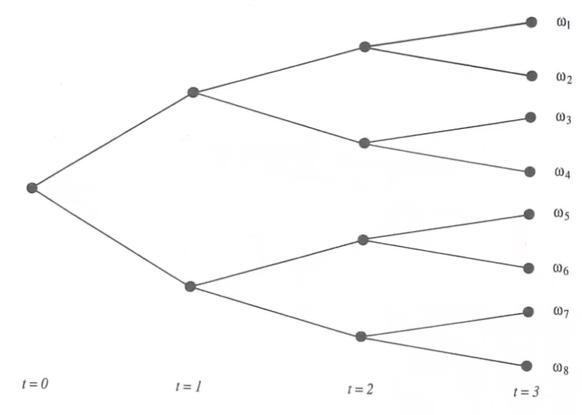
\includegraphics[width=.7\textwidth]{TreeOfInformationStructures.PNG}
    \caption{Tree diagram for the structure of information from \texttt{Example \ref{sec_stochastic_processes_in_discrete_time}.\ref{example_information_structures}.}}
    \label{fig_tree_diagram_of_information_structure}
  \end{figure}

  \begin{figure}[H]
    \centering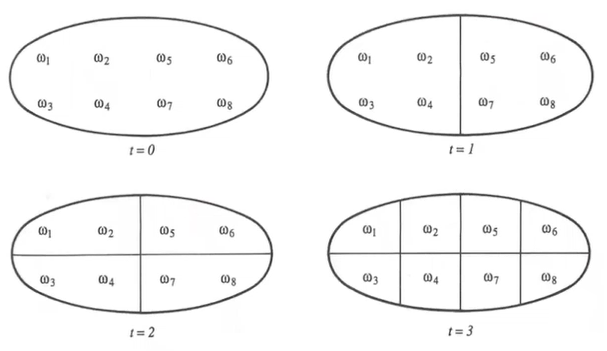
\includegraphics[width=.7\textwidth]{PicturesOfInformationStructures.PNG}
    \caption{A sequence of pictures demonstrating the structure of information \texttt{Example \ref{sec_stochastic_processes_in_discrete_time}.\ref{example_information_structures}.}}
    \label{fig_sequence_of_pictures_of_information_structure}
  \end{figure}

  \begin{example}{}
    Consider an arbitrary sequence $\{\hat{A}_t\}_{t\in[1,T]}$ and some time-point $s<T$. For each $\omega\in \hat{A}_s$ the sequence $\{A_t\}_{t\in[1,T]}$ with $A_T=\{\omega\}$ will coincide with $\{\hat{A}_t\}$ at least until time $t=s$.
    \par The collection of subsets $\{A_{s+1}\}$ that can follow $\hat{A}_s$ forms a partition of $\hat{A}_s$, that is, a collection of disjoint subsets whose union equals $\hat{A}_s$.
    \par In particular, taking $s=0$, we see that the collection $\{A_1\}$ of all possible time-period $t=1$ subsets forms a partition of $\Omega$. This partition is denoted $\mathcal{P}_1$.
    \par Moreover, the collection $\{A_2\}$ of all possible time-period $t=2$ subsets also forms a partition of $\Omega$, denoted $\mathcal{P}_2$.
    Consider \texttt{Example \ref{sec_stochastic_processes_in_discrete_time}.\ref{example_information_structures}} where $K=8$ and $T=3$, the partitions are
    \[\begin{array}{rcl}
      \mathcal{P}_0&=&\big\{\{\omega_1,\omega_2,\omega_3,\omega_4,\omega_5,\omega_6,\omega_7,\omega_8\}\big\}\\
      \mathcal{P}_1&=&\big\{\{\omega_1,\omega_2,\omega_3,\omega_4\},\{\omega_5,\omega_6,\omega_7,\omega_8\}\big\}\\
      \mathcal{P}_2&=&\big\{\{\omega_1,\omega_2\},\{\omega_3,\omega_4\},\{\omega_5,\omega_6\},\{\omega_7,\omega_8\}\big\}\\
      \mathcal{P}_3&=&\big\{\{\omega_1\},\{\omega_2\},\{\omega_3\},\{\omega_4\},\{\omega_5\},\{\omega_6\},\{\omega_7\},\{\omega_8\}\big\}\\
    \end{array}\]
  \end{example}

  \begin{remark}{Visualising Information Structure}
    There are two popular ways to visualise information structure
    \begin{enumerate}
      \item A \textit{Tree Diagram} where each node corresponds to an element $A_t$ of the time $t$ partition and where there is edge arc going from this node to each node corresponding to some $A_{t+1}\subseteq A_t$. (See \texttt{Figure \ref{fig_tree_diagram_of_information_structure}}).
      \item A \textit{Sequence of Pictures} of the same space. (See \texttt{Figure \ref{fig_sequence_of_pictures_of_information_structure}}).
    \end{enumerate}
  \end{remark}

  \begin{definition}{$\sigma$-Algebra $\mathcal{F}_t$}
    A collection $\mathcal{F}$ of subsets of $\Omega$ is called a \textit{$\sigma$-Algebra} on sample space $\Omega$ if
    \begin{enumerate}
      \item $\Omega\in\mathcal{F}$.
      \item $\forall\ F\in\mathcal{F},\ F^c\in\mathcal{F}$.
      \item $\forall\ F,G\in\mathcal{F},\ (F\cup G)\in\mathcal{F}$.
    \end{enumerate}
  \end{definition}

  \begin{proposition}{Generated $\sigma$-Algebra}
    For any partition $\mathcal{P}$ of $\Omega$ we can generate \textit{$\sigma$-Algebra} $\mathcal{F}$ by letting $\mathcal{F}$ be the collection of all unions of elements of $\mathcal{P}$ together with the complements of all such unions.
    \par Hence, the sub-models of the information structure can be organised as a sequence $\{\mathcal{F}_t\}_{t\in[1,T]}$ of \textit{$\sigma$-Algebras}.
  \end{proposition}

  \begin{definition}{Filtration $\mathcal{F}$}
    A \textit{Filtration} is a family of \textit{$\sigma$-Algebras} $\mathcal{F}:=\{\mathcal{F}_t:t=0,1,\dots,T\}$ where
    \begin{enumerate}
      \item $\mathcal{F}_0=\{\emptyset,\Omega\}$.
      \item $\mathcal{F}_T$ consists of all subsets of $\Omega$.
      \item $\mathcal{F}_n\subset\mathcal{F}_{n+1}$ for all $n<T$, by which we mean that each subset of $\mathcal{F}_n$ must be an element of $\mathcal{F}_{n+1}$.
    \end{enumerate}
  \end{definition}

  \begin{example}{$\sigma$-Algebra}
    Consider the context of \texttt{Example \ref{sec_stochastic_processes_in_discrete_time}.\ref{example_information_structures}}. The corresponding filtration is given by
    \[\begin{array}{rcl}
      \mathcal{F}_0&=&\big\{\emptyset,\Omega\big\}\\

      \mathcal{F}_1&=&\big\{\emptyset,\Omega,\{\omega_1,\omega_2,\omega_3,\omega_4\},\{\omega_5,\omega_6,\omega_7,\omega_8\}\big\}\\

      \mathcal{F}_2&=&\big\{\emptyset,\Omega,\{\omega_1,\omega_2\},\{\omega_3,\omega_4\},\{\omega_5,\omega_6\},\{\omega_7,\omega_8\},\{\omega_1,\omega_2,\omega_3,\omega_4\},\\
      &&\ \{\omega_5,\omega_6,\omega_7,\omega_8\},\{\omega_1,\omega_2,\omega_5,\omega_6\},\{\omega_1,\omega_2,\omega_7,\omega_8\},\{\omega_3,\omega_4,\omega_5,\omega_6\},\\
      &&\ \{\omega_3,\omega_4,\omega_7,\omega_8\},\{\omega_1,\omega_2,\omega_3,\omega_4,\omega_5,\omega_6\},\{\omega_1,\omega_2,\omega_3,\omega_4,\omega_7,\omega_8\},\\
      &&\ \{\omega_1,\omega_2,\omega_5,\omega_6,\omega_7,\omega_8\},\{\omega_3,\omega_4,\omega_5,\omega_6,\omega_7,\omega_8\}\big\}\\
    \end{array}\]
    and $\mathcal{F}_3$ contains all the subsets of $\Omega$ (ie $\mathcal{F}_3=2^\Omega$).
  \end{example}

\subsection{Stochastic Processes in Discrete Time}

  \begin{definition}{Stochastic Process $S$}
    A \textit{Stochastic Process} $S$ is a real-valued function $S(t)(\omega)$ of two variables, $t$ and $\omega$.
    \par For each fixed $\omega\in\Omega$ the function mapping $t\to S(t)(\omega)$ is called the \textit{Sample Path}.
    \par For each fixed $t\in[0,T]$ the function mapping $\omega\to S(t)(\omega)$ is a \textit{Random Variable}.
    \par NB - For simplicity, we assume $S(0)$ is constant.
  \end{definition}

  \begin{definition}{Measurable Function}
    A function $\omega\to W(\omega)$ is said to be \textit{Measurable} wrt the \textit{$\sigma$-Algebra} $\mathcal{F}$ if
    \begin{center}
      $\forall\ x\in\reals$ where $W^{-1}(x)\subset\mathcal{F}$ it is true that $W^{-1}(x):=\big\{\omega\in\Omega:W(\omega)=x\big\}$.\footnote{Equivalently, if we know which set of the \textit{$\sigma$-algebra} $\omega$ is in, then we know the value of $W(\omega)$.}
    \end{center}
  \end{definition}

  \begin{example}{Measurable Function}
    Consider random variables $X,Y$ defined as
    \[\begin{array}{rcl}
      X(\omega)&=&\begin{cases}
        5&,\omega\in\{\omega_1,\omega_2,\omega_3,\omega_4\}\\
        7&,\omega\in\{\omega_5,\omega_6,\omega_7,\omega_8\}
      \end{cases}\\
      Y(\omega)&=&\begin{cases}
        8&,\omega\in\{\omega_1,\omega_3,\omega_5,\omega_7\}\\
        6&,\omega\in\{\omega_2,\omega_4,\omega_6,\omega_8\}
      \end{cases}
    \end{array}\]
    Then, by the notation of \texttt{Example \ref{sec_stochastic_processes_in_discrete_time}.\ref{example_information_structures}}, we have that
    \begin{itemize}
      \item $X$ is \textit{Measurable} wrt $\mathcal{F}_1,\mathcal{F}_2,\mathcal{F}_3$ as $\big\{\{\omega_1,\omega_2,\omega_3,\omega_4\},\{\omega_5,\omega_6,\omega_7,\omega_8\},\emptyset\big\}\subset\mathcal{F}_1$.
      \item $Y$ is \underline{not} \textit{Measurable} wrt $\mathcal{F}_1,\mathcal{F}_2$, but is measurable wrt $\mathcal{F}_3$, as $\{\omega_1,\omega_3,\omega_5,\omega_7\}\not\in\mathcal{F}_1$.
    \end{itemize}
  \end{example}

  \begin{remark}{Measurable}
    If a function $X$ is \textit{Measurable} wrt $\mathcal{F}_t$ then it will be \textit{Measurable} wrt $\mathcal{F}_{t+1}$, as $\mathcal{F}_t\subseteq\mathcal{F}_{t+1}$.
  \end{remark}

  \begin{definition}{Adapted}
    A \textit{Stochastic Process} $S=\{S(t):t=0,1,\dots,T\}$ is said to be \textit{Adapted} to the \textit{Filtration} $\mathcal{F}=\{\mathcal{F}_t:t=0,1,\dots,T\}$ if for every $t=0,\dots,T$ the random variable $S(t)$ is \textit{Measurable} wrt $\mathcal{F}_t$.
  \end{definition}

  \begin{remark}{Adapted Filtrations in Practice}
    In practice we often define the \textit{Stochastic Process} $S$ first and use the so-called ``\textit{Natural Filtration}'', defined as
    \begin{enumerate}
      \item For each $t=0,1,\dots,T$ let $\mathcal{P}_t$ be the partition of $\Omega$ st the \textit{Stochastic Process} $\{S(0),\dots,S(t)\}$ takes the same value for each $\omega\in A$, for each subset $A\in\mathcal{P}_t$.
      \item Let $\mathcal{F}_t$ be the \textit{$\sigma$-Algebra} generated by $\mathcal{P}_t$.
      \item Then $\mathcal{F}:=\{\mathcal{F}_t:t=0,1,\dots,T\}$ is called the filtration \textit{Generated} by the \textit{Stochastic Process} $S$.
    \end{enumerate}
  \end{remark}

  \begin{example}{}\label{example_2_13}
    Consider the setting it \texttt{Example \ref{sec_stochastic_processes_in_discrete_time}.\ref{example_information_structures}} and let $S(t)$ be the upwards movements in the value of the asset by time $t$. Then $S(t)$ generates the \textit{Filtration} above.
    \par This can be summarised in the table
    \begin{center}
      \begin{tabular}{c|cccc}
        $\omega_k$&$t=0$&$t=1$&$t=2$&$t=3$\\\hline
        $\omega_1$&$S(t)=0$&$S(t)=1$&$S(t)=2$&$S(t)=3$\\
        $\omega_2$&$S(t)=0$&$S(t)=1$&$S(t)=2$&$S(t)=2$\\
        $\omega_3$&$S(t)=0$&$S(t)=1$&$S(t)=1$&$S(t)=2$\\
        $\omega_4$&$S(t)=0$&$S(t)=1$&$S(t)=1$&$S(t)=1$\\
        $\omega_5$&$S(t)=0$&$S(t)=0$&$S(t)=1$&$S(t)=2$\\
        $\omega_6$&$S(t)=0$&$S(t)=0$&$S(t)=1$&$S(t)=1$\\
        $\omega_7$&$S(t)=0$&$S(t)=0$&$S(t)=0$&$S(t)=1$\\
        $\omega_8$&$S(t)=0$&$S(t)=0$&$S(t)=0$&$S(t)=0$
      \end{tabular}
    \end{center}
  \end{example}

  \begin{definition}{Random Walk}
    Let $X_t:=X_0+Y_1+\dots+Y_t$ where $Y_1,\dots,Y_t$ are iid random variables with finite variance $\sigma^2$ and mean $mean$. Then $\{X_t:t\geq0\}$ is a \textit{Random Walk}.
    \par We say that $\{X_t:t\geq0\}$ is a \textit{Simple Random Walk} if $Y_i$ takes only the values 1 with probability $p$ and -1 with probability $1-p$.
  \end{definition}

  \begin{proposition}{Distribution of Simple Random Walk Values}
    A \textit{Simple Random Walk} takes values $y$ at time-point $t$ iff exactly $\frac{t+y}2$ of $Y_1,\dots,Y_t$ are equal to 1, and the remaining $\frac{t-y}2$ equal -1.
    \[ \forall\ t\geq0,y\in\{-t,-t+2,\dots,t-2,t\},\quad\prob(X_t=y)={t\choose {\frac{t+y}2}}p^{(t+y)/2}(1-p)^{(t-y)/2} \]
  \end{proposition}

\subsection{Conditional Expectations}

  \begin{definition}{Conditional Expectation $\expect[\cdot|\cdot]$}
    For a finite \textit{Sample Space} $\Omega$ the \textit{Conditional Expectation} of a discrete RV $Y$ given the event $A$ $\expect[Y|A]$ is defined as
    \[ \expect[Y|A]=\sum_yy\prob(Y=y|A) \]
    This \textit{Conditional Expectation} maps from the events $A$ to the real numbers.
  \end{definition}

  \begin{remark}{Rewriting Conditional Expectation}
    We can rewrite the \textit{Conditional Expectation} as
    \[\begin{array}{rcl}
      \expect[Y|A]&=&\sum_yy\frac{\prob(Y(\omega)=y,A)}{\prob(A)}\\
      &=&\sum_{\omega\in A}Y(\omega)\frac{\prob(\omega)}{\prob(A)}
    \end{array}\]
  \end{remark}

  \begin{example}{Conditional Expectation}
    Consider \texttt{Example \ref{sec_stochastic_processes_in_discrete_time}.\ref{example_2_13}} with $\omega_i$ having probability 1/8.
    \begin{itemize}
      \item If $A:=\{\omega_1,\omega_2,\omega_3,\omega_4\}$ then
      \[ \expect[S_3|A]=\frac{(3+2+2+1)(1/8)}{1/2}=2 \]
      \item If $A:=\{\omega_5,\omega_6,\omega_7,\omega_8\}$ then
      \[ \expect[S_3|A]=\frac{(2+1+1+0)(1/8)}{1/2}=1 \]
    \end{itemize}
  \end{example}

  \begin{definition}{Conditional Expectation /w $\sigma$-Algebra}
    Let $\mathcal{F}$ be a \textit{$\sigma$-algebra} and $\mathcal{P}$ be the corresponding \textit{Partition} of $\Omega$.
    \par We define the \textit{Conditional Expectation} of RV $Y$ give \textit{$\sigma$-algebra} $\mathcal{F}$ as
    \[ \expect[Y|\mathcal{F}]=\sum_{A\in\mathcal{P}}\expect[Y|A]\indexed_A \]
    This is a random-variable\footnote{Not a sum, as there is one $A$ st $\indexed_A=1$ (the rest equal zero)} which is \textit{Measurable} wrt $\mathcal{F}$. And,
    \[ \forall\ \omega\in A,\ \expect[Y|\mathcal{F}](\omega)=\expect[Y|A] \]
  \end{definition}

  \begin{example}{Conditional Expectation /w $\sigma$-Algebras}
    Consider \texttt{Example \ref{sec_stochastic_processes_in_discrete_time}.\ref{example_2_13}} with $\omega_i$ having probability 1/8.
    \par Recall that $\mathcal{F}_1=\big\{\emptyset,\Omega,\{\omega_1,\omega_2,\omega_3,\omega_4\},\{\omega_5,\omega_6,\omega_7,\omega_8\}\big\}$.
    Then
    \[ \expect[S_3|A]=\begin{cases}2&\text{if }A=\{\omega_1,\omega_2,\omega_3,\omega_4\}\\1&\text{if }A=\{\omega_5,\omega_6,\omega_7,\omega_8\}\end{cases} \]
    Hence $\expect[S_3|\mathcal{F}_1]$ is a random variable with
    \[ \expect[S_3|\mathcal{F}](\omega_i)=\begin{cases}2&\text{if }i=1,2,3,4\\1&\text{if }i=5,6,7,8\end{cases} \]
    This random variable is \textit{$\mathcal{F}_1$-Measurable}.
    \par Observer that
    \[\begin{array}{rcl}
      \expect[\expect[S_3|\mathcal{F}_1]]&=&\sum_i\prob(\omega_i)\expect[S_3|\mathcal{F}_1](\omega_i)\\
      &=&2\cdot\frac48+1\cdot\frac48=\frac32=\expect[S_3]\footnotemark
    \end{array}\]
    \footnotetext{This is the ``Tower Law''}
    Note that if
    \[ Y(\omega_i)=\begin{cases}7&\text{if }i\leq4\\1&\text{if }i\geq5\end{cases}\implies\expect[Y|\mathcal{F}_1]=Y \]
    Moreover, If $Z=\indexed\{\text{3rd move is up}\}$ then $|$ is independent of $\mathcal{F}_1$ and
    \[ \expect[Z|\mathcal{F}_1]=\frac12=\expect[Z] \]
  \end{example}

  \begin{theorem}{Properties of Conditional Expectation}\label{the_properties_of_conditional_expectation}
    Let $Y$ be a random variable and $\mathcal{F},\mathcal{F}_1,\mathcal{F}_2$ be \textit{$\sigma$-algebras} with $\mathcal{F}_1\subset\mathcal{F}_2$.
    \par\textit{Conditional Expectations} satisfy the following properties:
    \begin{enumerate}
      \item $\expect[\expect[Y|\mathcal{F}]]=\expect[Y]$. (The ``Tower Law'')
      \item $\expect[\expect[Y|\mathcal{F}_2]|\mathcal{F}_1]=\expect[Y|\mathcal{F}_1]=\expect[\expect[Y|\mathcal{F}_1]\mathcal{F}_2]$. (The ``Generalised Tower Law'')
      \item If $X$ is a random variable which is \textit{Measurable} wrt $\mathcal{F}$ then $\expect[XY|\mathcal{F}]=X\expect[Y|\mathcal{F}]$ and $\expect[X|\mathcal{F}]=X$.\footnote{As $X$ is measurable wrt $\mathcal{F}$ all information is known about it, and thus can treat it as a scalar.}
      \item If $Y$ is independent of $\mathcal{F}$\footnote{$\forall\ A\in\mathcal{P}$ the distribution of $Y$ is independent of $A$} then $\expect[Y|\mathcal{F}]=\expect[Y]$.
    \end{enumerate}
  \end{theorem}

  \begin{proof}{\texttt{Theorem \ref{sec_stochastic_processes_in_discrete_time}.\ref{the_properties_of_conditional_expectation} i)}}
    \everymath={\displaystyle}
    \[\begin{array}{rcl}
      \expect[\expect[Y|\mathcal{F}]]&=&\expect\left[\sum_{A\in\mathcal{P}}\expect[Y|A]\indexed_A\right]\text{ by def. cond. expectation}\\
      &=&\sum_{A\in\mathcal{P}}\expect[\indexed_A]\expect[Y|A]\\
      &=&\sum_{A\in\mathcal{P}}\left(\sum_{\omega\in\Omega}\indexed_A(\omega)\prob(\omega )\right)\cdot\left(\sum_{\omega\in A}\frac{Y(\omega)\prob(\omega)}{\prob(A)}\right)\\
      &=&\sum_{A\in\mathcal{P}}\prob(A)\left(\sum_{\omega\in A}\frac{Y(\omega)\prob(\omega)}{\prob(A)}\right)\\
      &=&\sum_{A\in\mathcal{P}}\sum_{\omega\in A}Y(\omega)\prob(\omega)\\
      &=&\expect[Y]
    \end{array}\]
    \proved
  \end{proof}

  \begin{proof}{\texttt{Theorem \ref{sec_stochastic_processes_in_discrete_time}.\ref{the_properties_of_conditional_expectation} ii)}}
    \everymath={\displaystyle}
    \[\begin{array}{rcl}
      \expect[\expect[Y|\mathcal{F}_2]\mathcal{F}_1]&=&\expect\left(\sum_{B\in\mathcal{P}_2}\expect[Y|B]\indexed_B\big|\mathcal{F}_1\right)\\
      &=&\sum_{B\in\mathcal{P}_2}\expect[Y|B]\expect[\indexed_B|\mathcal{F}_1]\\
      &=&\sum_{B\in\mathcal{P}_2}\expect[Y|B]\sum_{A\in\mathcal{P}_1}\expect[1_B|A]\indexed_A\\
      &=&\sum_{A\in\mathcal{P}_1}\sum_{B\in\mathcal{P}_2}\expect[Y|B]\expect[1_B|A]\indexed_A\\
      &=&\sum_{A\in\mathcal{P}_1}\sum_{B\in\mathcal{P}_2}\expect[Y|B]\frac{\prob(A\cap B)}{\prob(A)}\indexed_A\\
    \end{array}\]
    Since the partition $\mathcal{P}_2$ is finer than $\mathcal{P}_1$  for all $B\in\mathcal{P}_2$ and $A\in\mathcal{P}_1$, either $B\subset A$ or $B\cap A=\emptyset$.
    \par Thus
    \[\begin{array}{rcl}
      \expect[\expect[Y|\mathcal{F}_2]|\mathcal{F}_1]&=&\sum_{A\in\mathcal{P}_1}\sum_{B\in\mathcal{P}_2,B\subset A}\expect[Y|B]\frac{\prob(B)}{\prob(A)}\indexed_A\\
      &=&\sum_{A\in\mathcal{P}_1}\sum_{B\in\mathcal{P}_2,B\subset A}\left(\sum_{\omega\in B}Y(\omega)\frac{\prob(\omega)}{\prob(B)}\right)\frac{\prob(B)}{\prob(A)}\indexed_A\\
      &=&\sum_{A\in\mathcal{P}_1}\sum_{\omega\in A}Y(\omega)\frac{\prob(\omega)}{\prob(A)}\indexed_A\\
      &=&\sum_{A\in\mathcal{P}_1}\expect[Y|A]\indexed_A\\
      &=&\expect[Y|\mathcal{F}_1]
    \end{array}\]
    \proved
  \end{proof}

  \begin{proof}{\texttt{Theorem \ref{sec_stochastic_processes_in_discrete_time}.\ref{the_properties_of_conditional_expectation} iii)}}\label{proof_conditional_expectation_property_iii}
    \everymath={\displaystyle}
    Since $S$ is \textit{Measurable} it is constant on sets of $\mathcal{P}$ so we can write
    \[ X=\sum_{A\in\mathcal{P}} x_A\indexed_A \]
    with suitable scalars $x_A\in\reals$. Then
    \[\begin{array}{rcl}
      \expect[XY|\mathcal{F}]&=&\sum_{A\in\mathcal{P}}\expect[XY|A]\indexed_A\\
      &=&\sum_{A\in\mathcal{P}}\expect[x_AY|A]\indexed_A\\
      &=&\sum_{A\in\mathcal{P}}x_A\expect[Y|A]\indexed_A\\
      &=&\sum_{A\in\mathcal{P}}X\expect[Y|A]\indexed_A\footnotemark\\
      &=&X\sum_{A\in\mathcal{P}}\expect[Y|A]\indexed_A\\
      &=&X\expect[Y|\mathcal{F}]
    \end{array}\]
    \footnotetext{This holds as $\indexed_A=1$ for only one specific $A$.}
    Consider the special case where $Y=1$, then it follows that $\expect[X|\mathcal{F}]=X$.\proved
  \end{proof}

  \begin{proof}{\texttt{Theorem \ref{sec_stochastic_processes_in_discrete_time}.\ref{the_properties_of_conditional_expectation} iv)}}
    \everymath={\displaystyle}
    If $Y$ is independent of $\mathcal{F}$ then for all $A\in\mathcal{F}$
    \[\begin{array}{rcl}
      \expect[Y|A]&=&\sum_yy\prob(Y=y|A)\\
      &=&\sum_yy\prob(Y=y)\\
      &=&\expect[Y]
    \end{array}\]
    \proved
  \end{proof}

  \begin{proposition}{Conditional Expectation for Non-Finite Sample Spaces}\label{prop_conditional_expectation_for_non_finite_sample_space}
    Let $Y$ be a RV, then the \textit{Conditional Expectation} $\expect[Y|\mathcal{F}]$ is the unique random variable st
    \begin{enumerate}
      \item $\expect[Y|\mathcal{F}]$ is $\mathcal{F}$-Measurable.
      \item $\forall\ A\in\mathcal{F},\ \expect[\expect[Y|\mathcal{F}]\cdot\indexed_A]=\expect[Y\indexed_A]$.
    \end{enumerate}
  \end{proposition}

  \begin{proof}{\texttt{Proposition \ref{sec_stochastic_processes_in_discrete_time}.\ref{prop_conditional_expectation_for_non_finite_sample_space}}}
    For an arbitrary event $A\in\mathcal{F}$ the indicator function $\indexed_A$ is \textit{$\mathcal{F}$-Measurable} and thus $\expect[\indexed_AY|\mathcal{F}]=\indexed_A\expect[Y|\mathcal{F}]$ by \texttt{Theorem \ref{sec_stochastic_processes_in_discrete_time}.\ref{the_properties_of_conditional_expectation}}.
    \par Hence, for all $A\in\mathcal{F}$
    \[ \expect[\expect[Y|\mathcal{F}]\cdot\indexed_A]=\expect[\expect[\indexed_AY|\mathcal{F}]]=\expect[\indexed_AY] \]
    On the other hand, suppose $X$ is \textit{$\mathcal{F}$-Measurable} and satisfies
    \[ \expect[X\indexed_A]=\expect[Y1_A]\ \forall\ A\in\mathcal{F} \]
    Then write $X$ as in \texttt{Proof \ref{sec_stochastic_processes_in_discrete_time}.\ref{proof_conditional_expectation_property_iii}} $X=\sum_{A\in\mathcal{P}}x_A\indexed_A$.
    \par It follows that $\forall\ A\in\mathcal{P},\ \expect[X\indexed_A]=x_A\prob(A)$ and thus
    \[\begin{array}{rcl}
      \expect[Y\indexed_A]&=&\sum_{\omega\in A}Y(\omega)\prob(\omega)\\
      &=&\frac{\prob(A)}{\prob(A)}\sum_{\omega\in A}Y(\omega)\prob(\omega)\\
      &=&\prob(A)\sum_{\omega\in A}\frac{Y(\omega)\prob(\omega)}{\prob(A)}\\
      &=&\prob(A)\expect[Y|A]
    \end{array}\]
    Thus
    \[ x\prob(A)=\expect[X\indexed_A]=\expect[Y\indexed_A]=\prob(A)\expect[Y|A] \]
    Therefore, we have found that $x_A=\expect[Y|A]\ \forall\ A\in\mathcal{P}$ where $\mathcal{P}$ is the partition which corresponds to \textit{$\sigma$-algebra} $\mathcal{F}$.
    \par Moreover, $X=\expect[Y|\mathcal{F}]$.
  \end{proof}

\subsection{Martingales}

  \begin{definition}{Martingale $Z$}\label{def_martingales}
    Let $Z:=\{Z_t:t=0,1,\dots,T\}$ be an \textit{Adapted Stochastic Process} defined on a \textit{Sample Space} $\Omega$ with a filtration $\{\mathcal{F}_t\}$.
    \par The process $Z$ is said to be a \textit{Martingale} if
    \[ \expect[Z_t|\mathcal{F}_{t-1}]=Z_{t-1}\ \forall\ t\geq1 \]
  \end{definition}

  \begin{definition}{Super-Martingale $Z$}
    Let $Z:=\{Z_t:t=0,1,\dots,T\}$ be an \textit{Adapted Stochastic Process} defined on a \textit{Sample Space} $\Omega$ with a filtration $\{\mathcal{F}_t\}$.
    \par The process $Z$ is said to be a \textit{Super-Martingale} if
    \[ \expect[Z_t|\mathcal{F}_{t-1}]\leq Z_{t-1}\ \forall\ t\geq1 \]
  \end{definition}

  \begin{definition}{Sub-Martingale $Z$}
    Let $Z:=\{Z_t:t=0,1,\dots,T\}$ be an \textit{Adapted Stochastic Process} defined on a \textit{Sample Space} $\Omega$ with a filtration $\{\mathcal{F}_t\}$.
    \par The process $Z$ is said to be a \textit{Sub-Martingale} if
    \[ \expect[Z_t|\mathcal{F}_{t-1}]\geq Z_{t-1}\ \forall\ t\geq1 \]
  \end{definition}

  \begin{remark}{Super- vs Sub-Martingale}
    You should think of a \textit{Super-Martingale} as a process where the current value provides an \underline{upper}-bound on the next value, and a \textit{Sub-Martingale} as a process where the current value provides a \underline{lower}-bound on the next value.
  \end{remark}

  \begin{theorem}{When is an Adapted Stochastic Process a Martingale?}\label{the_adapted_stochastic_process_and_martingales}
    An \textit{Adapted Stochastic Process $Z$} is a \textit{Martingale} iff
    \[ \expect[Z_t|\mathcal{F}_s]=Z_s\ \forall\ t\geq s \]
    Corresponding results (with equality swapped out) hold for super- and sub-martingales.
  \end{theorem}

  \begin{proof}{\texttt{Theorem \ref{sec_stochastic_processes_in_discrete_time}.\ref{the_adapted_stochastic_process_and_martingales}}}
    \begin{itemize}
      \item[$\Longleftarrow$]Clearly, if the equation in \texttt{Theorem \ref{sec_stochastic_processes_in_discrete_time}.\ref{the_adapted_stochastic_process_and_martingales}} holds then \texttt{Definition \ref{sec_stochastic_processes_in_discrete_time}.\ref{def_martingales}} holds.
      \item[$\Longrightarrow$] Assume $Z$ is a \textit{Martingale}. Then \texttt{Theorem \ref{sec_stochastic_processes_in_discrete_time}.\ref{the_properties_of_conditional_expectation}} implies that
      \[\begin{array}{rcl}
        \expect[Z_t|\mathcal{F}_s]&=&\expect\big[\expect[Z_t|\mathcal{F}_{t-1}]|\mathcal{F}_s\big]\\
        &=&\expect[Z_{t-1}|\mathcal{F}_s]\text{ as }Z\text{ is a martingale}\\
        &=&\expect[Z_s|\mathcal{F}_s]\text{ by repetition}\\
        &=&\expect[Z_s]=Z_s
      \end{array}\]
    \end{itemize}
    A similar proof is done for super- and sub-martingales.
  \end{proof}

  \begin{example}{Martingales}\label{example_martingales}
    Let $\{X_t\}_{t\geq0}$ be a simple random walk with parameter $p$ and $\mathcal{F}_t$ be the \textit{$\sigma$-algebra} generated by $(X_t)$. Then
    \begin{enumerate}
      \item $\{X_t\}_{t\geq0}$ is a \textit{Martingale} if $p=1/2$ as there is an equal probability of stepping up and stepping down.
      \item $\{X_t\}_{t\geq0}$ is a \textit{Super-Martingale} if $p\leq1/2$ as there is a greater probability of stepping down than stepping up.
      \item $\{X_t\}_{t\geq0}$ is a \textit{Sub-Martingale} if $p\geq1/2$ as there is a greater probability of stepping up than stepping down.
      \item If $p=1/2$ then the process $\{Z_t\}_{t\geq0}$ defined st $Z_t:=X_t^2-t$ for $t=0,1,\dots$ is a \textit{Martingale}
      \item If $p\neq1/2$ then the processes $\{L_t\}_{t\geq0}$ \& $\{M_t\}_{t\geq0}$ defined by $L_0=1,\ L_t=\left(\frac{1-p}p\right)^{X_t}$ and $M_t=X_t-t(2p-1)$ are both \textit{Martingales}\footnote{Proved in a homework}.
    \end{enumerate}
  \end{example}

  \begin{proof}{\texttt{Example \ref{sec_stochastic_processes_in_discrete_time}.\ref{example_martingales}} i)-iii) }
    Since $\mathcal{F}_t$ is the natural filtration, then $\{X_t\}$ is $\mathcal{F}_t$-measurable and $Y_t$ is independent of $\mathcal{F}_{t-1}$. Therefore by \texttt{Theorem \ref{sec_stochastic_processes_in_discrete_time}.\ref{the_properties_of_conditional_expectation}} we have that
    \[\begin{array}{rcl}
      \expect[X_t|\mathcal{F}_{t-1}]&=&\expect[X_{t-1}+Y_t|\mathcal{F}_{t-1}]\\
      &=&\expect[X_{t-1}|\mathcal{F}_{t-1}]+\expect[Y_t|\mathcal{F}_{t-1}]\\
      &=&X_{t-1}+\expect[Y_t]
    \end{array}\]
    \begin{itemize}
      \item If $p=1/2$ then $\expect[Y_t]=0\implies\expect[X_t|\mathcal{F}_{t-1}]=X_{t-1}$, the definition of a \textit{Martingale}.
      \item If $p\leq1/2$ then $\expect[Y_t]\leq0\implies\expect[X_t|\mathcal{F}_{t-1}]\leq X_{t-1}$, the definition of a \textit{Super-Martingale}.
      \item If $p\geq1/2$ then $\expect[Y_t]\geq0\implies\expect[X_t|\mathcal{F}_{t-1}]\geq X_{t-1}$, the definition of a \textit{Sub-Martingale}.
    \end{itemize}
  \end{proof}

  \begin{proof}{\texttt{Example \ref{sec_stochastic_processes_in_discrete_time}.\ref{example_martingales}} iv) }
    Note that
    \[\begin{array}{rcl}
      \expect[Z_t|\mathcal{F}_{t-1}]&=&\expect[X_t^2-t|\mathcal{F}_{t-1}]\\
      &=&\expect[(X_{t-1}+Y_t)^2|\mathcal{F}_{t-1}]-t\\
      &=&\expect[X_{t-1}^2|\mathcal{F}_{t-1}]+2\expect[X_tY_t|\mathcal{F}_{t-1}]+\expect[Y_t^2|\mathcal{F}_{t-1}]t\\
      &=&X_{t-1}^2+2X_{t-1}\underbrace{\expect[Y_t|\mathcal{F}_{t-1}]}_{=\expect[Y_t]=0}+\underbrace{\expect[Y_t^2]}_{=1\footnotemark}-t\\
      &=&X_{t-1}^2+0+1-t\\
      &=&X_{t-1}^2-(t-1)=Z_{t-1}
    \end{array}\]
    This shows that the $Z_t$ we defined fulfils the definition of a \textit{Martingale}.
    \footnotetext{$Y_t$ only takes values $\{-1,1\}$ so $Y_t^2=1$ always.}
  \end{proof}

\subsection{Stopping Times $\tau$}

    \begin{remark}{Stopping Times \& Finance}
      \textit{Stopping Times} are useful for analysing American options.
    \end{remark}

    \begin{definition}{Stopping Time $\tau$}
      Let $\Omega$ be a \textit{Sample Space} with a filtration $\{\mathcal{F}_t\}_{t\in\nats_0}$.
      \par A \textit{Stopping Time} is a random variable $\tau$ which takes values in the set $\{0,1,\dots,\infty\}$\footnote{$\infty$ is used for events which never occur.} st each event of the form $\{\tau\leq t\}$ from some $t$ is an element of the \textit{$\sigma$-algebra} $\mathcal{F}_t$.\footnote{Thus, we can determine whether $\{\tau\leq t\}$ has occurred just by observing $\mathcal{F}_t$ (ie all the information available at time-point $t$).}
      \par A \textit{Stopping Time} is said to be \textit{Bounded} if $\exists\ k$ st $\prob(\tau<t)=1$.
    \end{definition}

    \begin{example}{Stopping Time}
      Consider the following events
      \begin{itemize}
        \item ``RBS shares hit 100p.'' - This is a \textit{Stopping Time} event.
        \item ``RBS shares hit their maximum.'' - This is \underline{not} a \textit{Stopping Time} event.
      \end{itemize}
    \end{example}

    \begin{theorem}{Stopping Times \& $\sigma$-Algebras}\label{the_stopping_times_and_sigma_algebras}
      A random variable $\tau$ is a \textit{Stopping Time} \underline{iff} each event of the form $\{\tau=t\}$ for some $t$ is an element of the \textit{$\sigma$-Algebra} $\mathcal{F}_t$.
    \end{theorem}

    \begin{proof}{\texttt{Theorem \ref{sec_stochastic_processes_in_discrete_time}.\ref{the_stopping_times_and_sigma_algebras}} }
      \everymath={\displaystyle}
      \begin{itemize}
        \item[$\Longleftarrow$] $ \{\tau=t\}=\big(\underbrace{\{\tau\leq t\}}_{\in\mathcal{F}_t}\setminus\underbrace{\{\tau\leq t-1\}}_{\in\mathcal{F}_t}\big)\in\mathcal{F}_t$
        \item[$\Longrightarrow$] $\{\tau\leq t\}=\bigcup\limits_{k\leq t}\underbrace{\{\tau=k\}}_{\in\mathcal{F}_t}\in\mathcal{F}_t$
      \end{itemize}
      Thus the result holds in both directions.
    \end{proof}

    \begin{theorem}{Stopping Time for an Adapted Stochastic Process}\label{the_stopping_time_for_an_adapted_stochastic_process}
      Let $\{X_t\}_{t\in\nats_0}$ be an \textit{Adapted Stochastic Process} and $c\in\reals$.
      \par A \textit{Stopping Time} $\tau_c$ can be defined as $\tau_c=\inf\{t\geq0:X_t\geq \}$\footnote{The event which stops the moment $X_t$ reaches $c$}.
    \end{theorem}

    \begin{proof}{\texttt{Theorem \ref{sec_stochastic_processes_in_discrete_time}.\ref{the_stopping_time_for_an_adapted_stochastic_process}}}
      We note that $\tau_c\leq t$ \underline{iff} $\exists\ k\leq t$ st $X_k\geq c$.
      \par Therefore
      \[ \{\tau_c\leq t\}=\bigcup\limits_{k\leq t}\underbrace{\{X_k\geq c\}}_{\in\mathcal{F}_t}\in\mathcal{F}_t \]
      Thus $\tau_c$ is a \textit{Stopping Time}.
    \end{proof}

    \begin{theorem}{Optional Sampling Theorem\footnote{AKA \textit{Optional Stopping Theorem}} - Martingales}\label{the_optional_sampling_theorem}
      Let $\tau$ be a \textit{Bounded Stopping Time} and $X=\{X_t\}_{t\in\nats_0}$ be a \textit{Martingale}. Then
      \[ \expect[X_\tau]=\expect[X_0]=X_0 \]
    \end{theorem}

    \begin{theorem}{Optional Sampling Theorem - Super-Martingales}\label{the_optional_sampling_theorem_supermartingales}
      Let $\tau$ be a \textit{Bounded Stopping Time} and $X=\{X_t\}_{t\in\nats_0}$ be a \textit{Super-Martingale}. Then
      \[ \expect[X_\tau]=\leq \expect[X_0] \]
    \end{theorem}

    \begin{proof}{\texttt{Theorem \ref{sec_stochastic_processes_in_discrete_time}.\ref{the_optional_sampling_theorem}}}
      \everymath={\displaystyle}
      Assume that $\tau\leq K$ and write
      \[ X_{\tau(\omega)}(\omega)=\sum_{t=0}^KX_t(\omega)\indexed\{\tau(\omega)=t\}\footnotemark \]
      \footnotetext{This is not really a sum, due to the indicator function $\indexed$ meaning only one value is non-zero.}
      Then
      \[\begin{array}{rcl}
        \expect[X_\tau]&=&\expect\left[\sum_{t=0}^KX_t\indexed\{\tau=t\}\right]\\
        &=&\sum_{t=0}^K\expect[X_t\indexed\{\tau=t\}]\\
        &=&\sum_{t=0}^K\expect[\expect[X_K|\mathcal{F}_t]\indexed\{\tau=t\}]
      \end{array}\]
      Using that since $\tau$ is a \textit{Stopping Time}, then the event $\{\tau=t\}$ is measurable wrt $\mathcal{F}_t$. Thus $\expect[X_K|\mathcal{F}_t]\indexed\{\tau=t\}=\expect[X_K\indexed\{\tau=t\}|\mathcal{F}_t]$.
      \[\begin{array}{rcl}
        &=&\sum_{t=0}^K\expect[\expect[X_K\indexed\{\tau=t\}|\mathcal{F}_t]]\\
        &=&\sum_{t=0}^K\expect[X_K\indexed\{\tau=t\}]\text{ by Tower Law}\\
        &=&\expect\left[X_K\sum_{t=0}^K\indexed\{\tau=t\}\right]\\
        &=&\expect[X_K\cdot1]=\expect[X_K]\\
        &=&\expect[X_0]=X_0
      \end{array}\]
    \end{proof}

    \begin{example}{Gambler's Ruin}\label{example_gamblers_ruin}
      Consider a gambler with an initial wealth of £$C$. He gambles by guessing whether a coin flip results in heads or tails. If he guess correctly then he receives £1 and he is wrong he loses £1. The game ends when he either becomes bankrupt or he reaches a wealth of £$C+G$ where $G>0$.
    \end{example}

    \begin{proposition}{Gambler's Ruin}\label{prop_gamblers_ruin}
      \everymath={\displaystyle}
      Let $\{X_t\}_{t\geq0}$ be a \textit{Simple Random Walk} with parameter $p$ and $X_0=0$, and $C,G>0$. Define the \textit{Stopping-Time} event $\tau=\inf\{t:X_t=G\text{ or }X_t=-C\}$\footnote{The event the game in \texttt{Example \ref{sec_stochastic_processes_in_discrete_time}.\ref{example_gamblers_ruin}}}.
      \par If $p=1/2$ then
      \[\begin{array}{rcl}
        \prob(X_\tau=G)&=&\frac{C}{C+G}\\
        \prob(X_\tau=-C)&=&\frac{G}{C+G}\\
        \expect[\tau]&=&CG
      \end{array}\]
      \par Else, if $p\neq1/2$ then
      \[\begin{array}{rcl}
        \prob(X_\tau=G)&=&\frac{1-\left(\frac{p}{1-p}\right)^C}{\left(\frac{p}{1-p}\right)^G-\left(\frac{p}{1-p}\right)^C}\\
        \prob(X_\tau=-C)&=&1-\prob(X_\tau=G)\\
        \expect[\tau]&=&\frac{G\prob(X_\tau=G)+(-C)\prob(X_\tau)=-C}{2p-1}
      \end{array}\]
    \end{proposition}

    \begin{proof}{\texttt{Proposition \ref{sec_stochastic_processes_in_discrete_time}.\ref{prop_gamblers_ruin}}}
      \everymath={\displaystyle}
      We want to apply the \textit{Optitional Stopping Theorem} (\texttt{Theorem \ref{sec_stochastic_processes_in_discrete_time}.\ref{the_optional_sampling_theorem}}).
      \par The \textit{Stopping Time} $\tau$ is not bounded, but $X_\tau$ is bounded. Therefore we can use one of the alternative versions of the \textit{Optional Stopping Theorem} provided that $\prob(\tau<\infty=1)$.
      \par Note that whenever there is a run of at least $k=C+G$ successive 1's in the process $Y$ which defines $X$, the process will stop and $\tau<\infty$. Thus for all $m$
      \[\begin{array}{rcl}
        \prob(\tau>km)&=&\prob(\text{No run of k 1's in }Y_1\text{ to }Y_{mk})\\
        &=&\prod_{j=0}^{n-1}\prob(\text{No run of k 1's in }Y_{jk+1}\text{ to }Y_{(j+1)k})\\
        &=&(1-p^k)^m\\
        \implies\prob(\tau<\infty)&=&1
      \end{array}\]
      \begin{enumerate}
        \item Consider the case $p=1/2$. Using the \textit{Optional Stopping Theorem} we can deduce that
        \[\begin{array}{rrcl}
          &0&=&\expect[X_\tau]\\
          &&=&G\prob(X_\tau=G)+(-C)\prob(X_\tau=-C)\\
          &&=&G\prob(X_\tau=G)+(-C)(1-\prob(X_\tau=G))\\
          \implies&C&=&(G+C)\prob(X_\tau=G)\\
          \implies&\prob(X_\tau=G)&=&\frac{C}{(G+C)}\\
          \text{and}&\prob(X_\tau=-C)&=&1-\frac{C}{(G+C)}=\frac{G}{G+C}\\
        \end{array}\]
        We determine $\expect[X_\tau]$ by applying the \textit{Optional Stopping Theorem} to the process $\{Z_t\}_{t\geq0}$ where $Z_t:=X_t^2-t$. We know $\{Z_t\}_{t\geq0}$ is a \textit{Martingale} from \texttt{Example \ref{sec_stochastic_processes_in_discrete_time}.\ref{example_martingales} iv)}.
        \par As $\{Z_t\}_{t\geq0}$ is a \textit{Martingale} it holds that
        \[ 0=\expect[Z_0]=\expect[Z_\tau]=\expect[X_\tau^2-\tau] \]
        Thus, we obtain that
        \[\begin{array}{rcl}
          \expect[\tau]&=&\expect[X_\tau^2]\\
          &=&G^2\prob(X_\tau=G)+C^2\prob(X_\tau=-C)\\
          &=&G^2\frac{C}{C+G}+C^2\frac{G}{C+G}\\
          &=&CG
        \end{array}\]
        \item Consider the case $p\neq1/2$. Using the \textit{Optional Stopping Theorem} on the process $\{L_t\}_{t\geq0}$ where $L_t:=\left(\frac{1-p}p\right)^{X_t}$. We know $\{L_t\}_{t\geq0}$ is a \textit{Martingale} from \texttt{Example \ref{sec_stochastic_processes_in_discrete_time}.\ref{example_martingales} v)}.
        \[
          1=\expect[L_0]=\left(\frac{1-p}{p}\right)^G\prob(X_\tau=G)+\left(\frac{1-p}{p}\right)^C\prob(X_\tau=-C)
        \]
        Note that  $\prob(X_\tau=G)+\prob(X_\tau=-C)=1$, so we can derive each probability as
        \[\begin{array}{rrcl}
          &1&=&\left(\frac{1-p}{p}\right)^G\prob(X_\tau=G)+\left(\frac{1-p}{p}\right)^C(1-\prob(X_\tau=G))\\
          &&=&\left(\frac{1-p}{p}\right)^C+\left[\left(\frac{1-p}{p}\right)^G-\left(\frac{1-p}{p}\right)^C\right]\prob(X_\tau=G)\\
          \implies&\prob(X_\tau=G)&=&\frac{1-\left(\frac{1-p}{p}\right)^C}{\left(\frac{1-p}{p}\right)^G-\left(\frac{1-p}{p}\right)^C}
        \end{array}\]
        We determine $\expect[X_\tau]$ by apply the \textit{Optional Stopping Theorem} to the process $\{M_t\}_{t\geq0}$ where $M_\tau:=X_t-t(2p-1)$. We know $\{M_t\}_{t\geq0}$ is a \textit{Martingale} from \texttt{Example \ref{sec_stochastic_processes_in_discrete_time}.\ref{example_martingales} v)}. Thus
        \[ 0=\expect[M_\tau]=G\prob(X_\tau=G)+(-C)\prob(X_\tau=-C)-\expect[\tau](2p-1) \]
        Re-arranging this we can find an expression for $\expect[\tau]$
        \[\begin{array}{rrcl}
          &0&=&G\prob(X_\tau=G)+(-C)\prob(X_\tau=-C)-\expect[\tau](2p-1)\\
          \implies&\expect[\tau](2p-1)&=&G\prob(X_\tau=G)+(-C)\prob(X_\tau=-C)\\
          \implies&\expect[\tau]&=&\frac{G\prob(X_\tau=G)+(-C)\prob(X_\tau=-C)}{(2p-1)}\\
        \end{array}\]
      \end{enumerate}
      \proved
    \end{proof}

\section{Multi-Period Models} \label{sec_multi_period_models}

\subsection{Trading Strategies}

  \begin{definition}{Predictable Stochastic Process}
    A \textit{Stochastic Process} $\{X_t\}_{t\in\nats_0}$ is called \textit{Predictable} if it is \textit{Measurable} wrt \textit{$\sigma$-Algebra}  $\mathcal{F}_{t-1}$.
  \end{definition}

  \begin{definition}{Trading Strategy $H$}
    A vector of \textit{Stochastic Processes} $H:=(H_0,H_1,\dots,H_N)$ is called a \textit{Trading Strategy} if, for all $n$, the process $H_n$ is \textit{Predictable}.
    \par Note that $H_n(t)\in\ints$ denotes the number of units\footnote{Negative values indicate a short position.} the investor carries forward of the $n^{th}$ security from time $t-1$ to $t$. And, $H_0(t)B_{t-1}$ is the amount of money in the \textit{Bank Account} at time $t-1$.
  \end{definition}

  \begin{figure}[H]
    \centering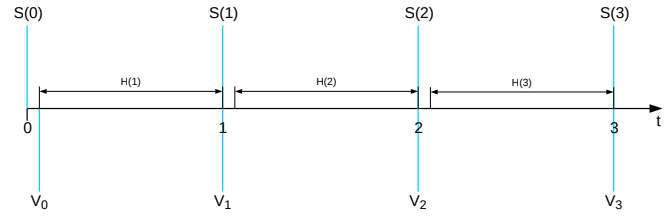
\includegraphics[width=.7\textwidth]{TradingStrategiesAndValueProcess.PNG}
    \caption{Diagram to show relationship between trading strategies $H$, values processes $V$ and stock processes $S$.}
    \label{fig_trading_strats_and_value_processes}
  \end{figure}

  \begin{definition}{Value Process $V$}
    The \textit{Value Process} $\{V_t\}_{t\in[0,T]}$ is a stochastic process defined by
    \[ V_t=\begin{cases}
      H_0(1)B_0+\sum_{n=1}^NH_n(1)S_n(0)&\text{if }t=0\\
      H_0(t)B_t+\sum_{n=1}^NH_n(t)S_n(t)&\text{if }t\geq1
    \end{cases} \]
    See \texttt{Figure \ref{fig_trading_strats_and_value_processes}}.
  \end{definition}

  \begin{definition}{Gains Process $G$}
    The \textit{Gains Process} $\{G_t\}_{t\in[0,T]}$ of a \textit{Trading Strategy} $H$ is given by
    \[ G_t=\left(\sum_{u=1}^tH_0(u)\Delta B_u\right)+\sum_{n=1}^N\sum_{u=1}^tH_n(u)\Delta S_n(u)\text{ where }\Delta S_n(t):=S_n(t)-S_n(t-1)\text{ for }t\geq1 \]
    This is an example of a stochastic integral of the trading strategy $H$ wrt to the price process $S$.
  \end{definition}

  \begin{definition}{Self-Financing Trading Strategies}
    A \textit{Trading Strategy} $H$ is \textit{Self-Financing} if
    \[ V_t=H_0(t+1)B_t+\sum_{n=1}^NH_n(t+1)S_n(t) \]
    You cannot introduce money into or take money out of a \textit{Self-Financing Trading Strategy} at any time-points $t$, except the first $t=0$ and last $t=T$.
  \end{definition}

  \begin{definition}{Discounted Processes $S_n^*,V^*$}
    The \textit{Discounte3d Price Process} $S_n^*=\{S_n^*(t)\}_{t\in[0,T]}$ for $n\in[1,N]$ is defined as
    \[ S_n^*(t)=\frac{S_n(t)}{B_t} \]
    The \textit{Discounted Value Process} $V^*=\{V_t^*\}_{t\in[0,T]}$ is defined as
    \[ V_t^*=\begin{cases}
      H_0(1)+\sum_{n=1}^nH_n(1)S_n^*(0)&\text{if }t=0\\
      H_0(t)+\sum_{n=1}^nH_n(t)S_n^*(t)&\text{if }t\geq1
    \end{cases} \]
    The \textit{Discounted Gains Process} $\{G_t^*\}_{t\in[1,T]}$ is defined as
    \[ G_t^*=\sum_{n=1}^N\sum_{u=1}^tH_n(u)\Delta S_n^*(u)\text{ for }t\geq1 \]
  \end{definition}

  \begin{proposition}{Self-Financing Trading Strategy and Value Process}\label{the_self_financing_and_value_process}
    A \textit{Trading Strategy} $H$ is \textit{Self-Financing} \underline{iff} $V_t^*=V_0^*+G_t^*$ for $t=1,\dots,T$.
  \end{proposition}

  \begin{proof}{\texttt{Proposition \ref{sec_multi_period_models}.\ref{the_self_financing_and_value_process}}}\label{proof_self_financing_and_value_process}
    For all $t=1,\dots,T$ it holds that
    \[ G_t^*=G_{t-1}^*+\sum_{n=1}^NH_n(t)\Delta S_n^*(t) \]
    For convenience we define $G_0^*=0$.
    \par I prove the statement in both directions
    \begin{itemize}
      \item[$\Longrightarrow$] Assume that $H$ is \textit{Self-Financing}.
      \par By the definitions of \textit{Self-Financing}, \textit{Discounted Processes} and the above result, we can show the following for all $t=1,\dots,T$
      \[\begin{array}{rcl}
        V_t^*-G_t^*&=&H_0(t)+\left(\sum_{n=1}^NH_n(t)S_n^*(t)\right)-\left(\sum_{n=1}^NH_n(t)\Delta S_n^*(t)\right)-G_{t-1}^*\\
        &=&H_0(t)+\left(\sum_{n=1}^NH_n(t)(S_n^*(t)-\Delta S_n^*(t))\right)-G_{t-1}^*\\
        &=&H_0(t)+\left(\sum_{n=1}^NH_n(t)S_n^*(t-1)\right)-G_{t-1}^*\\
        &=&V_{t-1}^*-G_{t-1}^*
      \end{array}\]
      By recursion we find that $V_t^*-G_t^*=V_0^*$.

      \item[$\Longleftarrow$] Assume that $V_t^*=V_0^*+G_t^*$ for all $t=1,\dots,T$.
      \par Then, for all $t=1,\dots,T_1$ we have the following
      \[\begin{array}{rcl}
        V_t^*-V_{t+1}^*&=&V_0^*+G_t^*-(V_0^*+G_{t+1}^*)\\
        &=&G_t^*-G_{t-1}^*
      \end{array}\]
      Therefore, by the definitions of discounted process and the result at the start of this proof
      \[\begin{array}{rcl}
        V_t^*&=&V_{t+1}^*-(G_{t+1}^*-G_t^*)\\
        &=&H_0(t+1)+\sum_{n=1}^NH_n(t+1)S_n^*(t+1)-\sum_{n=1}^NH_n(t+1)\Delta S_n^*(t+1)\\
        &=&H_0(t+1)+\sum_{n=1}^NH_n(t+1)
      \end{array}\]
      Thus $H$ is \textit{Self-Financing}.
    \end{itemize}
  \end{proof}

\subsection{Arbitrage in Multi-Period Model and Martingale Measures}

  \begin{example}{}
    \everymath={\displaystyle}
    Consider a model with $N=1$ stocks over $T=2$ time-periods and $K=4$ possible states.
    \par For simplicity we change the notation of the price process to $S_t$ instead of $S_1(t)$. The process is given by the following table
    \begin{center}
      $S_t(\omega)=$
      \begin{tabular}{c|ccc}
        $\omega\setminus t$&0&1&2\\\hline
        $\omega_1$&6&9&10\\
        $\omega_2$&6&9&7\\
        $\omega_3$&6&3&7\\
        $\omega_4$&6&3&1
      \end{tabular}
    \end{center}
    We further assume that the interest-rate $r$ is constant in both periods. Therefore the bank account process is $B_t=(1+r)^t$.
    \par The filtration generated by this price process is
    \[\begin{array}{rcl}
      \mathcal{F}_0&=&\big\{\emptyset,\Omega\big\}\\
      \mathcal{F}_1&=&\big\{\emptyset,\{\omega_1,\omega_2\},\{\omega_3,\omega_4\},\Omega\big\}\\
      \mathcal{F}_2&=&\big\{\emptyset,\{\omega_1\},\{\omega_2\},\{\omega_3\},\{\omega_4\},\{\omega_1,\omega_2\},\{\omega_1,\omega_3\},\{\omega_1,\omega_4\},\{\omega_2,\omega_3\},\{\omega_3,\omega_4\},\{\omega_3,\omega_4\},\\
      &&\{\omega_1,\omega_2,\omega_3\},\{\omega_1,\omega_2,\omega_4\},\{\omega_1,\omega_3,\omega_4\},\{\omega_2,\omega_3,\omega_4\},\Omega\big\}
    \end{array}\]
    Recall that the trading strategy has components $H_n(t)(\omega)$ giving the number of units of a stock held between time periods $t-1$ and $t$.
    \par Let $H$ be an arbitrary trading strategy, then for the value process for this problem we have
    \[ V_0(\omega)=H_0(1)(\omega)+6H_1(1)(\omega) \]
    Further
    \[\begin{array}{rcl}
      V_1(\omega)&=&\begin{cases}
        (1+r)H_0(1)(\omega)+9H_1(1)(\omega)&\text{if }\omega\in\{\omega_1,\omega_2\}\\
        (1+r)H_0(1)(\omega)+3H_1(1)(\omega)&\text{if }\omega\in\{\omega_3,\omega_4\}
      \end{cases}\\
      V_2(\omega)&=&\begin{cases}
        (1+r)^2H_0(2)(\omega)+10H_1(2)(\omega)&\text{if }\omega=\omega_1\\
        (1+r)^2H_0(2)(\omega)+7H_1(2)(\omega)&\text{if }\omega\in\{\omega_2,\omega_3\}\\
        (1+r)^2H_0(2)(\omega)+1H_1(2)(\omega)&\text{if }\omega=\omega_4
      \end{cases}
    \end{array}\]
    The \textit{Trading Strategy} $H$ is \textit{Predictable} so $H_i(1)(\omega)$ is constant for all $\omega$,
    $H_i(2)(\omega_1)=H_i(2)(\omega_2)$ and $H_i(2)(\omega_3)=H_i(2)(\omega_4)$.
    \par Now consider the gains process in this model
    \[ G_1(\omega)=\begin{cases}
      rH_0(1)+3H_1(1)&\text{if }\omega\in\{\omega_1,\omega_2\}\\
      rH_0(1)-3H_1(1)&\text{if }\omega\in\{\omega_3,\omega_4\}\\
    \end{cases} \]
    For brevity, we write $H_n(t)$ instead of $H_n(t)(\omega)$
    \[ G_2(\omega)=\begin{cases}
      rH_0(1)+3H_1(1)+r(1+r)H_0(2)+H_1(2)&\text{if }\omega=\omega_1\\
      rH_0(1)+3H_1(1)+r(1+r)H_0(2)-2H_1(2)&\text{if }\omega=\omega_2\\
      rH_0(1)-3H_1(1)+r(1+r)H_0(2)+4H_1(2)&\text{if }\omega=\omega_3\\
      rH_0(1)-3H_1(1)+r(1+r)H_0(2)-2H_1(2)&\text{if }\omega=\omega_4
    \end{cases} \]
    For the \textit{Trading Strategy} $H$ to be \textit{Self-Financing}, we must have that at time-point $t=1$ in states $\omega_1,\omega_2$
    \[ V_1=(1+r)H_0(1)+9H_1(1)=\footnotemark(1+r)H_0(2)+9H_1(2) \]
    \footnotetext{Condition for $H$ to be \textit{Self-Financing}.}
    In states $\omega_3,\omega_4$ we require
    \[ V_1=(1+r)H_0(1)+3H_1(1)=\footnotemark(1+r)H_0(2)+3H_1(2) \]
    \footnotetext{Condition for $H$ to be \textit{Self-Financing}.}
    We consider possible arbitrage opportunities without considering the existence of martingale measures for the moment. If the interest rate is $r=1/9$, then a possible trading strategy is as follows
    \begin{itemize}
      \item Start with an amount of £0.
      \item If $S_1=3$ do nothing at time points $t=0,1$.
      \item If $S_1=9$ at time point $t=1$ short sell one share of the risky asset ($H_1(2)=-1$) and put the received proceeds into the bank account ($H_0(2)=9/(1+r)$).
      \item Then, at time-point $t=2$ the value of the portfolio is
      \[ V_2=\begin{cases}
        (1+r)^2H_0(2)+10H_1(2)=10-10=0&\text{if }\omega=\omega_1\\
        (1+r)^2H_0(2)+7H_1(2)=10-7>0&\text{if }\omega=\omega_2\\
        0&\text{if }\omega\in\{\omega_3,\omega_4\}\end{cases} \]
    \end{itemize}
    If, on the other-hand, $r=0$ then there are no arbitrage opportunities.
    \par We now consider two ways to compute an equivalent martingale measure.
    \begin{enumerate}
      \item
      \par Recall that \texttt{Definition \ref{sec_multi_period_models}.\ref{def_martingale_measure}} states that
      \[ \expect_\Q\left[\frac{S_n(t+s)}{B_{t+s}}\bigg|\mathcal{F}_t\right]=\frac{S_n(t)}{B_t}\ \forall\ t,s\geq0 \]
      Let $q_i:=\Q(\{\omega_i\})$ for $i=1,2,3,4$. Further, we know that $q_1+q_2+q_3+q_4=1$ must hold and from the above result we have that
      \[\begin{array}{rrcl}
      (t=0,s=1)\implies&6(1+r)&=&9(q_1+1_2)+3(q_3+q_4)\\
      (t=0,s=2)\implies&6(1+r)^2&=&10q_1+7q_2+7q_3+q_4\\
      (t=1,s=1)\implies&9(1+r)&=&(10q_1+7q_2)/(q_1+q_2)\\
      (t=1,s=1)\implies&3(1+r)&=&(7q_3+q_4)/(q_3+q_4)
      \end{array}\]
      This gives five equations with four unknowns which could be solved to find $\Q$.

      \item We can make calculations quicker by considering conditional probabilities.
      \par At time $t=0$ we can obtain $p_1:=\Q(S_1=9)$ by solving
      \[ 6(1+r)=9p_1+3(1-p_1) \]
      Which produces that $\Q(S_1=9)=\frac{1+2r}2$ and $\Q(S_1=3)=\frac{1-2r}2$.
      \par At time $t=1$ is $\omega\in\{\omega_1,\omega_2\}$ we can write
      \[ p_2:=\Q(S_2=10|S_1=9)\text{ and }9(1+r)=10p_2+7(1-p_2) \]
      This produces that $\Q(S_2=10|S_1=9)=(2+9r)/3$ and $Q(S_2=7|S_1=9)=(1-9r)/3$.
      \par At time $t=1$ if $\omega\in\{\omega_3,\omega_4\}$ we can solve
      \[ p_3:=\Q(S_2=7|S_1=3)\text{ and }3(1+r)=7p_3+(1-p_3) \]
      to find that $\Q(S_2=7|S_1=3)=(2+3r)/6$ and $\Q(S_2=1|S_1=3)=(4-3r)/6$.
      \par By multiplying and conditional probabilities along the path leading to all four states in $\Omega$, we obtain
      \[\begin{array}{rcl}
        \Q(\{\omega_1\})&=&\frac{1+2r}2\cdot\frac{2-9r}3=\frac16(1+2r)(2+9r)\\
        \Q(\{\omega_2\})&=&\frac{1+2r}2\cdot\frac{1-9r}3=\frac16(1+2r)(1-9r)\\
        \Q(\{\omega_3\})&=&\frac1{12}(1-2r)(2+3r)\\
        \Q(\{\omega_4\})&=&\frac1{12}(1-2r)(4-3r)
      \end{array}\]
      All these probabilities are greater than 0 if $r<1/9$, thus we can conclude that a \textit{Martingale Measure} exists \underline{iff} $r\in[0,1/9)$.
    \end{enumerate}
  \end{example}

  \begin{definition}{Arbitrage Opportunity - Muliti-Period Model}
    An \textit{Arbitrage Opportunity} in the case of a multi-period model is a \textit{Trading Strategy} $H$ st
    \begin{enumerate}
      \item $V_0=0$ - It starts with zero money.
      \item $V_T\geq0$ - It does note loose money at the end.\footnote{It is possible for $V_t<0$ for $t\in(0,T)$.}
      \item $\expect[V_T]>0$ - It is expect that you always make money; And,
      \item $H$ is \textit{Self-Financing}.
    \end{enumerate}
  \end{definition}

  \begin{proposition}{Self-Financing Strategies and Arbitrage Opportunity}
    A \textit{Self-Financing Strategy} $H$ is an \textit{Arbitrage Opportunity} \underline{iff} all the following hold
    \[ G_T^*\geq0\quad\expect[G_T^*]>0\quad V_0^*=0 \]
  \end{proposition}

  \begin{definition}{Martingale Measure $\Q$}\label{def_martingale_measure}
    A \textit{Martingale Measure} is a probability measure $\Q$ st\footnote{This is similar to a \textit{Risk-Neutral Probability Measure}.}
    \begin{enumerate}
      \item $\Q(\{\omega\})>0\ \forall\ \omega\in\Omega$; and,
      \item The \textit{Discounted Price Process} $S_n^*$ is a \textit{Martingale} under $\Q$ for every $n=1,\dots,N$
      \[ \expect_\Q\left[S_n^*(t+s)|\mathcal{F}_t\right]=S_n^*(t)\ \forall\ t,s\geq0 \]
      More precisely, a \textit{Martingale Measure} $\Q$ must satisfy
      \[ \expect_\Q[S_n(t+s)/B_{t+s}|\mathcal{F}_t]=S_n(t)\ \forall\ t,s\geq0 \]
    \end{enumerate}
  \end{definition}

  \begin{theorem}{Extension of No-Arbitrage Principle}\label{the_extension_of_no_arbitrage_principle}
    There are no \textit{Arbitrage Opportunities} \underline{iff} there exists a \textit{Martingale Measure} $\Q$.\footnote{This is an extension of the ``No-Arbitrage Principle'' from the single-period model to the multi-period model.}
  \end{theorem}

  \begin{proposition}{Finance Processes which are Martingales\footnote{This proposition is useful for proving the Extension of No-Arbitrage Principle}}\label{prop_finance_processes_which_are_martingales}
    If $\Q$ is a \textit{Martingale Measure} and $H$ is a \textit{Self-Financing Strategy} then
    \begin{enumerate}
      \item The \textit{Discounted Value Process} $V^*$, and
      \item The \textit{Discounted Gains Process} $G^*$
    \end{enumerate}
    are \textit{Martingales} under $\Q$.
  \end{proposition}

  \begin{proof}{\texttt{Theorem \ref{sec_multi_period_models}.\ref{prop_finance_processes_which_are_martingales}}}
    \everymath={\displaystyle}
    We have to show that $\expect_\Q\left[V_{t+1}^*|\mathcal{F}_t\right]=V_t^*\ \forall\ t>0$.
    \par This is equivalent to showing that $\expect_\Q[G_{t+1}^*|\mathcal{F}_t]=G_t^*$ using \texttt{Proposition \ref{sec_multi_period_models}.\ref{the_self_financing_and_value_process}}.
    \par Using the expression for $G_{t+1}^*-G_t^*$ derived in \texttt{Proof \ref{sec_multi_period_models}.\ref{proof_self_financing_and_value_process}} we can conclude that
    \[\begin{array}{rcl}
      \expect_\Q\left[G_{t+1}^*-G_t^*|\mathcal{F}_t\right]&=&\expect_\Q\left[\sum_{n=1}^NH_n(t+1)\Delta S_n^*(t+1)\bigg|\mathcal{F}_t\right]\\
      &=&\sum_{n=1}^N\expect_\Q\big[\underbrace{H_n(t+1)}_{\in\mathcal{F}_t\footnotemark}\Delta S_n^*(t+1)|\mathcal{F}_t\big]\\
      &=&\sum_{n=1}^NH_n(t+1)\expect_\Q\left[\Delta S_n^*(t+1)|\mathcal{F}_t\right]
    \end{array}\]
    \footnotetext{This is due to $H_n(t+1)$ being the strategy we are building for time-step $t+1$ and thus we use all the information available in time-step $t$.}
    The last result is due to $H_n$ being a \textit{Trading Strategy} and thus \textit{Predictable}.
    \par Furthermore, $\expect_\Q\left[\Delta S_n^*(t+1)|\mathcal{F}_t\right]=$ for all $t>0$ since $S_n^*$ is a under $\Q$.
    \par Hence $G_t^*,V_t^*$ are \textit{Martingales}.\proved
  \end{proof}

  \begin{proposition}{Arbitrage Opportunities between Single-Period and Multi-Period Models}\label{prop_arbitrage_opportunities_single_and_multi_period_model}
    If the multi-period model does \underline{not} have any arbitrage opportunities, then all of the underlying single period model \underline{have} arbitrage opportunities.
  \end{proposition}

  \begin{proof}{\texttt{Proposition \ref{sec_multi_period_models}.\ref{prop_arbitrage_opportunities_single_and_multi_period_model}}}
    For each $t<T$ and for each $A\in\mathcal{P}_t$ there is one underlying single-period model where
    \begin{itemize}
      \item \textit{Initial Time Discounted Price} is $S_n^*(t,\omega)$ for an arbitrary $\omega\in A$ since $S_n^*(t,\omega)$ are constant on $A$.
      \item \textit{Sample Space} contains one state for each cell $A'\in\mathcal{P}_{t+1}$ st $A'\subset A$.
      \item \textit{Terminal Time Discounted Price} is $S_n^*(t+1,\omega)$ for each $n=1,\dots,N$ for some $\omega\in A$.
    \end{itemize}
    If any underlying single-period model has an arbitrage opportunity in the single-period sense, then the multi-period model must have an arbitrage opportunity in the multi-period sense.
    \par To see this, suppose there exists an \textit{Arbitrage Opportunity} $\hat{H}$ for the single period model corresponding to some $A\in\mathcal{P}_t$ for $t<T$. This means that the discounted gain, given as
    \[ \hat{H}_1\Delta S_n^*(t+1)+\dots+\hat{H}_N\Delta S_N^*(t+1) \]
    , is \textit{non-negative} and \underline{not} identical to zero on the event $A$.
    \par We now construct a multi-period \textit{Trading Strategy} $H$ which is an \textit{Arbitrage Opportunity}.
    \[ H_n(s,\omega)=\begin{cases}
      0&\text{if }s\leq t\text{ or }\omega\not\in A\\
      \hat{H}_n&\text{if }s=t+1,\ \omega\in A\text{, and }n=1,\dots,N\\
      -\sum_{i=1}^N\hat{H}_iS_i^*(t)&\text{if }s=t+1,\ \omega\in A\text{ and }n=0\\
      \sum_{i=1}^N\hat{H}_1\Delta S_1^*(t+1)&\text{if }s>t+1,\ \omega\in A\text{ and }n=0\\
      0&\text{if }s>t+1,\ \text{ and }n=0\\
    \end{cases} \]
    This strategy starts with zero money and does nothing unless the event $A$ occurs at time $t$, in which case at time $t$ the position $\hat{H}_n$ is taken in the $n^{th}$ risky security while the position in the bank account is used to self-finance.
    \par Subsequently, no position is taken in any of the risky securities, and non-zero value of the portfolio is reflected by a position in the bank account.
    \par THis \textit{Trading Strategy} $H$ is an \textit{Arbitrage Opportunity} in the multi-period model.\proved
  \end{proof}

  \begin{proof}{\texttt{Theorem \ref{sec_multi_period_models}.\ref{the_extension_of_no_arbitrage_principle}}}
    \begin{itemize}
      \item[$\longleftarrow$] We first show that there can be \underline{no} \textit{Arbitrage Opportunities} provided the existence of a \textit{Martingale Measure} $\Q$.
      \par Suppose $H$ is any \textit{Self-Finacing Trading Strategy} with
      \[ V_T^*\geq0\text{ and }\expect[V_T^*]>0 \]
      This implies
      \[ \expect_\Q[V_T^*]>0 \]
      Since $V^*$ is a \textit{Martingale} under $\Q$ by \texttt{Theorem \ref{sec_multi_period_models}.\ref{prop_finance_processes_which_are_martingales}}, it follows that
      \[ V_0^*=\expect_\Q[V_T^*]>0 \]
      Hence $H$ cannot be an \textit{Arbitrage Opportunity}, nor can any other trading strategies be \textit{Arbitrage Opportunities} due to $H$ being chosen arbitrarily.
      \item[$\longrightarrow$\footnote{This could be shown using a version of the \textit{Separating Hyperplane Theorem}, but it is easier to use results from the single-period model.}] Using \texttt{Proposition \ref{sec_multi_period_models}.\ref{prop_arbitrage_opportunities_single_and_multi_period_model}}, we have that for each $t<T$ and each $A\in\mathcal{P}_t$ there is a \textit{risk-neutral probability measure} $\Q(t,A)$ for the underlying single-period model.
      \par This probability measure gives positive mass to each cell $A'\in\mathcal{P}_{t+1}$ st it sums to 1 over all such cells and it satisfies
      \[ \expect_{\Q(t,A)}[\Delta S_n^*(t+1)]=0\text{ for }n=1,\dots,N \]
      Notice that $\Q(t,A)$ puts probability on each branch in the information tree which emerges from the node corresponding to $(t,A)$.
      \par We can calculate a \textit{Martingale Measure} $\Q$ for the multi-period model from these probabilities by setting $\Q(\{\omega\})$ equal to the product of the conditional probabilities along the path from the node at $t=0$ to the node at $(T,\omega)$.
      \par Then
      \begin{itemize}
        \item $\sum_{\omega\in\Omega}\Q(\{\omega\})=1$.
        \item $\Q(\{\omega\})>0$ for every $\omega\in\Omega$ because all the conditional risk neutral probabilities are strictly positive.
        \item And, $\expect_\Q[S_n^*(t+1)|\mathcal{F}_t]=S_n^*(t)$ for all $t$ and $n$.
      \end{itemize}
      Thus $\Q$ is indeed a \textit{Martingale Measure}.\proved
    \end{itemize}
  \end{proof}

\subsection{Valuation of Contingent Claims}

  \begin{definition}{Contingent Claim\footnote{This is an extension of \texttt{Definition \ref{sec_financial_terminology_and_single_period_model}.\ref{def_contingent_claim_single_period}} to the multi-period model.}}
    A \textit{Contingent Claim} in the multi-period model is a random variable $X$ which represents a payoff at the terminal time $t=T$.
    \par A \textit{Contingent Claim} $X$ is said to be \textit{Attainable}\footnote{AKA \textit{Marketable}.} if there exists a \textit{Self-Financing Trading Strategy} $H$ st $V_T(\omega)=X(\omega)\ \forall\ \omega\in\Omega$. In this case one says that $H$ ``generates'' $X$ and $H$ is called the \textit{Replicating Portfolio}.
  \end{definition}

  \begin{theorem}{Risk-Neutral Valuation Principle\footnote{This is an extension of \texttt{Theorem \ref{sec_financial_terminology_and_single_period_model}.\ref{the_risk_neutral_valuation_principle_single_period}} to the multi-period model.}}\label{the_risk_neutral_valuation_principle_multi_period}
    The time $t$ value of an \textit{Attainable Contingent Claim} $X$ is equal to $V_t$ where $V_t$ is the time $t$ value of the portfolio which replicates $X$.
    \par Moreover,
    \[ V_t^*=\frac{V_t}{B_t}=\expect_\Q[X/B_t|\mathcal{F}_t]\text{ for }t=0,\dots,T\text{ and all }\Q \]
  \end{theorem}

  \begin{proof}{\texttt{Theorem \ref{sec_multi_period_models}.\ref{the_risk_neutral_valuation_principle_multi_period}}}
    Let $P_t$ denote the actual price of the \textit{Contingent Claim} at time point $t$.
    \par By \texttt{Theorem \ref{sec_financial_terminology_and_single_period_model}.\ref{thrm_equivalent_contract_valuations_over_time}}, $P_t=V_t$ is the only possibility to avoid arbitrage opportunities.
    \par Now, let $\Q$ be an arbitrary \textit{Martingale Measure} then for every $t<T$ we have that
    \[ V_t^*:=\expect_\Q[V_t^*|\mathcal{F}_t] \]
    as $V_t^*$ is a \textit{Martingale} by \texttt{Proposition \ref{sec_multi_period_models}.\ref{prop_finance_processes_which_are_martingales}}.
    \par Moreover, since $V_T^*$ is the discounted value of the portfolio which replicated $X$ we have that
    \[ \expect_\Q[V_T^*|\mathcal{F}_t]=\expect_\Q[X/B_T|\mathcal{F}_t] \]
    Thus $V_t^*=\expect_\Q[X/B_T|\mathcal{F}_t]$ independent of the choice of \textit{Martingale Measure} $\Q$.
  \end{proof}

  \begin{remark}{Computing a Generating a Trading Strategy $H$}
    If we already know the \textit{Value Process} $\{V_t\}_{t\in\nats_0}$ for the replicating portfolio, we need to solve for the trading strategy $H$ using the linear equations in the definition of the value process (keeping in mind that $H$ is \textit{Predictable}).
    \[ V_t(\omega_i)=H_0(t)B_t+\sum_{n=1}^NH_n(t)S_n(t)(\omega_i)\ \forall\ \omega_i\in\Omega \]
    However, if we only know the \textit{Contingent Claim} $X$ we need to work backwards in time, deriving $V$ and $H$ simultaneously.
    \par Since $V_T=X$ we must first solve the following for $H(T)$.
    \[ X(\omega_i)=H_0(T)B)T+\sum_{n=1}^NH_n(T)S_n(T)(\omega_i) \]
    Since $H$ is self-financing, we can calculate $V_{T-1}$.
    \[ V_{T-1}=H_0(T)B_{T-1}+\sum_{n=1}^NH_n(T)S_n(T-1)(\omega_i) \]
    Therefore, our next step is to solve the following for $H(T_1)$.
    \[ V_{T-1}=H_0(T_1)B_{T-1}+\sum_{n=1}^NH_n(T-1)S_n(T-1)(\omega_i) \]
    We can now continue by calculating $V_{T-2}$ etc. until we end up with $V_0$.
  \end{remark}

  \begin{example}{Finding a Replicating Portfolio}
    Consider a European call option with exercise price $e=5$.
    \par The corresponding contingent claim is $X=\{S_2-5\}_+$ and takes the values $\{5,2,2,0\}$ in states $\{\omega_1,\omega_2,\omega_3,\omega_4\}$ respectively.
    \par Suppose $r=0$ then $\Q=(1/3,1/6,1/6,1/3)$.
    \par Since the martingale measure is unique, \texttt{Proposition \ref{sec_multi_period_models}.\ref{prop_complete_model_and_martingale_measures}} will show below that the model is complete and therefore every \textit{Contingent Claim} is \textit{Marketbale} (inc. the European option).
    \par At time $t=0$ the contingent claim's value must be
    \[ V_0=\expect_\Q[X]=(1/3)\cdot5+(1/6)\cdot2+(1/6)\cdot2+(1/3)\cdot0=7/3 \]
    At time $t=1$ the contingent claim's value in states $\omega_1,\omega_2$ is
    \[ V_1(\omega_1)=V_1(\omega_2)=\expect_\Q[X|S_1=9]=(2/3)\cdot5+(1/3)\cdot2=4 \]
    At time $t=1$ the contingent claim's value in states $\omega_3,\omega_4$ is
    \[ V_1(\omega_3)=V_1(\omega_4)=\expect_\Q[X|S_1=3]=(1/3)\cdot2+(2/3)\cdot0=2/3 \]
    To find a replicating portfolio we start at time $t=2$ and find that
    \[\begin{array}{rcl}
      V_2(\omega_1)&=&5=H_0(2)(\omega_1,\omega_2)\cdot B_2+H_1(2)(\omega_1,\omega_2)\cdot 10\\
      V_2(\omega_2)&=&2=H_0(2)(\omega_1,\omega_2)\cdot B_2+H_1(2)(\omega_1,\omega_2)\cdot 7
    \end{array}\]
    Noting that $B_2=1$, we obtain that $H_0(2)(\omega_1,\omega_2)=-5$ and $H_1(2)(\omega_1,\omega_2)=1$.
    \par Similarly
    \[\begin{array}{rcl}
      V_2(\omega_3)&=&2=H_0(2)(\omega_3,\omega_4)\cdot 1+H_1(2)(\omega_3,\omega_4)\cdot 7\\
      V_2(\omega_4)&=&0=H_0(2)(\omega_3,\omega_4)\cdot 1+H_1(2)(\omega_3,\omega_4)\cdot 1
    \end{array}\]
    and obtain that $H_0(2)(\omega_3,\omega_4)=-1/3$ and $H_1(2)(\omega_3,\omega_4)=1/3$.
    \par Now we have two ways to proceed
    \begin{enumerate}
      \item Since we have already calculated the value of the option at time-point $t=1$ we can proceed as in the second period.
      \par Writing $H_0(1)$ for $H_0(1)(\omega_1,\dots,\omega_4)$ and $H_1(1)$ for $H_1(1)(\omega_1,\dots,\omega_4)$, we have
      \[\begin{array}{rcrcl}
        V_1(\omega)&=&4&=&H_0(1)\cdot B_1+H_1(1)\cdot9\text{ for }\omega\in\{\omega_1,\omega_2\}\\
        V_1(\omega)&=&2/3&=&H_0(1)\cdot B_1+H_1(1)\cdot3\text{ for }\omega\in\{\omega_3,\omega_4\}
      \end{array}\]
      Solving these equations, and noting $B_1=1$, gives $H_0(1)=-1$ and $H_1(1)=5/9$.
      \par Note that this confirms our calculation for $V_0$, since this portfolio costs $-1+6(5/9)=7/3$ at time $t=0$.
      \item Suppose we had not already calculated the value of the option at time $t=1$.
      \par Using that $H$ is \textit{Self-Financing} we calculate the value of the portfolio at time-point $t=1$.
      \par So we assume that we have already calculated $H_0(2)$ and $H_1(2)$. Then
      \[ V_1=H_0(2)\cdot1+H_1(2)\cdot9=-5\cdot1+1\cdot9=4\text{ in }\omega_1,\omega_2 \]
      Similarly
      \[ V_1=(-1/3)\cdot1+(1/3)\cdot 3=2/3\text{ in }\omega_3,\omega_4 \]
      We proceed as above, obtaining
      \[ H_0(1)=-1\quad H_1(1)=5/9 \]
    \end{enumerate}
  \end{example}

  \begin{proposition}{Complete Markets and Martingale Measures}\label{prop_complete_model_and_martingale_measures}
    An arbitrage-free multi-period model is complete \underline{iff} there exists a unique martingale measure $\Q$.
  \end{proposition}

  \begin{proof}{\texttt{Proposition \ref{sec_multi_period_models}.\ref{prop_complete_model_and_martingale_measures}}}
    \begin{itemize}
      \item If the multi-period model is complete, for any claim $X$ we can work backwards in time to compute the trading strategy that generates $X$. Hence, for each underlying single-period model the matrix $A$ must have independent columns and the model is complete.
      \item Conversely, if every underlying single-period model is complete then the computational procedure for the multi-period model succeeds.
    \end{itemize}
    Therefore, completeness of the multi-period model is equivalent to completeness of all underlying single-period models.
    \par In particular the multi-period model is complete \underline{iff} each underlying model has a unique risk-neutral probability measure.
    \par On the other hand, uniqueness of the martingale measure $\Q$ is equivalent to uniqueness of the risk-neutral probability measures of the underlying single-period models.
    \par Obviously, the existence of several risk-neutral probability measures for a single-period model leads to several multi-period martingale measures.
    \par However, assume there are two multi-period martingale measures. Then the conditional probability must be different for at least one specific single-period model.\proved
  \end{proof}

\subsection{American Claims}

  \begin{definition}{American Claim $Y_\tau$}
    Let $\{Y_t\}_{t\in T}$ be a stochastic process describing the payoff of a financial derivative if exercised at time $t$ and let $\tau$ be the stopping time representing the exercise date in an \textit{Exercise Strategy}.
    \par Then $Y_\tau$ is called the \textit{American Claim} wrt to $Y_t$ and $\tau$.\footnote{Stopping times needs to be $\mathcal{F}_t$ measurable so we will know at time $t$ whether we will exercise the \textit{American Claim}.}
  \end{definition}

  \begin{definition}{Attainable American Claim}
    The \textit{American Claim} $Y_\tau$ is said to be \textit{Attainable}\footnote{AKA ``Marketable''} if there exists a \textit{Self-Financing Trading Strategy} $H$ st the corresponding portfolio value $V$ satisfies $V_\tau=Y_\tau$.
    \par An \textit{American Pay-off Process} $\{Y_t\}$ is said to be attainable if for every \textit{Stopping Time} $\tau$ the \textit{American Claim} $Y_\tau$ is \textit{Attainable}.
  \end{definition}

  \begin{proposition}{Complete Markets \& Attainable American Claims}\label{prop_complete_markets_and_attainable_american_claims}
    If a financial market is \textit{Complete} then \underline{every} \textit{American Claim} is \textit{Attainable}.
  \end{proposition}

  \begin{proof}{\texttt{Proposition \ref{sec_multi_period_models}.\ref{prop_complete_markets_and_attainable_american_claims}}}
    Let $\{Y_t\}_{t\in T}$ be a payoff-process and $\tau$ be an exercise strategy.
    \par  We have to find a self-financing trading strategy $H$ st $V_\tau=Y_\tau$.
    \par Consider the \textit{European Claim} $X=Y_\tau(B_T/B_\tau)$ which corresponds to someone exercising the \textit{American Claim} $Y$ at time-point $t=\tau$ and then earning interest from a bank-account until time-point $T$. Since the model is complete, there must be a replicating trading strategy $H$ st $V_T=X=Y_\tau(B_T/B_\tau)$.
    \par This portfolio which starts at time $\tau$ with the amount of $Y_\tau$ all of which is put into and kept in the bank account until time $T$, has the same value at time $T$ as $H$.
    \par We conclude that $V_\tau=Y_\tau$.\proved
  \end{proof}

  \begin{definition}{Snell Envelope}
    Let $\{X_t\}_{t\in T}$ be a stochastic process adapted to some filtration $\mathcal{F}_t$.
    \par Then the process $\{Z_t\}_{t\in T}$, defined below, is called the \textit{Snell Envelope} of $X$.
    \[ Z_t=\begin{cases}
      X_T&\text{if }t=T\\
      \max\{X_t,\expect[Z_{t+1}|\mathcal{F}_t]\}&\text{if }t<T
    \end{cases} \]
  \end{definition}

  \begin{example}{Snell Envelope}
    Consider rolling a six-sided die three times. After the $i^{th}$ roll, you can either keep the score $X_i$ on the die, or roll again. Whoever gets the highest score wins. What should your strategy be?
    \par First, note that we have to keep the third score if we roll the die three times. Moreover, after the second roll we take
    \[ Z_2=\max\{X_2,\expect[Z_3|\mathcal{F}_2]\}\footnotemark=\max\{X_2,\expect[X_3]\}=\max\{X_2,7/2\} \]
    \footnotetext{In this game $\mathcal{F}_t$ is not helpful as each roll is independent.}
    This means we should stick with the second roll if it is greater than or equal to 4, otherwise re-roll. Thus
    \[ \expect[Z_2]=\expect[\max\{X_2,7/2\}]=\frac16\cdot\left(\frac72+\frac72+\frac72+4+5+6\right)=\frac{17}4 \]
    After the first roll, we take
    \[ Z_1=\max\{X_1,\expect[Z_2|\mathcal{F}_1]=\max\{X_1,\expect[Z_2]\}=\max\left\{X_1,\frac{17}4\right\} \]
    This means we should stick with the first roll if it is greater than or equal to 5, otherwise re-roll.
  \end{example}

  \begin{theorem}{Snell Envelope is the Smallest Super-Martingale}\label{the_snell_envelope_super_martingale}
    The \textit{Snell Envelope} $\{Z_t\}$ of $X$ is the smallest \textit{Super-Martingale} which dominates $X$.
    \par (i.e. $Z_t\geq X_t\ \forall\ t$).
  \end{theorem}

  \begin{proof}{\texttt{Theorem \ref{sec_multi_period_models}.\ref{the_snell_envelope_super_martingale}}}
    First, $Z_t\geq\expect[Z_{t+1}|\mathcal{F}_t]$ and $Z_t\geq X_t$, so $\{Z_t\}$ is a super-martingale and dominates $X$.
    \par Next, let $\{U_t\}_{t\in T}$ be any other supermartinale which dominates $X$. Since, by definition, $Z_T=X_T$ and $U$ dominates $X$ we must have $U_T\geq Z_T$. Assume inductively that $U_t\geq Z_t$. Then
    \[\begin{array}{rcl}
      U_{t-1}&\geq&\expect[U_t|\mathcal{F}_{t-1}]\text{ since }U_t\text{ is a supermartingale}\\
      &\geq&\expect[Z_t|\mathcal{F}_{t-1}]
    \end{array}\]
    and $U$ dominates $X$
    \[ U_{t-1}\geq X_{t-1} \]
    Combining
    \[ U_{t-1}\geq\max\{X_{t-1}\expect[Z_t|\mathcal{F}_{t-1}] \]
    By repeating this argument we get $U_t\geq Z_t\ \forall\ t$.\proved
  \end{proof}

  \begin{proposition}{Snell Envelope as Discounted Value Process}\label{prop_snell_envelope_as_discounted_value_process}
    Consider a financial market with a \textit{Martingale Measure} $\Q$ and an attainable \textit{American Payoff Process} $\{Y_t\}$.
    \par Then the \textit{Snell Envelope} $\{Z_t\}$ of the discounted payoff process $\{Y_t/B_t\}$ is the discounted value process for $Y$.
  \end{proposition}

  \begin{proof}{\texttt{Proposition \ref{sec_multi_period_models}.\ref{prop_snell_envelope_as_discounted_value_process}}}
    % Prop 3.22
    \textit{This proof uses the Optimal Stopping Theorem (\texttt{Theorem \ref{sec_multi_period_models}.\ref{the_optimal_stopping_theorem}})}.
    \par Let $p$ denote the time $t$ price of the American claim wrt the payoff process $(Y_t/B_t)$.
    \par Suppose, first, that $p<Z_t$ then:
    \begin{itemize}
      \item We buy the option for $p$.
      \item If $\tau(t)=t$\footnote{This is unlikely as the arbitrage opportunity is obvious.} then $Z_t=Y_t/B_t$ and so we can exercise the option immediately for $(Y_t/B_t)>p$ to make a riskless profit.
      \item If $\tau(t)>t$ we undertake the negative of the trading strategy that replicates $Y_{\tau(t)}/B_{\tau(t)}$, as we want to short sell. The price of the replicating strategy is $\expect_Q[Y_{\tau(t)}/B_{\tau(t)}|\mathcal{F}_t]$ by the \textit{Risk-Netural Valuation Principle} (\texttt{Theorem \ref{sec_multi_period_models}.\ref{the_risk_neutral_valuation_principle_multi_period}}), but by the \textit{Optimal Stopping Theorem} (\texttt{Theorem \ref{sec_multi_period_models}.\ref{the_optimal_stopping_theorem}}) this is equal to $Z_t$ and so we can invest the different $Z_t-p$ in the bank account.
      \item Later at time $\tau(t)$ we exercise the option and liquidate the replicating portfolio at the same time. The amount we collect from the option seller is equal to our liability on the portfolio\footnote{Meaning the cash flow at this time-period is net 0}. Meanwhile, we have $(Z_t-p)\cdot(B_{\tau(t)}/B_t)>0$ in the bank account.
    \end{itemize}
    This shows that we make a riskless profit in any case.

    \par Now consider the case where $p>Z_t$ then
    \begin{itemize}
      \item We sell the option for $p$.
    \end{itemize}
    Consider in detail the case where $\tau(t)>t$. Then
    \begin{itemize}
      \item We undertake the trading strategy that replicates $Y_{\tau(t)}/B_{\tau(t)}$. Again we find by using \textit{Risk-Netural Valuation Principle} (\texttt{Theorem \ref{sec_multi_period_models}.\ref{the_risk_neutral_valuation_principle_multi_period}}) and the \textit{Optimal Stopping Theorem} (\texttt{Theorem \ref{sec_multi_period_models}.\ref{the_optimal_stopping_theorem}}) that the price of building up the portfolio is
      \[ Z_t=\expect_\Q[Y_{\tau(t)/B_{\tau(t)}}|\mathcal{F}_t] \]
      \item Therefore there is a profit of $p-Z_t$ which we put in the bank account.
    \end{itemize}
    How we proceed will depend on when the buyer exercises the option.
    \begin{enumerate}
      \item If the buyer exercises the option at time-point $s\leq\tau(t)$ then
      \begin{itemize}
        \item We pay the buyer the payoff $Y_s/B_s$.
        \item We liquidate our portfolio and using risk-neutral valuation the value of our portfolio at time-point $s$ is
        \[ \expect_\Q[Y_{\tau(t)}/B_{\tau(t)}|\mathcal{F}_s] \]
        Since $s\in[t,\tau(t)]$ we see from the definition of $\tau(t)$ that $\tau(t)=\tau(s)$.
        \par Using this and the \textit{Optimal Stopping Theorem} (\texttt{Theorem \ref{sec_multi_period_models}.\ref{the_optimal_stopping_theorem}}) that the value of our portfolio at time $s$ is
        \[ \expect_\Q[Y_{\tau(t)}/B_{\tau(t)}|\mathcal{F}_s]=\expect_\Q[Y_{\tau(s)}/B_{\tau(s)}|\mathcal{F}_s]=Z_s\geq (Y_s/B_s) \]
        \item Therefore all transaction at time-point $s$ will only add to our portfolio and our total profit is strictly positive.
      \end{itemize}
      \item If the buyer does not exercise by time $s=\tau(t)$ where $\tau(t)<T$ then:
      \begin{itemize}
        \item We repeat the process, undertaking the trading strategy that replicates $Y_{\tau(s+1)}/B_{\tau(s+1)}$.
        \item The value of the portfolio to be built up is equal to
        \[ \expect_\Q[Y_{\tau(s+1)}/B_{\tau(s+1)}|\mathcal{F}_s]\leq\expect_\Q[Y_{\tau(s)}/B_{\tau(s)}|\mathcal{F}_s]=Z_s \]
        Therefore the change of the portfolio will only pay us some money which we put in the bank account.
        \item As before, if the option buyer exercises at some time $u\leq\tau(s+1)$ then the value of the portfolio will be enough to cover the payoff $Y_u$.
      \end{itemize}
      \item If the buyer has not exercised by time $\tau(s+1)$ then we repeat this process again, and so forth. There will always be enough money in the portfolio to cover the payoff. Our overall profit will be at least $p-Z_t>0$/
    \end{enumerate}
    Finally, we consider the case where $\tau(t)$. Then the optimal strategy would be to exercise the option immediately.
    \begin{itemize}
      \item If the buyer indeed exercises at time $t$, then we pay them $(Y_t/B_t)=Z_t<p$ and make a riskless-profit.
      \item If note, then we proceed as in the previous case where the buyer does not exercise by the optimal stopping time and undertake the trading strategy which replicates $(Y_{\tau(t+1)}/B_{\tau(t+1)})$ and so forth making again profit of at least $p-Z_t$.
    \end{itemize}
    \proved
  \end{proof}

  \begin{theorem}{Optimal Stopping Theorem}\label{the_optimal_stopping_theorem}
    \textit{This is \underline{NOT} the ``Optional Stopping Theorem'' (\texttt{Theorem \ref{sec_stochastic_processes_in_discrete_time}.\ref{the_optional_sampling_theorem}})}.
    \par Let $\{X_t\}_{t\in T}$ be a stochastic process adapted to some \textit{Filtration} $\mathcal{F}_t$ and $Z_t$ be the \textit{Snell Envelope} of $\{X_t\}_{t\in T}$.
    \par For any $t=0,\dots,T$ we define a stopping time by $\tau(t)=\min_{s\geq t}\{Z_s=X_s\}$, then the optimal stopping rule is
    \begin{equation}\label{eq_optimal_stopping_rule}
      Z_t=\expect[X_{\tau(t)}|\mathcal{F}_t]=\max_t\left\{\expect[X_{\tau}|\mathcal{F}_t]:\text{ all stopping times }t\leq\tau\leq T\right\}\text{ for all }t=0,\dots,T
    \end{equation}
    In particular
    \[ Z_0=\expect[X_{\tau(0)}]=\max_t\left\{\expect[X_{\tau)}|\mathcal{F}_t]:\text{ all stopping times }\tau\leq T\right\} \]
  \end{theorem}

  \begin{proof}{\texttt{Theorem \ref{sec_multi_period_models}.\ref{the_optimal_stopping_theorem}}}
    \textit{This proof is a backwards induction through time}.
    \par \underline{Base Case}
    \par Note first that  \texttt{Eq. \ref{eq_optimal_stopping_rule}} is clearly true for $t=T$ because, by definition of the \textit{Snell Envelope}, $Z_T=X_T$ and therefore the stopping time $\tau(T)$ stops at $T$.
    \par \underline{Inducitve Step}
    \par Now assume that \texttt{Eq. \ref{eq_optimal_stopping_rule}} is satisfied for some $t$, we now need to show it holds for $t-1$. Let $\tau$ be an arbitrary stopping time between $t-1$ and $T$.
    \par Define another stopping time $\tau'=\max\{\tau,t\}$\footnote{This is similar to $\tau$ but can never take the value $t-1$.}. Then, since $\tau\geq t\implies\ \tau'=\tau$
    \[\begin{array}{rcl}
      \expect[X_\tau|\mathcal{F}_{t-1}]&=&\expect[\indexed\{\tau=t-1\}X_{t-1}+\indexed\{\tau>t-1\}X_\tau|\mathcal{F}_{t-1}]\\
      &=&\expect[\indexed\{\tau=t-1\}X_{t-1}+\indexed\{\tau>t-1\}X_{\tau'}|\mathcal{F}_{t-1}]\\
      &=&\indexed\{\tau=t-1\}X_{t-1}+\indexed\{\tau>t-1\}\expect[X_{\tau'}|\mathcal{F}_{t-1}]\\
      &=&\indexed\{\tau=t-1\}X_{t-1}+\indexed\{\tau>t-1\}\expect[\expect[X_{\tau'}|\mathcal{F}_t]|\mathcal{F}_{t-1}]\text{ by Tower Law}
    \end{array}\]
    Since $\tau'$ is a stopping time st $\tau'\in[t,T]$, we find that $\expect[X_{\tau'}|\mathcal{F}_t]\leq Z_t$ because we have assumed \texttt{Eq. \ref{eq_optimal_stopping_rule}} holds for $t$.
    \par Using the definition of $Z_{t-1}$ we see that
    \[\begin{array}{rcl}
      \expect[X_\tau|\mathcal{F}_{t-1}]&\leq&\indexed\{\tau=t-1\}X_{t-1}+\indexed\{\tau>t-1\}\expect[Z_t|\mathcal{F}_{t-1}]\\
      &\leq&Z_{t-1}\text{by def. Snell Envelope}
    \end{array}\]
    In the special case where $\tau=\tau(t-1)$ we find that $\tau=(t-1)$ stops in $t-1$ \underline{iff} $Z_{t-1}=X_{t-1}$, otherwise $Z_{t-1}>X_{t-1}$\footnote{As $\{Z_t\}$ dominates $\{X_t\}$.} and $\tau(t-1)=\tau(t)$. Hence
    \[\begin{array}{rcl}
      \expect[X_{\tau(t-1)}|\mathcal{F}_{t-1}]&=&\indexed\{Z_{t-1}=X_{t-1}\}X_{t-1}+\indexed\{Z_{t-1}>X_{t-1}\}\expect[\expect[X_{\tau(t)}|\mathcal{F}_t]|\mathcal{F}_{t-1}]\\
      &=&\indexed\{Z_{t-1}=X_{t-1}\}X_{t-1}+\indexed\{Z_{t-1}>X_{t-1}\}\expect[Z_t|\mathcal{F}_{t-1}]\\
      &=&Z_{t-1}\text{ by def. Snell Envelope}
    \end{array}\]
  \end{proof}

  \begin{example}{Snell Envelope - \#1}\label{ex_snell_evelope_1}
    Consider a market where there is a bank account with interest-rate $r=0$ and a single security with the following price process
    \begin{center}
      $S_t(\omega)=$\begin{tabular}{c|ccc}
        $\omega\setminus t$&0&1&2\\\hline
        $\omega_1$&6&9&10\\
        $\omega_2$&6&9&7\\
        $\omega_3$&6&3&7\\
        $\omega_4$&6&3&1
      \end{tabular}
    \end{center}
    For this model, $\Q(\omega):=(1/3,1/6,1/6,1/3)$ is a risk-neutral probability measure.
    \par Consider an American call option with the exercise price of £5. Then its payoff process is
    \begin{center}
      $Y_t(\omega)=$\begin{tabular}{c|ccc}
        $\omega\setminus t$&0&1&2\\\hline
        $\omega_1$&1&4&5\\
        $\omega_2$&1&4&2\\
        $\omega_3$&1&0&2\\
        $\omega_4$&1&0&0
      \end{tabular}
    \end{center}
    In states $\omega_3,\omega_4$ the price
    \[\begin{array}{rcl}
      Z_1&=&\max\{Y_1,\expect_\Q[Z_2|\mathcal{F}_1]\}\\
      &=&\max\{0,2\cdot(1/3)+0\cdot(2/3)\}\\
      &=&2/3
    \end{array}\]
    This is equal to the European Option above $V_1(\omega_3,\omega_4)$.
    \par In states $\omega_1,\omega_2$ the price
    \[\begin{array}{rcl}
      Z_1&=&\max\{Y_1,\expect_\Q[Z_2|\mathcal{F}_1]\}\\
      &=&\max\{4,5\cdot(2/3)+2\cdot(1/3)\}\\
      &=&4
    \end{array}\]
    This is equal to the European Option above $V_1(\omega_1,\omega_2)$.
    \par so $Z_0=\max\{1,(2/3)\cdot(1/2)+4\cdot(1/2)\}=7/3$. The time $t=0$ price of the European call option of
  \end{example}

  \begin{example}{Snell Envelope - \#2}
    Consider the same scenario as \texttt{Example \ref{sec_multi_period_models}.\ref{ex_snell_evelope_1}} except that the payoff process of the American call option is
    \begin{center}
      $Y_t(\omega)=$\begin{tabular}{c|ccc}
        $\omega\setminus t$&0&1&2\\\hline
        $\omega_1$&1&5&5\\
        $\omega_2$&1&5&2\\
        $\omega_3$&1&0&2\\
        $\omega_4$&1&0&0
      \end{tabular}
    \end{center}
    At time-point $t=2$ it still holds that $Z_2=Y_2$. Moreover, $\expect_\Q[Z_2|\mathcal{F}_1]=\expect_\Q[Y_2|\mathcal{F}_1]$ which is the same as \texttt{Example \ref{sec_multi_period_models}.\ref{ex_snell_evelope_1}}.
    \par So
    \[\begin{array}{rcl}
      \expect_Q[Z_2|\mathcal{F}_1]&=&\begin{cases}
        (2/3)\cdot5+(1/3)\cdot2&\text{if in }\omega_1,\omega_2\\
        (1/3)\cdot2+(2/3)\cdot0&\text{if in }\omega_3,\omega_4
      \end{cases}\\
      &=&\begin{cases}
        4&\text{if in }\omega_1,\omega_2\\
        2/3&\text{if in }\omega_3,\omega_4
      \end{cases}
    \end{array}\]
    Hence
    \[\begin{array}{rcl}
      Z_1&=&\max\{Y_1\expect_\Q[Z_2|\mathcal{F}_1]\\
      &=&\begin{cases}
        \max\{4,5\}=5&\text{if in }\omega_1,\omega_2\\
        \max\{0,2/3\}=5&\text{if in }\omega_3,\omega_4
      \end{cases}
    \end{array}\]
    For time $t=0$ we have
    \[\begin{array}{rcl}
      \expect_\Q[Z_1|\mathcal{F}_0]&=&\expect_\Q[Z_1]\\
      &=&(1/2)\cdot5+(1/2)\cdot(2/3)\\
      &=&17/6
    \end{array}\]
    in which case $Z_0=\max\{Y_0,\expect_\Q[Z_1]\}=17/6$.
    \par The optimal exercise strategies are
    \[ \tau(0)(\omega)=\tau(1)(\omega)=\begin{cases}
      1&\text{if in }\omega_1,\omega_2\\
      2&\text{if in }\omega_3,\omega_4
    \end{cases} \]
    and, of course, $\tau(2)(\omega)=2\ \forall\ \omega\in\Omega$.
    \par Finally, we compute a replicating trading strategy for $\tau(0)$.
    \par In states $\omega_3,\omega_4$ the stopping time $\tau(0)$ stops in time 2 so the portfolio in the second period must satisfy
    \[\begin{array}{rcl}
      H_0(2)+7\cdot H_1(2)&=&Y_2(\omega_3)=2\\
      H_0(2)+1\cdot H_1(2)&=&Y_2(\omega_4)=0
    \end{array}\]
    Let $H_i(2):=H_i(2)(\omega_3,\omega_4)$.
    \par Then the solution is that $H_0(2)=-1/3$ and $H_1(2)=1/3$ in states $\omega_3,\omega_4$.
    \par The value of this portfolio at time $t=1$ is $-(1/3)+3\cdot(1/3)=2/3$.
    \par The values of $H_0(2)$ and $H_1(2)$ in states $\omega_1,\omega_2$ do not matter.
    \par In the first period, the portfolio must satisfy
    \[\begin{array}{rcl}
      H_0(1)+9H_1(1)&=&Z_1(\omega_1)=Z_1(\omega_2)=5\\
      H_0(1)+3H_1(1)&=&Z_1(\omega_3)=Z_1(\omega_4)=2/3
    \end{array}\]
    which has solutions $H_0(1)=-3/2$ and $H_1(1)=13/18$.
    \par The American option is attainable with time $t=0$ value of $1\cdot(-3/2)+6\cdot(13/18)=17/6$ which confirms previous calculations\footnote{Showing this is a replicating portfolio.}.
  \end{example}

\subsection{The Cox-Ross-Rubinstein Model}

  \begin{definition}{Bernoulli Process}
    Let $\{X_t:t=1,2,\dots\},\ \{N_t:t=1,2,\dots\}$ be a \textit{Stochastic Process}.
    \par $\{X_t\}_t$ is a \textit{Bernoulli Process} with parameter $p$ if the random variable $X_1,X_2,\dots$ are independent and
    \[ \prob(X_t=1)=1-\prob(X_t=0)=p\ \forall\ t \]
    \par $\{N_t\}_t$ is a \textit{Random Walk Process} when $N_t:=X_1+\dots+X_t$ and $\{X_t\}_t$ is a \textit{Bernoulli Process}.
  \end{definition}

  \begin{definition}{Cox-Ross-Rubinstein Model\footnote{AKA ``Binomial Model''}}
    The \textit{Cox-Ross Rubinstein Model}\footnote{This simplifies a special case of the general multi-period model where prices move up and down by a fixed ratio and moves occur with fixed probability, wrt $t$.} consists of a bank account with constant interest rate $r>0$ and \underline{one} risky asset with price process $S_t$ defined by
    \[ S_t=S_0u^{N_t}d^{t-N_t}\text{ for }t=1,\dots,T \]
    Here $N_t=X_1+\dots+X_t$ is the \textit{Random Walk Process} associated with a \textit{Bernoulli Process} $X_t$ associated with a \textit{Bernoulli Process} $X_t$ with parameter $p\in(0,1)$; $u$ is the ratio of the price after it has increases\footnote{$u=S_{t+1}/S_t$ when $S_{t+1}>S_t$. $u$ is constant for all $t$.}; $d$ is the ratio of the price after it has decreased; and $S_0$ is the start price.
    \par Note $u,d,S_0$ are all positive real values and in well-defined models $0<d<1<u$.
  \end{definition}

  \begin{remark}{Events in Cox-Ross-Rubinstein Model}
    In each time-period, two events are possible under the \textit{Cox-Ross-Rubinstein Model}
    \begin{enumerate}
      \item Price increases by a factor of $u$. This occurs with probabilty $p$.
      \item Price decreases by a factor of $d$. This occurs with probabilty $1-p$.
    \end{enumerate}
  \end{remark}

  \begin{remark}{Logarithms and Cox-Ross-Rubinstein Model}
    Due to the multiplicative factors in the price process of a \textit{Cox-Ross-Rubinstein Model} we often think in terms of the logarithm of the price.
    \par Moreover, the logarithm of the price process $S_t$ behaves like an asymmetric random walk with drift.
  \end{remark}

  \begin{theorem}{Arbitrage in Cox-Ross-Rubinstein Model}\label{the_arbitrage_in_cox_ross_rubinstein_model}
    The \textit{Cox-Ross-Rubinstein Model} has no arbitrage opportunities \underline{iff} $d<1+r<u$.
    \par In this case the model is complete and the unique \textit{Martingale Measure} $\Q$ is defined by
    \[ \Q(\{\omega\})=q^n(1-q)^{T-n} \]
    where $\omega\in\Omega$ is a state which corresponds to $n$ upwards steps and $(T-n)$ downwards steps; and
    \[ q=\frac{1+r-d}{u-d} \]
    In particular, adding all contributions from states with exactly $n$ upwards steps and $(T-n)$ downwards steps we get
    \[ \Q\left(S_t=S_0u^nd^{T-n}\right)={t \choose n}q^n(1-q)^{t-n}\text{ for }n=0,\dots,t \]
    Moreover, if $X$ is a \textit{Contingent Claim} of the form $X=g(S_T)$ for some real-valued function $g$, then the time $t=0$ value of $X$ is given by
    \[ V_0=(1+r)^{-T}\sum_{n=0}^T{T\choose n}q^n(1-q)^{T-n}g(S_0u^nd^{T-n}) \]
    More generally, the value of contingent claim $X$ at time-point $t$ is
    \[ \Pi(t)=\frac1{(1+r)^{T-t}}\sum_{n=0}^{T-t}{T-t\choose n}q^n(1-q)^{T-t-n}g(S_tU^nd^{T-t-n}) \]
  \end{theorem}

  \begin{proof}{\texttt{Theorem \ref{sec_multi_period_models}.\ref{the_arbitrage_in_cox_ross_rubinstein_model}}}
    The \textit{No-Arbitrage Theorem} (\texttt{Theorem \ref{sec_multi_period_models}.\ref{the_extension_of_no_arbitrage_principle}}) shows the \textit{Cox-Ross-Rubinstein Model} is free of arbitrage \underline{iff} there is a \textit{Martingale Measure} $\Q$ with
    \[ S_t=\frac1{1+r}\expect_\Q[S_{t+1}|\mathcal{F}_t]\ \forall\ t<T \]
    Let $q:=\Q(X_{t+1}=1)=\Q(S_{t+1}/S_t=u)$ which means that $\Q(S_{t+1}/S_t=d)=1-q$.
    \par $S_t$ is known at time-point $t$, so we can put it inside the conditional expectation wrt $\mathcal{F}_t$ in the expression for $S_t$ above. This means we can divide by $S_t$ and get
    \[ 1=\frac1{1+r}\expect_\Q\left[S_{t+1}/S_t|\mathcal{F}_t\right]=\frac1{1+r}\big(uq+d(1-q)\big) \]
    By rearranging, we see the \textit{No-Arbitrage Principle} is satisfied \underline{iff} $qu+(1-q)d=1+r$. Thus
    \[ q=\frac{1+r-d}{u-d} \]
    By its definition, $\Q$ must be positive everywhere meaning $q\in(0,1)$. Equivalently $d<1+r<u$ must be satisfied.
    \par We can now state the form of the \textit{Martingale Measure} $\Q$ by multiplying the conditional probabilities along the paths that lead to each state $\omega_i$. This is made easier since the \textit{Cox-Ross-Rubinstein Model} assumes that the probability of each movement is constant at all time-period.
    \par By the uniqueness of $q$ we can determine that the \textit{Cox-Ross-Rubinstein Model} is complete.
    \par The expression for $\Q\left(S_t=S_0u^nd^{T-n}\right)$ is straightforward.
    \par The time $t=0$ value of the contingent claim $X$ is calculated as the expectation wrt $\Q$.
    \par We think of $\Pi(t)$ as a time-shifted version of the formula for the time $t=0$ price\footnote{Effectively assume that the model starts at time $t$ and runs for $T-t$ steps.}, replacing $T$ by $(T-t)$ and $S_0$ by $S_t$.\proved
  \end{proof}

  \begin{example}{Cox-Ross-Rubinstein Model}
    Consider a \textit{Cox-Ross-Rubinstein Model} with $T=3$ periods, initial price $S_0=8$, interest rate $r=0.1$ and parameters $u-2,d=1/2$\footnote{Intuitively this means the price doubles or halves each time-period.}
    \par No arbitrage opportunities exist since $d=0.5<1.1=1+r<2=u$.
    \par We can calculate $q=(1+r-d)/(u-d)=(1.1-0.5)/(1.5)=0.4$.
    \par After 3 periods, the possible values of $S_T$ are $1,4,16,64$.
    \par In each case, the value of a \textit{European Call} with exercise price 4 is $60,12,0,0$.
    \par The time $t=0$ price of this European call option is therefore
    \[\begin{array}{rcl}
      \Pi_K(0)&=&\frac1{(1+r)^T}\sum_{n=0}^T{T\choose n}q^n(1-q)^{T-n}(S_0u^nd^{T-n}-k)\\
      &=&\frac1{1.1^3}\sum_{n=2}^3{3\choose n}q^n(1-q)^{3-n}(S_0u^nd^{3-n}-4)\quad\footnotemark\\
      &=&\frac1{1.1^3}\left(60\cdot1\cdot q^3(1-q)^0+12\cdot3\cdot q^2(1-q)\right)\\
      &=&5.4816
    \end{array}\]
    \footnotetext{The sum starts at $n=2$ as the payoff is zero if $n<2$.}
  \end{example}

  \begin{proposition}{Value of European Call Option in Cox-Ross-Rubinstein Model}\label{prop_european_call_crr_model}
    Consider a \textit{Cox-Ross-Rubinstein Model} with $T$ periods, starting price $S_0$, interest rate $r$ and parameters $d,u$.
    \par Then the time $t$ price of a \textit{European Call Option} with exercise price $K$ is
    \[ \Pi_K(t)=\frac1{(1+r)^{T-t}}\sum_{n=0}^{T-t}{{(T-t)}\choose n}q^n(1-q)^{T-t-n}\left\{S_0u^nd^{T-t-n}-K\right\}_+ \]
    where $q=\frac{1+r-d}{u-d}$ as usual.
  \end{proposition}

\subsection{The Cox-Ross-Rubinstein Model and the Black-Scholes Formula}

  \begin{remark}{Motivation}
    Consider a market where we observe two assets in a continuous time-interval $[0,U]$:
    \begin{itemize}
      \item A riskless bond;
      \item And, a stock.
    \end{itemize}
    We can try to approximate them using the \textit{Cox-Ross-Rubinstein Model} with $T$ periods, where trading is only possible at the following $T+1$ time-points
    \[ 0,\frac{1\cdot U}T,\frac{2\cdot U}T,\dots,\frac{(T-1)\cdot U}T,U \]
    Since we assume continuous compounding componding we define the interest rate of the \textit{Cox-Ross-Rubinstein Model} as $r_T=e^{\frac{rU}T}-1$, at time point $\frac{jU}T$, in the discrete model the bank account process has value
    \[ (1+r_T)^j=e^{jrU}T \]
    In the special case where $u_T=e^{\sigma\sqrt{U/T}}=1/d_T$ we obtain the \textit{Black-Scholes Formula} as the limit of the prices of a \textit{European Call Option} in our \textit{Cox-Ross-Rubinstein Models} if $T\to\infty$.
  \end{remark}

  \begin{theorem}{Binomial Distribution and Standard Normal}\label{the_binomial_distribution_and_standard_normal}
    Let $Y_n\sim\text{Binomial}(n,\pi_n)$. Then
    \[ \tilde{Y}_n:=\frac{Y_n-n\pi_n}{\sqrt{n\pi_n(1-\pi_n)}} \]
    converges in distribution to the standard normal distribution as $n\to\infty$.
  \end{theorem}

  \begin{theorem}{Black-Scholes Formula}\label{the_black_scholes_formula}
    Consider a \textit{European Call Option} with exercise price $K$ and matures at time $U$.
    \par Let $\Pi_K^{(t)}(0)$ denote its fair-price in a \textit{Cox-Ross-Rubinstein Model} with $T+1$ time-points $\left\{0,\frac{U}T,\dots,U\right\}$, constant interest rate $r_T=e^{-\frac{rU}T}-1$ and $u_T=e^{\sigma\sqrt{U/T}}=\frac1{d_T}$. Then
    \[ \lim_{T\to\infty}\Pi_K^{(T)}(0)=\Pi_K^{BS}(0) \]
    where
    \[\begin{array}{rrcl}
      &\Pi_K^{BS}(0)&=&S_0\Phi\big(d_1(S_0,U)\big)-Ke^{-rU}\big(d_2(S_0,U)\big)\\
      \text{with}\\
      &d_1(s,u)&=&\dfrac{\ln(s/K)+\left(r+(\sigma^2/2)\right)U}{\sigma\sqrt{U}}\\
      &d_2(s,u)&=&\dfrac{\ln(s/K)+\left(r-(\sigma^2/2)\right)U}{\sigma\sqrt{U}}
    \end{array}\]
    $\Phi$ is the CDF of the standard Normal distribution.
  \end{theorem}

  \begin{proof}{\texttt{Theorem  \ref{sec_multi_period_models}.\ref{the_black_scholes_formula}}}
    \everymath={\displaystyle}
    Let $\alpha_T:=\min\left\{n:S_0u_T^nd_T^{T-n}>l\right\}$. This allows us to consider only terms in \texttt{Proposition \ref{sec_multi_period_models}.\ref{prop_european_call_crr_model}} which are positive.
    \par We rewrite the time $t=0$ price $\Pi_K^{(T)}(0)$ in the $T^{th}$ \textit{Cox--Ross-Rubinstein Model} as
    \[\begin{array}{rcll}
      \Pi_K^{(T)}(0)&=&(1+r_T)^{-T}\sum_{n=\alpha_T}^T{T \choose n}q_T^n(1-q_T)^{T-n}(S_0u_T^nd_T^{T-n}-K)\\
      &=&S_0\left(\sum_{n=\alpha_T}^T{T\choose n}\left(\frac{q_Tu_T}{1+r_T}\right)^n\left(\frac{(1-q_T)d_T}{1+r_T}\right)^{T-n}\right)\\
      &-&(1+r_T)^{-T}K\left(\sum_{n=\alpha_T}^T{T\choose n}q_T^n(1-q_T)^{T-n}\right)&\quad[1]
    \end{array}\]
    We can identify terms involved in the second sum as the density of a $\text{Bin}(T,q_T)$ distribution.
    \par For notational ease we define
    \[ \hat{q}_T=\frac{q_Tu_T}{1+r_T} \]
    This $\hat{q}_T$ is a probability\footnote{ie $\hat{q}_T\in(0,1)$} because
    \[\begin{array}{rcl}
      0<\hat{q}_T\\
      &=&\frac{q_Tu_T}{1+r_T}\\
      &=&\frac{\left(\frac{1+r_T-d_T}{u_T-d_T}\right)\cdot u_T}{q+r_T}\\
      &=&\frac{u_T-\frac{d_Tu_T}{1+r_T}}{u_T-d_T}\\
      &<&\frac{u_T-\frac{d_Tu_T}{u_T}}{u_T-d_T}\text{ since }u_T>1+r_T\\
      &=&1
    \end{array}\]
    Moreover, we see from the definition of $q_T$ that
    \[\begin{array}{rcl}
      1-\hat{q}_T&=&\frac{1+r_T-q_Tu_T}{1+r_T}\\
      &=&\frac{1+r_T-(1+r_T-d_T)-q_Td_T}{1+r_T}\\
      &=&\frac{(1-q_T)d_T}{1+r_T}
    \end{array}\]
    Thus we identify the first sum in $[1]$ as the density of $Bin(T,\hat{q}_T)$ distribution.
    \par Now, let $Y_T\sim\text{Bin}(T,q_T)$ and $\hat{Y}_T\sim\text{Bin}(T,\hat{q}_T)$. We can rewrite $[1]$ as
    \[ \Pi_K^{(T)}(0)=S_0\prob\left(\hat{Y}>d_T-1\right)-K(1+r_T)^{-T}\prob(Y_T>d_T-1) \]
    Thus we need to show that
    \begin{enumerate}
      \item $\lim_{T\to\infty}\prob\left(\hat{Y}_T>\alpha_T-1\right)=\Phi\left(d_1(S_0,U)\right)$.\proof{This result is not proved in detail}
      \item $\lim_{T\to\infty}\prob\left(Y_T>\alpha_T-1\right)=\Phi\left(d_2(S_0,U)\right)$.
    \end{enumerate}
    Consider ii) first
    \[ \prob(Y_T>\alpha_T-1)=\prob\left(\frac{Y_T-Tq_t}{\sqrt{Tq_T(1-q_T)}}>\frac{d_T-1-Tq_T}{\sqrt{Tq_T(1-q_T)}}\right) \]
    We want to use \texttt{Theorem \ref{sec_multi_period_models}.\ref{the_binomial_distribution_and_standard_normal}} and therefore determine the convergence of the term $\frac{\alpha_T-1-Tq_T}{\sqrt{Tq_T(1-q_T)}}$.
    \par Note that we defined
    \[ u_T:=\exp\{\sigma\sqrt{U/T}\}=1/d_T\quad\text{and}\quad r_T=\exp\{rU/T\}-1 \]
    \par Using a \textit{Taylor Decomposition} we see that
    \[\begin{array}{rcl}
      q_T&=&\frac{1+r_T-d_T}{u_T-d_T}\\
      &=&\frac{\exp\{rU/T\}-e^{-\sqrt{U/T}}}{e^{\sigma\sqrt{U/T}}-e^{-\sigma\sqrt{U/T}}}\\
      &=&\frac{\{1+(rU/T)+o(1/T)\}  +\{-1\sigma\sqrt{U/T}-\frac12\sigma^2(U/T)-o(1/T)\}}{\{1+(\sigma\sqrt{U/T})+\frac12\sigma^2(U/T)+o(1/T)\}+\{-1+\sigma\sqrt{U/T}-\frac12\sigma^2(U/T)-o(1/T)\}}\\
      &=&\frac{(rU/T)+\sigma\sqrt{U/T}-\frac12\sigma^2(U/T)+o(1/T)}{2\sigma\sqrt{U/T}+o(1/T)}\\
      &=&\frac12\left\{\frac{r(U/T)}{\sigma\sqrt{U/T}}+\frac{\sigma\sqrt{U/T}}{\sigma\sqrt{U/T}}-\frac{(1/2)\sigma^2(U/T)}{\sigma\sqrt{U/T}}\right\}+o(1/\sqrt{T})\\
      &=&\frac12\left(\left(\frac{r}\sigma-\frac\sigma2\right)\sqrt{U/T}+1\right)+o(1/\sqrt{T})
    \end{array}\]
    Thus we obtain the limiting relations
    \[ \lim_{T\to\infty}q_T=\frac12\text{ and }\lim_{T\to\infty}(1-2q_T)\sqrt{UT}=-U\left(\frac{r}{\sigma}-\frac\sigma2\right) \]
    Finally, we see from the definition of $\alpha_T$ that for some $|\gamma_T|<1$
    \[\begin{array}{rcl}
      \alpha_T&=&\frac{\ln(K/S_0d_T^T)}{\ln(u_T/d_T)}+\gamma_T\\
      &=&\frac{\ln(k/S_0)-T\ln(d_T)}{\ln(u_T^2)}+\gamma_T\\
      &=&\frac{\ln(K/S_0)+T\sigma\sqrt{U/T}}{2\sigma\sqrt{U/T}}+\gamma_T
    \end{array}\]
    Hence
    \[\begin{array}{rl}
      &\lim_{T\to\infty}\frac{\alpha_T-1-Tq_T}{\sqrt{Tq_T(1-q_T)}}\\
      =&\lim_{T\to\infty}\frac{\left(\frac{\ln(K/S_0)+T\sigma\sqrt{U/T}}{2\sigma\sqrt{U/T}}+\gamma_T\right)-1-Tq_T}{\sqrt{Tq_T(1-q_T)}}\\
      =&\lim_{T\to\infty}\frac{\ln(K/S_0)+\sigma\sqrt{U_T}(1-2q_T)}{2\sigma\sqrt{Uq_T(1-q_T)}}\footnotemark\\
      =&\frac{\ln(K/S_0)-(r-\sigma^2/2)U}{\sigma\sqrt{U}}\\
      =&-d_2(S_0,U)
    \end{array}\]
    \footnotetext{$\gamma_T$ disappears due to taking the limit.}
    By \texttt{Theorem \ref{sec_multi_period_models}.\ref{the_binomial_distribution_and_standard_normal}} we conclude that
    \[ \lim_{T\to\infty}\prob(Y_T>\alpha_T-1)=1-\Phi(-d_2(S_0,U))=\Phi(d_2(S_0,u)) \]
    This proves result ii).
    \par To prove result i) a very similar argument is used.
    \par Using the limiting relations
    \[ \lim_{T\to\infty}\hat{q}_T=\frac12\text{ and }\lim_{T\to\infty}(1-2\hat{q}_T)\sqrt{UT}=-U\left(\frac{r}\sigma+\frac\sigma2\right) \]
    we can conlude that
    \[ \lim_{T\to\infty}\frac{\alpha_T-1-T\hat{q}_T}{\sqrt{T\hat{q}_T(1-\hat{q}_T)}}=\frac{\ln(k/S_0)0(r+\sigma^2/2)U}{\sigma\sqrt{U}=-d_1(S_0,U)} \]
    Hence
    \[ \lim_{T\to\infty}\prob(\hat{Y}_T>\alpha_T-1)=1-\Phi(-d_1(S_0,U))=\Phi(d_1(S_0,U)) \]
    \proved
  \end{proof}

\section{Stochastic Processes in Continuous Time} \label{sec_stochastic_processes_in_continuous_time}

\subsection{The Brownian Motion}

  \begin{definition}{Stochastic Process}
    A \textit{Stochastic Process} $X:=\{X_t\}_{t\geq0}$ is a family of random variables $X_t:\Omega\to\reals$.
    \par For a given $\omega\in\Omega$ and time-point $t$, the value $X(t,\omega)$ is called the \textit{Trajectory} of the process $X$. We say $X$ is \textit{Adapted} to a \textit{Filtration} $\{\mathcal{F}_t\}_{t\geq0}$, if $X_t$ is $\mathcal{F}_t$-measurable for all $t$.
  \end{definition}

  \begin{definition}{Martingale}
    A \textit{Stochastic Process} $X:=\{X_t\}_{t\geq0}$ is a \textit{Martingale} wrt \textit{Filtration} $\mathcal{F}:=\{\mathcal{F}_t\}_{t\geq0}$ if
    \begin{enumerate}
      \item $X$ is adapted to the filtration $\mathcal{F}$.
      \item $\expect[|X_t|]<\infty\ \forall\ t\geq0$.
      \item $\expect[X_t|\mathcal{F}_s]=X_s\ \forall\ s\in[0,t]$.
    \end{enumerate}
    The definitions for \textit{Super-} and \textit{Sub-Martingales} are similar.
  \end{definition}

  \begin{figure}[H]
    \centering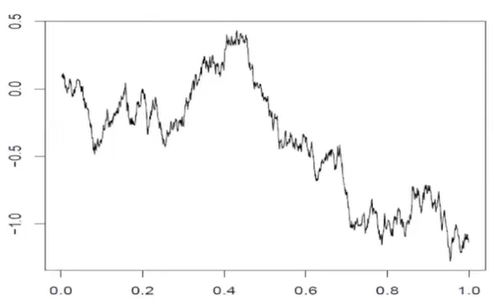
\includegraphics[width=.7\textwidth]{BrownianMotionExample.PNG}
    \caption{An example of Brownian Motion.}
    \label{fig_brownian_motion_example}
  \end{figure}

  \begin{remark}{Relevance Brownian Motion}
    \textit{Brownian Motion} can be used to construct a good model for prices (See \texttt{Figure \ref{fig_brownian_motion_example}}). Brownian motion is not smooth but generally shows a particular trend/drift.
  \end{remark}

  \begin{definition}{$S_t^{(n)}$}\label{def_S_t_n}
    Let $\{S_j\}_{j\in\nats}$ be a \textit{Random Walk} defined by $S_0=0$ and $S_n=S_{n-1}+X_n$ where $X_1,X_2,\dots$ are IID random variables with mean 0 and variance 1.
    \par Define a process $\{S_t^{(n)}\}_{t\in[0,1]}$ on $[0,1]$ by setting $S_t^{(n)}=S_j/\sqrt{n}$ for every $t=j/n$ and linearly interpolate in between.
  \end{definition}

  \begin{proposition}{Properties of $S_t^{(n)}$}
    Here are some properties of $\{S_t^{(n)}\}_{t\in[0,1]}$
    \begin{enumerate}
      \item $S_0^{(n)}=S_0/\sqrt{n}=0$.
      \item Taking $t=j/n$ and $u=k/n$ gives
      \[ S_{t+u}^{(n)}-S_t^{(n)}=(S_{j+k}-S_j)/\sqrt{n}=(X_{j+1}+\dots+X_{j+k})/\sqrt{n} \]
      As the $X$s are independent, this shows that the change in value of a given period is independent of both the start and end points.
      \item Taking $t=j/n$ and $u=k/n$, for large $n$. Consider this expression for the change in value over a time period
      \[ S_{t+u}^{(n)}-S_t^{(n)}=\frac{X_{j+1}+\dots+X_{j+k}}{\sqrt{n}}=\frac{\sqrt{k}}{\sqrt{n}}\left(\sum_{i=j+1}^{j+k}\frac{X_i}{\sqrt{k}}\right) \]
      By the \textit{Central Limit Theorem} this tends to $\text{Normal}\left(0,k/n\right)=\text{Normal}\left(0,u\right)$.
      \item $S_t^{(n)}(\omega)$ is continuous as a function of $t$, for all $n$ and all $\omega\in\Omega$.
      \item As $n\to\infty$, $S_t^{(n)}$ tends to a process $W_t$ known as \textit{Brownian Motion}.
    \end{enumerate}
  \end{proposition}

  \begin{theorem}{Theorem of Donsher\footnote{AKA \textit{Functional Central Limit Theorem}}}
    \textit{NON-EXAMINABLE}
    \par For every bounded and continuous function $h:C(0,1)\to\reals$
    \[ \expect\left[h(\{S_t^{(n)}\}_{t\in[0,1]})\right]\longrightarrow\expect\left[h(\{W_t\}_{t\in[0,1]})\right] \]
  \end{theorem}

  \begin{definition}{Brownian Motion\footnote{AKA \textit{Wiener Process}}}\label{def_brownian_motion}
    Let $\mathcal{F}_t$ be a \textit{Filtration}.
    \par An \textit{Adapted Stochastic Process} $W:=\{W_t\}_{t\geq0}$ is a standard one-dimensional \textit{Brownian Motion} if
    \begin{enumerate}
      \item $W_0=0$ (Almost surely)
      \item $W$ has independent increments. (i.e. $W_{t+u}-W_t$ is independent of $\mathcal{F}_t$ for all $u,t\geq0$.)
      \item $W$ has stationary Gaussian increments. (i.e. $W_{t+u}-W_t$ is normally distributed with mean 0 and variance $u$.)
      \item $W$ has continuous paths. ($W_t(\omega)$ is a continuous function of $t$ for all $\omega\in\Omega$.)
    \end{enumerate}
  \end{definition}

  \begin{theorem}{Wiener}
    The existence of \textit{Brownian Motion} was proved by \textit{Wiener} in 1923. That's the theorem.
  \end{theorem}

  \begin{proposition}{Properties of Standard Brownian Motion}\label{pro_properties_of_standard_brownian_motion}
    Let $W_t$ be \textit{Standard Brownian Motion}. Then
    \begin{enumerate}
      \item $\expect[X_t]=0,\ \var(W_t)=t\ \forall\ t$.
      \item $\forall\ s,t\ \cov(W_s,W_t)=\min\{s,t\}$.
      \item $-W_t$ is \textit{Standard Brownian Motion}.
      \item For fixed $t$, $X_s:=W_{s+t}-W_t$ is \textit{Standard Brownian Motion}. (i.e. You can move the start point).
      \item For any $\alpha$, $y_s:=W_{\alpha s}/\sqrt\alpha$ is \textit{Standard Brownian Motion}. (i.e. If you zoom in to see a day, rather than a week, the same properties hold).
    \end{enumerate}
  \end{proposition}

  \begin{proof}{\texttt{Theorem \ref{sec_stochastic_processes_in_continuous_time}.\ref{pro_properties_of_standard_brownian_motion}} i)-v)}
    \begin{enumerate}
      \item Follows from properties i) \& iii) of \texttt{Definition \ref{sec_stochastic_processes_in_continuous_time}.\ref{def_brownian_motion}}.
      \item By the previous result we can conclude that
      \[\begin{array}{rcl}
        \cov(W_s,W_t)&=&\expect[W_s\cdot W_t]\\
        &=&\expect[W_s\cdot(W_t-W_s)]+\expect[W_s^2]\\
        &=&\expect[W_s\cdot(W_t-W_s)]+\underbrace{\var(W_s)}_{=s}\\
        &=&\underbrace{\expect[W_s]}_{=0}\expect[W_t-W_s]+s\\
        &=&s
      \end{array}\]
      \item $\expect[-W_t]=-\expect[W_t]=0$ and increments occur in the $t$-direction, not the $X$-direction, so the distribution of $W_{t+u}-W_t$ is unaffected.
      \item In the case $t=0$ we find that $X_0=W_t-W_t=0$. The other properties in \texttt{Defintion \ref{sec_stochastic_processes_in_continuous_time}.\ref{def_brownian_motion}} are shift-invariant and therefore follow as well.
      \item The main part to check here is propert iii) of \texttt{Defintion \ref{sec_stochastic_processes_in_continuous_time}.\ref{def_brownian_motion}}. Indeed
      \[\begin{array}{rcl}
        Y_{t+s}-Y_t&=&\underbrace{(W_{\alpha(t+s)}-W_{\alpha t})}_{\sim\text{Nor}(0,\alpha s)}/\sqrt{\alpha}\\
        &\sim&\text{Normal}(0,s)
      \end{array}\]
    \end{enumerate}
    \proved
  \end{proof}

  \begin{proposition}{More properties of Brownian Motion}\label{pro_more_properties_of_brownian_motion}
    Let $\{W_t\}_{t\geq0}$ be \textit{Standard Brownian Motion} wrt \textit{Filtration} $\{\mathcal{F}_t\}$. Then
    \begin{enumerate}
      \item $\{W_t\}_{t\geq0}$ is a \textit{Martingale}.
      \item $\{W_t^2-t\}_{t\geq0}$ is a \textit{Martingale}.
      \item $\forall\ \lambda\in\reals$, the process $\{Z_t\}_{t\geq0}$ defined as
      \[ Z_t=\exp\left\{\lambda W_t-\frac12\lambda^2t\right\} \]
      is a \textit{Martingale}.
      \par More generally, the \textit{Geometric Brownian Motion} with volatility $\sigma>0$ and drift $a\in\reals$ can be defined as
      \[ \tilde{Z}_t=\exp\left\{\sigma W_t+at\right\} \]
      and is a \textit{Martingale} \underline{iff} $a=-\sigma^2/2$.
    \end{enumerate}
  \end{proposition}

  \begin{proof}{\texttt{Proposition \ref{sec_stochastic_processes_in_continuous_time}.\ref{pro_more_properties_of_brownian_motion}}}
    \begin{enumerate}
      \item We can write $W_t=(W_t-W_s)+W_s$. As $(W_t-W_s)$ is independent of filtration $\mathcal{F}_s$ and has zero mean, we can conclude that
      \[ \expect[W_t|\mathcal{F}_s]=\expect[W_t-W_s|\mathcal{F}_s]+\expect[W_s|\mathcal{F}_s]=\underbrace{\expect[W_t-W_s]}_{=0}+W_s=W_s \]
      \item Similarly, we can write
      \[ W_t^2=(W_t-W_s)^2+2W_s(W_t-W_s)+W_s^2 \]
      Then
      \[\begin{array}{rcl}
        \expect[W_t^2-t|\mathcal{F}_s]&=&\left\{\expect[(W_t-W_s)^2|\mathcal{F}_s]+2W_s\expect[W_t-W_s|\mathcal{F}_s]+W_s^2\right\}-t\\
        &=&\var(W_t-W_s)+0+W_s^2-t\\
        &=&t-s+W_s^2-t\\
        &=&W_s^2-s
      \end{array}\]
      \item We find that
      \[\begin{array}{rcl}
        \expect[\tilde{Z}_t|\mathcal{F}_s]&=&\expect[\exp\{\sigma W_t+at\}|\mathcal{F}_s]\\
        &=&\exp\{at\}\expect[\exp\{\sigma(W_t-W_s+W_s)\}|\mathcal{F}_s]\\
        &=&\exp\{\sigma W_s+at\}\cdot\expect[\exp\{\sigma\overbrace{(W_t-W_s)}^{:=N}\}|\mathcal{F}_s]\\
        &=&\exp\{\sigma W_s+at\}\expect[\exp\{\sigma N\}|\mathcal{F}_s]\\
        &=&\exp\{\sigma W_s+at\}\expect[\exp\{\sigma N\}]
      \end{array}\]
      where $N\sim\text{Normal}(0,t-s)$. The MGF of $N$ is $\expect[e^{\sigma N}]=e^{(t-s)\sigma^2/2}$, therefore
      \[\begin{array}{rcl}
        \expect[\tilde{Z}_t|\mathcal{F}_s]&=&\exp\{\sigma W_s+at\}\expect[\exp\{\sigma N\}]\\
        &=&\tilde{Z}_se^{a(t-s)}e^{(t-s)\sigma^2/2}\\
        &=&\tilde{Z}_s\exp\left\{(t-s)\left(a+\frac{\sigma^2}2\right)\right\}
      \end{array}\]
      We conclude that $\tilde{Z}_t$ is a \textit{Martingale} \underline{iff} $a=-\sigma^2$\footnote{As we require $\expect[\tilde{Z}_t|\mathcal{F}_s]=\tilde{Z}_s$ which only occurs \underline{iff} $a+\frac{\sigma^2}2=0$.}.
    \end{enumerate}
    \proved
  \end{proof}

\subsection{Stochastic Integration}

  \begin{remark}{Motivation}
    Ideally we could evaluate our trading strategy $H(t)$ by integrating it over all possible paths of the stock price (e.g. Brownian Motion $W(t)$)
    \[ \int_0^TH(t)dW(t) \]
    For a differentiable function $g(\cdot)$ it holds that
    \[ \int_0^TH(t)dg(t)=\int_0^TH(t)g'(t)dt \]
    However, the price process $W(t)$ is \underline{not} differentiable and thus we have to take another approach.
  \end{remark}

  \begin{figure}[H]
    \centering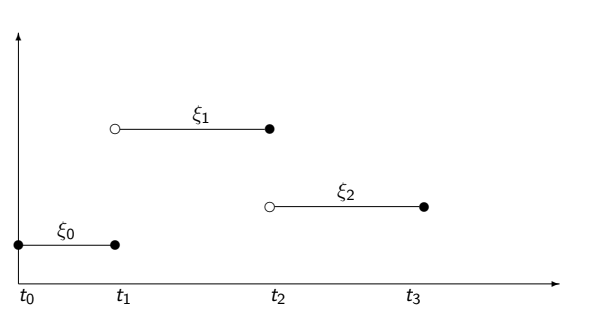
\includegraphics[width=.7\textwidth]{SimpleStochasticProcess.PNG}
    \caption{Example of Simple Stochastic Process}
    \label{fig_simple_stochastic_process}
  \end{figure}

  \begin{definition}{Simple Stochastic Process}
    A \textit{Stochastic Process} $X:=\{X_t\}_{t\in[0,T]}$ is said to be \textit{Simple} if there exists a partition
    \[ 0=t_0<t_1<\dots<t_n=T \] and a set of $\mathcal{F}_{t_k}$-measurable random variables $\{\xi_k\}_{k\in[0,n]}$, which all satisfy $\expect[|\xi_k|]<\infty$, st $X_t(\omega)$ can be written in the form
    \[ X_t(\omega)=\xi_0(\omega)\indexed\{t=0\}+\sum_{i=0}^{n-1}\xi_i(\omega)\indexed\{t\in[t_i,t_{i+1}]\} \]
    This produces a stepped function (See \texttt{Figure \ref{fig_simple_stochastic_process}}).
  \end{definition}

  \begin{definition}{Stochastic Integral}
    Let $X:=\{X_t\}_{0\in[0,T]}$ be a \textit{Simple Stochastic Process}.
    \par We define the \textit{Stochastic Integral} $I_t(\cdot)$ of $X$ as
    \[ I_t(X):=\int_0^tXdW=\sum_{i=0}^{n-1}\xi_i\cdot\left(W_{\min(t,t_{i+1})}-W_{\min(t,t_i)}\right) \]
    where $W_t$ is \textit{Brownian Motion}.
  \end{definition}

  \begin{remark}{Stochastic Integral is a Stochastic Process}
    For each $t$, $I_t(X)$ is a random variable.
    \par Thus, $\{I_t(X)\}_t$ is a \textit{Stochastic Process}.
  \end{remark}

  \begin{remark}{Stochastic Integral Expanding}
    If $t\in[t_k,t_{k+1}]$ for some $k\in[0,n-1]$ then
    \[ I_t(X)=\left\{\sum_{i=0}^{k-1}\xi_i\cdot(W_{t_{i+1}}-W_{t_i})\right\}+\xi_k\cdot(W_t-W_{t_k}) \]
  \end{remark}

  \begin{example}{Stochastic Integrals}
    \begin{enumerate}
      \item Consider the simple stochastic process $\{X_t\}_{t\in[0,T]}$ where $X_t=c\ \forall\ t$. This is arguably the simplest random process possible and means $n=1$ in the partition. Then
      \[ I_t(X)=cW_t \]
      \item Suppose each $X_t=X$ which is random, but fixed for all $t$. This means $n=1$ in the partition and
      \[ I_t(X)=XW_t \]
      \item Suppose $X_t=c$ for $t\leq1/2$ and $X_t=d$ for $t>1/2$. Then
      \[ I_t(X)=\begin{cases}cW_t&\text{if }t<1/2\\cW_{1/2}+d(W_t-W_{1/2})&\text{if }t\geq1/2\end{cases} \]
    \end{enumerate}
  \end{example}

  \begin{theorem}{Properties of Simple Stochastic Processes}\label{the_properties_of_simple_stochastic_processes}
    Let $X:=\{X_t\}_{t\in[0,T]}$ be a \textit{Simple Stochastic Process}. Then
    \begin{enumerate}
      \item The expectation of its \textit{Stochastic Process} is zero
      \[ \expect[I_t(X)]=0 \]
      \item The \textit{Stochastic Process} satisfies It\^o's isometry
      \[ \expect\left[(I_t(X))^2\right]=\int_0^t\expect[X_s^2ds] \]
      \item $I_t(X)$ is a continuous \textit{Martingale} wrt the \textit{Natural Brownian Motion Filtration} $\mathcal{F}_t$ for all $0\leq s\leq t\leq T$.
      \[ \expect\left[I_t(X)|\mathcal{F}_s\right]=I_s(X) \]
      \item \textit{Linearity} - Let $Y$ be another \textit{Simple Stochastic Process} and $a,b$ be arbitrary real numbers. Then
      \[ I_t(aX+bY)=aI_t(X)+bI_t(Y) \]
      \item The stochastic process $I_t(X)$ has continuous sample paths.
    \end{enumerate}
  \end{theorem}

  \begin{proof}{\texttt{Theorem \ref{sec_stochastic_processes_in_continuous_time}.\ref{the_properties_of_simple_stochastic_processes}}}
    \everymath={\displaystyle}
    \begin{enumerate}
      \item Note that since $\xi_i$ is $\mathcal{F}_{t_i}$ measurable, then $\xi_i$ \& $(W_{t_{i+1}}-W_{t_i})$ are independent for all $i$. Also $\expect[W_{t_{i+1}}-W_{t_i}]=0$, thus
      \[ \expect[\xi_i(W_{t_{i+1}}-W_{t_i})]=\expect[\xi_i]\expect[W_{t_{i+1}}-W_{t_i}]=0 \]
      Meaning
      \[ \expect[I_t(X)]=0 \]

      \item Consider a partition of $[0,t]$ st $0=t_0<\dots<t_k=t$. Then
      \[ \expect[(I_t(X))^2]=\sum_{i=0}^{k-1}\sum_{j=0}^{k-1}\expect\left[\xi_i(W_{t_{i+1}}-W_{t_i})\xi_j(W_{t_{j+1}}-W_{t_j})\right] \]
      If $i>j$ then $(W_{t_{i+1}}-W_{t_i})$ is independent of all the other factors and has expectation 0
      \[\begin{array}{rl}
        \expect\left[\xi_i(W_{t_{i+1}}-W_{t_i})\xi_j(W_{t_{j+1}}-W_{t_j})\right]\\
        =&\underbrace{\expect[\underbrace{W_{t_{i+1}}-W_{t_i}}_{\sim N(0,t_{i+1}-t_i)}]}_{=0}\expect[\xi_i\xi_j(W_{t_{j+1}}-W_{t_j})]
      \end{array}\]
      So all terms with $i>j$ and, similarly $i<j$, disappear and we conclude that
      \[\begin{array}{rcl}
        \expect[I_t(X)^2]&=&\sum_{i=0}^{k-1}\expect[\xi_i(W_{t_{i+1}}-W_{t_i})\xi_i(W_{t_{i+1}}-W_{t_i})]\\
        &=&\sum_{i=0}^{k-1}\expect[\xi_i^2]\expect[(W_{t_{i+1}}-W_{t_i})^2]\\
        &=&\sum_{i=0}^{k-1}\expect[\xi_i^2](t_{i+1}-t_i)
      \end{array}\]
      The last step comes from considering the variance of $(W_{t_{i+1}}-W_{t_i})$.
      \par The RHS is the usual Riemann Integral $\int_0^Tf(s)ds$ of the step function $f(x)=\expect[X_s^2]$ which coincides with $\expect[\xi^2]$ for $s\in[t_i,t_{i+1}]$.

      \item Adaptedness of $I(X)$ follows since at time $t$ all $\xi_i$ and $(W_{t_{i+1}}-W_{t_i})$ contributing to $I_t(X)$ are functions of \textit{Brownian Motion} up to time $t$.
      \par The condition $\expect\left[\left|I_t(X)\right|\right]$ follows from the isometry property ii).
      \par It remains to show that $\expect\left[I_t(X)|\mathcal{F}_s\right]$ for all $s<t$.
      \par First, assume that $s<t$ and $s,t\in[t_k,t_{k+1}]$. Notice that
      \[\begin{array}{rcl}
        I_t(X)&=&I_{t_k}(X)+\xi_k(W_t-W_{t_k})\\
        I_s(X)&=&I_{t_k}(X)+\xi_k(W_s-W_{t_k})
      \end{array}\]
      Hence $I_t(X)=I_s(X)+\xi_k(W_t-W_s)$ where $I_s(X)$ and $\xi_k$ are known at time $s$, and $(W_t-W_s)$ is independent of $\mathcal{F}_s$ and has mean zero. Hence
      \[ \expect\left[I_t(X)|\mathcal{F}_s\right]=I_s(X)+\xi_k\underbrace{\expect\left[W_t-W_s\right]}_{=0}=I_s(X) \]
      The case where $s<t_k<t$ can be handled analogously.

      \item Assume that the simple process $X$ is defined using the partition
      \[ 0=t_0<t_1<\dots<t_n=T \]
      and $Y$ uses the partition
      \[ 0=s_0<s_1<\dots<s_m=T \]
      Note that these partitions can be different lengths and take different values.
      \par Consider the joint-partition
      \[ 0=u_0<u_1<\dots<u_l=T \]
      which combines all the points from the other partitions, ensuring the correct ordering of values. The values of $I_t(X)$ and $I_t(Y)$ wrt the finer partition $\{u_0,\dots,u_l\}$ remain the same.
      \par Linearity follows from the linearity of the underlying sums.

      \item This follows from the definition of $I_t(X)$ since
      \[ I_t(X)=I_{t_{k-1}}(X)+\xi_k(W_t-W_{t_{k-1}})\ \forall\ t\in[t_{k-1},t_k] \]
      The only unfixed term in this expression is the \textit{Brownian Motion} $W_t$. We know that \textit{Brownian Motion} has continuous sample paths, thus $I_t(X)$ has continuous sample paths.
    \end{enumerate}
  \end{proof}

  \begin{theorem}{}\label{the_4_13}
    Let $X:=\{X_t\}_{t\in[0,T]}$ be a \textit{Stochastic Process} which is adapted to \textit{Brownian Motion}\footnote{i.e. $X_t$ is a function of $W_s$ for $s\leq$ which satisfies that $\int_0^T\expect[X_t^2]<\infty$}.
    \par Then one can find a sequence $X^{(n)}$ of simple processes st
    \[ \int_0^T\expect\left[(X_s-X_s^{(n)})^2\right]ds\overset{n\to\infty}{\longrightarrow}0 \]
    Moreover, there is some process $I(X)$ on $[0,T]$ st
    \[ \expect\left[\sup_{t\in[0,T]}\left(I_t(X)-I_t(X^{(n)})\right)^2\right]\overset{n\to\infty}{\longrightarrow}0 \]
  \end{theorem}

  \begin{definition}{It\^o Stochastic Integral}
    The mean square limit $I(X)$ in \texttt{Theorem \ref{sec_stochastic_processes_in_continuous_time}.\ref{the_4_13}} is called the \textit{It\^o Stochastic Integral} of $X$.
    \par It is denoted by
    \[ I_t(X):=\int_0^tX_sdW_s\quad t\in[0,T] \]
  \end{definition}

  \begin{remark}{Rule of Thumb for It\^o Stochastic Integral}
    The \textit{It\^o Stochastic Integral} $\{I_t(X)\}_{t\in[0,T]}$ constitute a \textit{Stochastic Process}. For a given partition $0=t_0<t_1<\dots<t_n=T$ and $t\in[t_k,t_{k+1}]$ the random variable $I_t(X)$ is approximately
    \[ I_t(X)\simeq\sum_{i=0}^{k-1}\left\{X_{t_i}(W_{t_{i-1}}-W_{t_i})\right\}+X_{t_k}(W_t-W_{t_k}) \]
    This approximation is closer to the value of $I_t(X)$ the denser the partition is in $[0,T]$.
  \end{remark}

    \begin{theorem}{Properties of It\^o Stochastic Integral\footnote{The proof for these properties is not covered in this course.}}\label{the_properties_of_ito_stochastic_integral}
      Let $X:=\{X_t\}_{t\in[0,T]}$ be a stochsatic process which satisfies the requirements of \texttt{Theorem \ref{sec_stochastic_processes_in_continuous_time}.\ref{the_4_13}}. Then
      \begin{enumerate}
        \item The stochastic integral $I_t(X)$ has expectation zero.
        \item The stochastic integral $I_t(X)$ satisfies the It\^o Isometry Property (\texttt{Theorem \ref{sec_stochastic_processes_in_continuous_time}.\ref{the_properties_of_simple_stochastic_processes}}).
        \item The stochastic integral $I_t(X)$ is a \textit{Martingale} wrt the \textit{Natural Brownian Filtration}.
        \item The stochastic integral $I_t(X)$ is \textit{Linear}.
        \item The stochastic integral $I_t(X)$ has continuous sample paths.
      \end{enumerate}
    \end{theorem}

    \begin{example}{Stochastic Integral of Brownian Motion}\label{ex_stochatic_integral_of_brownian_motion}
      \everymath={\displaystyle}
      We calculate the stochastic integral of Brownian motion
      \[ I_t(W)=\int_0^tW_sdW_s \]
      We start by approximating the integrand $W_s$ by a sequence of simple functions
      \[
        X_u^{(n)}=\begin{cases}
          W_0=0&\text{if }u\in[0,t_1]\\
          W_{t_1}&\text{if }u\in[t_1,t_2]\\
          \vdots\\
          W_{t_{n-1}}&\text{if }u\in[t_{n-1},t]
        \end{cases}\text{ where }t_k=\frac{tk}n\text{ for }k=0,1,\dots,n\footnotemark
       \]
       \footnotetext{The partition is equally spaced.}
       Then
       \[\begin{array}{rcl}
         I_t(X^{(n)})&=&\sum_{k=0}^{n-1}X_{t_k}^{(n)}(W_{t_{k+1}}-W_{t_k})\\
         &=&\sum_{k=0}^{n-1}W_{t_k}(W_{t_{k+1}}-W_{t_k})\\
         &=&\sum_{k=0}^{n-1}\left\{W_{t_{k+1}}W_{t_k}-W_{t_k}^2\right\}\\
         &=&\left\{\sum_{k=0}^{n-1}W_{t_{k+1}}W_{t_k}\right\}-\frac12\left\{\sum_{k=0}^{n-1}(W_{t_{k+1}}^2+W_{t_k}^2)\right\}+\frac12W_{t_n}^2\\
         &=&\frac12W_t^2-\frac12\sum_{k=0}^{n-1}(W_{t_{k+1}}-W_{t_k})^2\\
       \end{array}\]
       Since the increments $(W_{t_{k+1}}-W_{t_k})$ are independent and normally distributed with mean 0 and variance $t_{k+1}-t_k=t/n$, the sum of the RHS converges to t as $n\to\infty$. Thus we obtain
       \[ I_t(W)=\int_0^tW_sdW_s=\frac12W_t^2-\frac12 \]
    \end{example}

    \begin{remark}{\texttt{Example \ref{sec_stochastic_processes_in_continuous_time}.\ref{ex_stochatic_integral_of_brownian_motion}}}
      The argument used in \texttt{Example \ref{sec_stochastic_processes_in_continuous_time}.\ref{ex_stochatic_integral_of_brownian_motion}} leads to a general principle.
      \par If we write $\Delta W_{t_k}:=W_{t_{k+1}}-W_{t_k}$ and $\Delta t_k:=t_{k+1}-t_k$ then we can derive the following mean square limit properties
      \[\begin{array}{rcl}
        \sum_{k=0}^{n-1}(\Delta W_{t_k})^2&\overset{n\to\infty}{\longrightarrow}&t\sum_{k=0}^{n-1}\Delta W_t\Delta t_k\overset{n\to\infty}{\longrightarrow}0\\
        \sum_{k=0}^{n-1}(\Delta t_k)^2&\overset{n\to\infty}{\longrightarrow}&0
      \end{array}\]
      These are often written as the formal multiplication rules
      \[\begin{array}{rcl}
        dW\cdot dW&=&dt\\
        dt\cdot dW&=&0\\
        dt\cdot dt&=&0
      \end{array}\]
    \end{remark}

\subsection{It\^o's Lemma}

  \begin{theorem}{It\^o's Lemma - Special Case}\label{the_ito_v1}
    \textit{This is a special case of It\^o's Lemma.}
    \par Let $f(x)$ be a twice continuously differentiable function. Then for any $t>0$
    \[ f(W_t)-f(W_0)=\underbrace{\int_0^tf'(W_u)dW_u}_\text{Standard Integral}+\underbrace{\frac12\int_0^tf''(W_u)du}_\text{Stochastic Integral} \]
    or in differential form
    \[ df(W_t)=f'(W_t)dW_t+\underbrace{\frac12f''(W_t)dt}_\text{It\^o's Correction Term} \]
  \end{theorem}

  \begin{proof}{\texttt{Theorem \ref{sec_stochastic_processes_in_continuous_time}.\ref{the_ito_v1}}}
    Consider a partition $\{t_0,\dots,t_n\}$ of $[0,t]$ with $0=t_0<\dots<t_n=t$.
    \par By Taylor's formula we obtain
    \[\begin{array}{rcl}
      f(W_t)-f(W_0)&=&\sum_{i=0}^{n-1}f(W_{t_{i+1}})-f(W_{t_i})\\
      &=&\sum_{i=0}^{n-1}f'(W_{t_i})(W_{t_{i+1}}-w_{t_i})\\
      &+&\frac12\sum_{i=0}^{n-1}f''(W_{t_i}+\theta_i(W_{t_{i+1}}-W_{t_i}))(W_{t_{i+1}}-w_{t_i})^2\text{ with }\theta_i\in(0,1)
    \end{array}\]
    The first sum is an approximating sequence of a stochastic integral. Indeed, we find
    \[ \sum_{i=0}^{n-1}f'(W_{t_i})(W_{t_{i+1}}-W_{t_i})\overset{n\to\infty}\longrightarrow\int_0^tf'(W_u)dW_u \]
    We also know that
    \[ \lim_{n\to\infty}\sum_{i=0}^{n-1}(W_{t_{i+1}}-W_{t_i})^2=t \]
    and with a little more effort we can prove that\footnote{Proof is beyond scope of course. Won't be asked to reproduce this step.}
    \[ \lim_{n\to\infty}\sum_{i=0}^{n-1}f''(W_{t_i}+\theta_i(W_{t_{i+1}}-W_{t_i}))(W_{t_{i+1}}-W_{t_i})^2=\int_0^tf''(W_u)du \]
  \end{proof}

  \begin{example}{\texttt{Theorem \ref{sec_stochastic_processes_in_continuous_time}.\ref{the_ito_v1}}}
    Consider the function $f(x)=x^2$. Then
    \[ f'(x)=2x\quad f''(x)=2 \]
    By \texttt{Theorem \ref{sec_stochastic_processes_in_continuous_time}.\ref{the_ito_v1}} we have
    \[ W_t^2=f(W_t)-f(W_0)=\int_0^t2WudW_u+\frac12\int_0^t 2du=\int_0^t2W_udW_u+t \]
    Hence
    \[ \frac12(W_t^2-t)=\int_0^tW_udW_u \]
    as in \texttt{Example \ref{sec_stochastic_processes_in_continuous_time}.\ref{ex_stochatic_integral_of_brownian_motion}}
  \end{example}

  \begin{theorem}{It\^o's Lemma - More General Case}\label{the_ito_v2}
    \textit{This is a more general case of It\^o's Lemma than \texttt{Theorem \ref{sec_stochastic_processes_in_continuous_time}.\ref{the_ito_v1}}, but not as general as \texttt{Theorem \ref{sec_stochastic_processes_in_continuous_time}.\ref{the_ito_v3}}.}
    \par Let $f(t,x)$ be a function which is continuously differentiable once in its first argument (the time parameter $t$) and twice in its second argument $x$. Then

    \[ f(t,W_t)-f(0,W_0)=\int_0^tf_t(u,W_u)+\frac12 f_{xx}(u,W_u)du +\int_0^tf_x(u,W_i)dW_u\]
    where $f_t:=\frac{\partial f}{\partial t},\ f_{xx}:=\frac{\partial^2 f}{\partial x^2}$ and $f_x:=\frac{\partial f}{\partial x}$.
    \par Or, in differentiable form
    \[ df(t,W_t)=(f_t(t,W_t)+\frac12f_{xx}(t,W_t))dt+f_x(t,W_t)dW_t \]
  \end{theorem}

  \begin{proof}{\texttt{Theorem \ref{sec_stochastic_processes_in_continuous_time}.\ref{the_ito_v2}}}
    By the Taylor expansion of a smooth function of several variables we get for $t$ close to $t_0$ that
    \[\begin{array}{rcl}
      f(t,W_t)&=&f(t_0,W_{t_0})+(t-t_0)f_t(t_0,W_{t_0})+(W_t-W_{t_0})f_x(t_0,W_{t_0})\\
      &+&\frac12(t-t_0)^2f_{tt}(t_0,W_{t_0})+\frac12(W_t-W_{t_0})^2f_{xx}(t_0,W_{t_0})\\
      &+&(t-T_0)(W_t-W_{t_0})f_{tx}(t_0,W_{t_0})+\text{Higher order terms}
    \end{array}\]
    This can be written symbolically as
    \[ df=f_tdt+fxdW+\frac12f_{tt}(dt)^2+f_{tx}dtdW+\frac12f_{xx}(dW)^2+\dots \]
    Note that $(dt)^2=0$. Now using the formal multiplication rules
    \[ dt\cdot dt=0\quad dt\cdot dW=0\quad dW\cdot dW=dt \]
    We get
    \[ df=f_td_t+f_xdW+\frac12f_{xx}dt=(f_t+\frac12f_{xx})df+f_xdW \]
  \end{proof}

  \begin{example}{It\^o's Exponential}
    Consider the function
    \[ f(t,x)=\exp\left\{x-\frac{t}2\right\} \]
    Then
    \[ f_t=-\frac{f(t,x)}2\quad f_x(t,x)=f(t,x)\quad f_{xx}(t,x)=f(t,x) \]
    Thus, by \texttt{Theorem \ref{sec_stochastic_processes_in_continuous_time}.\ref{the_ito_v2}} , since $f(0,W_0)=1$.
    \[\begin{array}{rcl}
      f(t,W_t)-1&=&\int_0^t-\frac12f(u,W_u)+\frac12 f(u,W_u)du+\int_0^tf(u,W_u)dW_u\\
      &=&\int_0^tf(u,W_u)dW_u
    \end{array}\]
    Note that this is a stochastic integral.
    \par Hence $f$ satisfies the differential equation $df=fdW$ in the It\^0 sense and is therefore called the It\^o exponential.
  \end{example}

  \begin{example}{Geometric Brownian Motion}
    Consider the function
    \[ f(t,x)=\exp\left\{\sigma x+(\mu-\frac{\sigma^2}2)t\right\} \]
    Then
    \[ f_t(t,x)=\left(\mu-\frac{\sigma^2}2\right)f(t,x)\quad f_x(t,x)=\sigma f(t,x)\quad f_{xx}(t,x)=\sigma^2f(t,x) \]
    Thus $f_t+\frac{f_{xx}}2=\mu f(t,x)$. So by \texttt{Theorem 4.20}
    \[ f(t,W_t)-f(0,W_0)=\int_0^t\mu f(u,W_u)du+\int_0^t\sigma f(u,W_u)dW_u \]
    The process $X_t=f(t,W_t)$ satisfies the linear stochastic differential equation
    \[ X_t-X_0=\mu\int_0^tX_sds+\sigma\int_0^tX_sdW_s \]
    In differential notation this is
    \[ dX=\mu Xds+\sigma XdW=X(\mu ds+\sigma dW) \]
    This is useful for geometric Brownian motion when $\mu$ is the drift term and $\sigma$ is the volatility.
  \end{example}

  \begin{definition}{It\^o Process}
    Let $X=\{X_t\}_{t\in[0,T]}$ be a stochastic process such that
    \[ X_t=X_0+\int_0^tb_udu+\int_0^t\sigma_udW_u \]
    where both $b,\sigma$ are functions which are adapted to Brownian motion. This $X$ is called an \textit{It\^o Process}.
    \par We also say that the process $X$ has a stochastic differential
    \[ dX_t=b_td_t+\sigma_tdW_t \]
  \end{definition}

  \begin{theorem}{It\^o's Lemma - Most General}\label{the_ito_v3}
    Let $X$ be an \textit{It\^o Process} and $f(t,x)$ be a function  whose second order partial derivatives are continuous. Then for any $t>0$
    \[ f(t,X_t)-f(0,X_0)=\int_0^tf_t(u,X_u)+b_uf_x(u,X_u)+\frac12\sigma^2_uf_{xx}(u,X_u)du+\int_0^t\sigma_uf_x(u,X_u)dW_u \]
    Or in differential form
    \[ df=\left(f_t+b_tf_X+\frac12\sigma_t^2f_{xx}\right)dt+\sigma_tf_xdW_t \]
  \end{theorem}

  \begin{proof}{\texttt{Theorem \ref{sec_stochastic_processes_in_continuous_time}.\ref{the_ito_v3}}}
    We proceed as in the preceding version of It\^o's formula and consider a Taylor expansion of $f(t,X_t)$ which is in differential notation
    \[ df=f_tdt+f_xdX+\frac12f_{tt}(dt)^2+f_{tx}dtdx+\frac12f_{xx}(dX)^2+\text{High order terms} \]
    Now we substitute $dX=bdt+\sigma dW$ and obtain
    \[\begin{array}{rcl}
      df&=&f_tdt+f_x(bd_t+\sigma dW)+\frac12f_{tt}(dt)^2+f_{tx}dt(bdt+\sigma dW)+\frac12f_{xx}(bd_t+\sigma dW)+\text{High order terms}
    \end{array}\]
    Again, neglecting all $(ft)^2)$ and $dtdW$ terms as well as the high order terms we obtain
    \[\begin{array}{rcl}
      df&=&f_td_t+f_x(bd_t+\sigma dW)+\frac12f_{xx}(\sigma dW)^2\\
      &=&(f_t+f_xb+\frac12\sigma^2f_{xx})dt+f_x\sigma dW
    \end{array}\]
  \end{proof}

  \begin{theorem}{Product Rule for Stochastic Calculus}\label{the_product_rule_stochastic_calculus}
    \textit{We can derive the produce rule for stochastic calculus from \texttt{Theorem \ref{sec_stochastic_processes_in_continuous_time}.\ref{the_ito_v3}}.}
    \par Suppose two process $X_t,Y_t$ are adapated to the same Brownian motion
    \[\begin{array}{rcl}
      dX_t&=&\sigma_tdW_t+\mu_tdt\\
      dY_t&=&\rho_tdW_t+\nu_tdt
    \end{array}\]
    Then
    \[ d(X_tY_t)=X_tdY_t+Y_tdX_t+\sigma_t\rho_tdt \]
  \end{theorem}

  \begin{proof}{\texttt{Theorem \ref{sec_stochastic_processes_in_continuous_time}.\ref{the_product_rule_stochastic_calculus}}}
    Since $d(X_t+Y_t)=(\sigma_t+\rho_t)dW_t+(\mu_t+\sigma_t)dt$, using \texttt{Theorem \ref{sec_stochastic_processes_in_continuous_time}.\ref{the_ito_v3}} applied to $f(t,x)=x^2$ we obtain that
    \[\begin{array}{rcl}
      d(X_t^2)&=&(2\mu_tX_t+\sigma_t^2)dt+2\sigma_tX_tdW_t\\
      d(Y_t^2)&=&(2u\nu_tY_t+\rho_t^2)dt+2\rho_tY_tdW_t\\
      d((X_t+Y_t)^2)&=&(2(\mu_t+\nu_t)(X_t+Y_t)+(\sigma_t+\rho_t)^2)dt\\
      &+&2(\sigma_t+\rho_t)(X_t+Y_t)dW_t
    \end{array}\]
    Subtracting, the result follows since
    \[\begin{array}{rcl}
      2d(X_tY_t)=d((X_t+Y_t)^2-X_t^2-Y_t^2)\\
      &=&2(\mu_tY_t+\nu_tX_t)dt+2\sigma_t\rho_tdt+2(\sigma_tY_t+\rho_tX_t)dW_t\\
      &=&2Y_tdX_t+2X_tdY_t+2\sigma_t\rho_tdt
    \end{array}\]
  \end{proof}

  \begin{example}{Geometric Brownian Motion}
    
  \end{example}

  \begin{example}{Ornstein-Uhlenbeck Process}

  \end{example}

\section{Financial Market Models in Continuous Time} \label{sec_financial_market_models_in_continuous_time}

\subsection{The Financial Market Model in Continuous Time}

\subsection{Trading Strategies}

\subsection{Arbitrage in the Continuous Time Model}

\subsection{The Black-Scholes Model}

\subsection{Equivalent Martingale Measures in the Black-Scholes Model}

\subsection{Pricing in the Black-Scholes Model}

\subsection{Replicating Strategies and the Black-Scholes-Merton Equation}

\reference
\section{Notation}

  \begin{notation}{General Mathematical Notation}
    \begin{tabular}{c|c}
      Notation&Description\\\hline
      $\{x\}_+$&Only the positive part of $x$ (i.e. $\max\{0,x\}$).
    \end{tabular}
  \end{notation}

\end{document}
